\documentclass[12pt]{book}
\usepackage{html,a4wide,epsfig}
\usepackage[british]{babel}
\newcommand{\hl}[1]{\htmladdnormallink{{\it #1}}{#1}}
\newcommand{\ix}[1]{#1\index{#1}}
\makeindex
\begin{document}
\pagenumbering{roman}
\pagestyle{empty}

\begin{center}
{\Huge\bf SWAN}
\end{center}
\vspace{2cm}
\begin{center}
{\Large\bf SCIENTIFIC\\ AND\\ TECHNICAL\\ DOCUMENTATION\\}
\end{center}
\vfill
\begin{center}
{\Large\bf SWAN Cycle III version 40.91}
\end{center}

\cleardoublepage

\noindent
{\Large\bf SWAN\\ SCIENTIFIC AND TECHNICAL\\ DOCUMENTATION\\}

\vfill

\begin{table}[htb]
\begin{tabular}{lcl}
by           &:& The SWAN team \\
             & & \\
mail address &:& Delft University of Technology \\
             & & Faculty of Civil Engineering and Geosciences \\
             & & Environmental Fluid Mechanics Section \\
             & & P.O. Box 5048 \\
             & & 2600 GA Delft \\
             & & The Netherlands \\
             & & \\
e-mail       &:& swan-info-citg@tudelft.nl \\
home page    &:& \hl{http://www.swan.tudelft.nl}
\end{tabular}
\end{table}

\vfill

\noindent
Copyright (c) 1993-2012 Delft University of Technology.
\\[2ex]
\noindent
Permission is granted to copy, distribute and/or modify this document
under the terms of the GNU Free Documentation License, Version 1.2
or any later version published by the Free Software Foundation;
with no Invariant Sections, no Front-Cover Texts, and no Back-Cover
Texts. A copy of the license is available at
\hl{http://www.gnu.org/licenses/fdl.html\#TOC1}.

\clearpage
\pagestyle{myheadings}
\newcommand{\chap}[1] % Re-define the chapter command
       {
        \chapter{#1}
        \markboth{\hfill Chapter \thechapter \hfill}{\hfill {#1} \hfill}
       }

\tableofcontents

\chap{Introduction} \label{ch:intro}
\pagenumbering{arabic}

The main goal of the SWAN model is to solve the spectral action balance equation without any {\em a priori}
restrictions on the spectrum for the evolution of wave growth. This equation represents the effects of
spatial propagation, refraction, shoaling, generation, dissipation and nonlinear wave-wave interactions.
The basic scientific philosophy of SWAN is identical to that of WAM cycle 3. SWAN is a third-generation wave
model and it uses the same formulations for the source terms.
\nocite{WAM88}
\\[2ex]
\noindent
Whereas the WAM model considers problems on oceanic scales, with SWAN wave propagation is calculated
from deep water to the surf zone. Since, WAM makes use of explicit propagation schemes in geographical and
spectral spaces, it requires very small grid sizes in shallow water and is thus unsuitable for applications
to coastal regions. For that reason, SWAN employs implicit schemes, which are more robust and economic
in shallow water than the explicit ones. Note that SWAN may be less efficient on oceanic scales than WAM.

\section{Historical background} \label{sec:hist}

Over the past two decades, a number of advanced spectral wind-wave models, known as
third-generation models, has been developed such as WAM (WAMDI Group, 1988), WAVEWATCH~III
(Tolman, 1991), TOMAWAC (Benoit~{\it et~al}., 1996) and SWAN (Booij~{\it et~al}., 1999).
These models solve the spectral action balance equation without any {\em a priori} restrictions
on the spectrum for the evolution of wave growth.
\\[2ex]
\noindent
Based on the wave action balance equation with sources and sinks, the shallow water
wave model SWAN (acronym for \underline{S}imulating \underline{WA}ves \underline{N}earshore)
is an extension of the deep water third-generation wave models.
It incorporates the state-of-the-art formulations for the deep water processes of
wave generation, dissipation and the quadruplet wave-wave interactions from the
WAM model (Komen~{\it et~al}., 1994). In shallow water, these processes have been
supplemented with the state-of-the-art formulations for dissipation due to bottom
friction, triad wave-wave interactions and depth-induced breaking. SWAN is fully
spectral (in all directions and frequencies) and computes the evolution of wind
waves in coastal regions with shallow water and ambient current.
\\[2ex]
\noindent
SWAN is developed at Delft University of Technology and is freely available from\\
\hl{http://www.swan.tudelft.nl}. It is used by many goverment
authorities, research institutes and consultants worldwide. The feedback has widely
indicated the reliability of SWAN in different experiment and field cases.
\\[2ex]
\noindent
Initially, the SWAN cycle 1 was formulated to be able to handle only stationary conditions
on a rectangular grid. Later on, SWAN cycle 2 model has been developed. This is considered
as the second step in the development of SWAN models. Cycle 2 of SWAN is stationary
and optionally nonstationary. It can compute the wave propagation not only on a regular
rectangular grid, but also on a curvi-linear grid. Previous official versions 30.62, 30.75,
40.01 and 32.10 belong to the cycle 2 of SWAN.
\\[2ex]
\noindent
This section is under preparation.

\section{Purpose and motivation} \label{sec:purp}

The purpose of this document is to provide relevant information on the mathematical models and numerical techniques for
the simulation of spectra of random short-crested, wind-generated waves in coastal regions. Furthermore, this document
explains the essential steps involved in the implementation of various numerical methods, and thus provides an adequate
reference with respect to the structure of the SWAN program.

\section{Readership} \label{sec:read}

This document is, in the first place, addressed to those, who wish to modify and to extend mathematical and numerical
models for shallow wind-wave problems. However, this material is also useful for those who are interested in the application
of the techniques discussed here. The text assumes the reader has basic knowledge of analysis, partial differential
equations and numerical mathematics and provides what is needed both in the main text and in the appendices.

\section{Scope of this document} \label{sec:scope}

SWAN is a third-generation wave model for
obtaining realistic estimates of wave parameters in coastal areas, lakes and estuaries from given wind, bottom and
current conditions. However, SWAN can be used on any scale relevant for wind-generated surface gravity waves. The model
is based on the wave action balance equation (or energy balance in the absence of currents) with sources and sinks.
Good introductory texts on the background of SWAN are Young (1999) and Booij~{\it et~al}. (1999).
\\[2ex]
\noindent
The following wave \underline{propagation} processes are represented in SWAN:
\begin{itemize}
 \item propagation through geographic space,
 \item refraction due to spatial variations in bottom and current,
 \item diffraction,
 \item shoaling due to spatial variations in bottom and current,
 \item blocking and reflections by opposing currents and
 \item transmission through, blockage by or reflection against obstacles.
\end{itemize}
The following wave \underline{generation and dissipation} processes are represented in SWAN:
\begin{itemize}
 \item generation by wind,
 \item dissipation by whitecapping,
 \item dissipation by depth-induced wave breaking,
 \item dissipation by bottom friction and
 \item wave-wave interactions in both deep and shallow water.
\end{itemize}
In addition, the wave-induced set-up of the mean sea surface can be computed in SWAN. However, wave-induced
currents are not computed by SWAN. In 1D cases, computation of wave-induced set-up is based on exact shallow
water equations, whereas in 2D cases they need to be approximated since the effects of wave-induced currents
are ignored.
\\[2ex]
\noindent
Diffraction is modelled in a restrict sense, so the model should be used in areas where variations in
wave height are large within a horizontal scale of a few wave lengths. However, the computation of diffraction
in arbitrary geophysical conditions is rather complicated and requires considerable computing effort. To
avoid this, a phase-decoupled approach, as described in (Holthuijsen~{\it et~al}., 2003),
is employed so that same qualitative behaviour of spatial redistribution and changes in wave direction is
obtained. This approach, however, does not properly handle diffraction in harbours
or in front of reflecting obstacles.
\nocite{Hol03HB}
\\[2ex]
\noindent
SWAN is stationary and optionally nonstationary and can be applied in Cartesian or curvi-linear
(recommended only for small scales) or spherical (small scales and large scales) co-ordinates. The
stationary mode should be used only for waves with a relatively short residence time in the computational
area under consideration, i.e. the travel time of the waves through the region should be small compared
to the time scale of the geophysical conditions (wave boundary conditions, wind, tides and storm surge).

\section{Overview} \label{sec:overv}

The remainder of this document is subdivided as follows: In Chapter~\ref{ch:goveq} the action balance equations
used in SWAN are presented. Next, each source term of the governing equations is in depth described.
In Chapter~\ref{ch:numerics} the main characteristics of the finite difference method for the discretization
of the governing equations in irregular horizontal planes are outlined. Various differencing schemes for spatial
propagation are reported. Chapter~\ref{ch:bc} is concerned with discussing several boundary conditions and their
implementation.
Chapter~\ref{ch:setup} is devoted to the design of the two-dimensional wave set-up of sea surface.
Chapter~\ref{ch:solver} is devoted to the linear solvers for the solution of the resulted linear
systems of equations.
Chapter~\ref{ch:parall} deals with some consideration on parallelization of SWAN on
distributed memory architectures.
Chapter~\ref{ch:unswan} presents an unstructured-grid procedure for SWAN.
Chapter~\ref{ch:concl} concludes this document by summarizing the overall solution algorithm of SWAN.
\\[2ex]
\noindent
This document, however, is not intended as being complete. Although, this document describes the essential steps
involved in the simulation of waves, so that the user can see which can be modified or extended to solve
a particular problem properly, some issues involved in SWAN are not included. Below, a list of these issues is
given, of which the information may be available elsewhere:
\begin{itemize}
  \item reflection,
  \item iterative solvers,
  \item overall solution algorithm.
\end{itemize}

\section{Acknowledgements} \label{sec:acknow}

The present SWAN team are grateful to the original authors from the very first days of SWAN which took place at
the Delft University of Technology in Delft, The Netherlands in 1993: Nico Booij, Leo Holthuijsen and Roeland Ris.
\\[2ex]
\noindent
We further want to acknowledge all contributors who helped us to improve SWAN, reported bugs, and tested SWAN
thoroughly: Tim Campbell, John Cazes, IJsbrand Haagsma, Agnieszka Herman, Jim Kaihatu, Kees Kassels, Annette Kieftenburg,
Ekaterini Kriezi, Roberto Padilla-Hernandez, Erick Rogers, Kees Vuik, Andre van der Westhuysen and Marcel Zijlema.
\\[2ex]
\noindent
Many thanks are due to Gerbrant van Vledder who provided the source code XNL for exact
computation of four wave-wave interations.
\\[2ex]
\noindent
It was also the important role which SWAN played in several projects, mostly funded by the Office of Naval
Research (USA), which helped a lot to develop and maintain SWAN. The present version of SWAN is supported by
Rijkswaterstaat (as part of the Ministry of Transport, Public Works and Water Management, The Netherlands).
\\[2ex]
\noindent
We are finally grateful to all those other people working on the Public Domain Software without which the development
of SWAN would be unthinkable: Linux, Intel, GNU F95, \LaTeX, MPICH2, Perl and many others.

\chap{Governing equations} \label{ch:goveq}

\section{Spectral description of wind waves}

Wind generated waves have irregular wave heights and periods, caused by the irregular
nature of wind. Due to this irregular nature, the sea surface is continually varying,
which means that a deterministic approach to describe the sea surface is not feasible.
On the other hand, statistical properties of the surface, like average wave
height, wave periods and directions, appear to vary slowly in time and space, compared
to typical wave periods and wave lengths.
The surface elevation of waves in the ocean, at any location and any time,
can be seen as the sum of a large number of harmonic waves, each of which has been
generated by turbulent wind in different places and times. They are therefore
statistically independent in their origin. According to linear wave theory, they remain
independent during their journey across the ocean. Under these conditions, the sea
surface elevation on a time scale of one hundred characterstic wave periods is sufficiently
well described as a stationary, Gaussian process. The sea surface elevation in one point as
a function of time can be described as
\begin{equation}
  \eta (t) = \sum_i a_i \cos (\sigma_i t + {\alpha}_i)
  \label{intro1}
\end{equation}
with $\eta$ the sea surface elevation, $a_i$ the amplitude of the $i^{\rm th}$ wave component,
$\sigma_i$ the relative radian or circular frequency of the $i^{\rm th}$ wave component in the
presence of the ambient current (equals the absolute radian frequency $\omega$ when no ambient
current is present) and ${\alpha}_i$ the random phase of the $i^{\rm th}$ wave component.
This is called the random-phase model.
\\[2ex]
\noindent
In the presence of the ambient current, it is assumed that it is uniform with respect to the vertical
co-ordinate and the changes in the mean flow within a wave length are so small that they affect only
negligibly the dispersion relation. The absolute radian frequency $\omega$ then equals the sum of
the relative radian frequency $\sigma$ and the multiplication of the wave number and ambient current
velocity vectors:
\begin{equation}
  \omega = \sigma + \vec{k} \cdot \vec{u}
  \label{intro2}
\end{equation}
which is the usual Doppler shift. For linear waves, the relative frequency is given by
\begin{equation}
  \sigma^2 = gk \tanh (kd)
  \label{intro3}
\end{equation}
where $g$ is the acceleration of gravity and $d$ is the water depth.
\\[2ex]
\noindent
Ocean waves are chaotic and a description in the time domain is rather limited. Alternatively,
many manipulations are more readily described and understood with the variance density
spectrum, which is the Fourier transform of the auto-covariance function of the sea surface
elevation:
\begin{equation}
  E'(f) = \int_{-\infty}^{+\infty} C(\tau) e^{-2\pi i f \tau} d\tau
  \label{intro4}
\end{equation}
with
\begin{equation}
  C(\tau) = < \eta(t) \eta(t+\tau) >
  \label{intro5}
\end{equation}
where $C(\tau)$ is auto-covariance function, $<>$ represents mathematical expectation of random
variable and $\eta(t)$, $\eta(t+\tau)$ represent two random processes of sea surface elevation,
$\tau$ represents the time lag.
\\[2ex]
\noindent
In the field of ocean wave theory it is conventional to degfine a spectrum $E(f)$ slightly different
from the above one:
\begin{equation}
  E(f) = 2 E'(f) \quad \mbox{for} \, \, f \geq 0 \quad \mbox{and} \, \, E(f) = 0 \quad \mbox{for} \, \, f < 0
\end{equation}
The description of water waves through the defined variance density spectrum $E(f)$ is called spectral
description of water waves. It can be proved that the variance of the sea surface elevation is given by
\begin{equation}
  <\eta^2> = C(0) = \int_{0}^{+\infty} E(f) df
  \label{intro6}
\end{equation}
which indicates that the spectrum distributes the variance over frequencies. $E(f)$ should therefore
be interpreted as a variance density. The dimensions of $E(f)$ are $m^2/Hz$ if the elevation is given
in $m$ and the frequencies in $Hz$.
\\[2ex]
\noindent
The variance $<\eta^2>$ is equal to the total energy $E_{\rm tot}$ of the waves per unit surface area if
multiplied with a properly chosen coefficient:
\begin{equation}
  E_{\rm tot} = \frac{1}{2} \rho_w g < \eta^2 >
  \label{intro7}
\end{equation}
The terms {\it variance density spectrum} and {energy density spectrum} will therefore be used indiscriminately
in this document.
\\[2ex]
\noindent
In many wave problems it is not sufficient to define the energy density as a function of frequency alone.
It is mostly required to distribute the wave energy over directions as well. This spectrum, which distributes
the wave energy over frequencies and directions, will be denoted with $E(f,\theta)$. As the total energy
density at a frequency $f$ is dstributed over the directions $\theta$ in $E(f,\theta)$, it follows that:
\begin{equation}
  E(f) = \int_{0}^{2\pi} E(f,\theta) d \theta
  \label{intro8}
\end{equation}
The energy density spectrum $E(f)$ and $E(f,\theta)$ are depicted in Figure~\ref{fig:spectra}. Based on the energy
\begin{figure}[htb]
   \centerline{
      \epsfig{file=spec1D2D.eps,height=15cm,angle=-90}
              }
      \caption{Illustrations of 1D and 2D wave spectra. (Reproduced from Holthuijsen (2007) with permission of
               Cambridge University Press.)}
      \label{fig:spectra}
\end{figure}
density spectrum, the integral wave parameters can be obtained. These parameters can be expressed in terms of the so-called
$n-$th moment of the energy density spectrum:
\begin{equation}
  m_n = \int_{0}^{\infty} f^n E(f) df
  \label{intro8-1}
\end{equation}
So, the variance of the sea surface elevation is given by $m_0 = <\eta^2>$. Well-known parameters are the significant
wave height:
\begin{equation}
  H_s = 4 \sqrt{m_0}
\end{equation}
and some wave periods:
\begin{equation}
  T_{m01} = \frac{m_0}{m_1}\, , \quad
  T_{m02} = \sqrt{\frac{m_0}{m_2}}\, , \quad
  T_{m-10} = \frac{m_{-1}}{m_0}
\end{equation}
\\[2ex]
\noindent
In SWAN, the energy density spectrum $E(\sigma,\theta)$ is generally used. On a larger scale the spectral energy density
function $E(\sigma,\theta)$ becomes a function of space and time and wave dynamics should be considered to determine
the evolution of the spectrum in space and time. For brevity, the notation $E(\sigma,\theta)$ will still be used.
\nocite{Hol07}

\section{Propagation of wave energy}

\subsection{Wave kinematics}
Using the linear wave theory and the conversion of wave crests, the wave propagation velocities in spatial space within
Cartesian framework and spectral space can be obtained from the kinematics of a wave train (Whitham, 1974; Mei, 1983):
\begin{eqnarray}
  &&\frac{d\vec{x}}{dt} = (c_x,c_y) = \vec{c_g} + \vec{u} = \frac{1}{2} \left ( 1 +
    \frac{2|\vec{k}|d}{\sinh (2|\vec{k}|d)}\right )
    \frac{\sigma \vec{k}}{{|\vec{k}|}^2} + \vec{u} \\ \nonumber
  &&\frac{d\sigma}{dt} = c_\sigma = \frac{\partial \sigma}{\partial d}
    \left ( \frac{\partial d}{\partial t} + \vec{u} \cdot \nabla_{\vec{x}} d\right )
    -c_g \vec{k} \cdot \frac{\partial \vec{u}}{\partial s} \\
  &&\frac{d\theta}{dt} = c_\theta = -\frac{1}{k} \left ( \frac{\partial \sigma}{\partial d}\frac{\partial d}{\partial m}
    + \vec{k} \cdot \frac{\partial \vec{u}}{\partial m} \right ) \nonumber
  \label{intro9}
\end{eqnarray}
where $c_x$, $c_y$ are the propagation velocities of wave energy in spatial $x-$, $y-$space, $c_\sigma$ and $c_\theta$
are the propagation velocities in spectral space $\sigma-$, $\theta-$space, $d$ is water depth, $s$ is the space co-ordinate
in the wave propagation direction of $\theta$ and $m$ is a co-ordinate perpendicular to $s$.
The expression for $c_\theta$ is presented here without diffraction effects. These are treated separately in Section~\ref{sec:diffrac}.
\\[2ex]
\noindent
Furthermore,
\begin{equation}
  \vec{k} = (k_x,k_y) = (|\vec{k}|\cos \theta, |\vec{k}|\sin \theta) \, , \quad \vec{u} = (u_x,u_y)
  \label{intro10}
\end{equation}
In addition, the operator $d/dt$ denotes the total derivative along a spatial path of energy propagation, and is defined as
\begin{equation}
  \frac{d}{dt} = \frac{\partial}{\partial t} + (\vec{c_g} + \vec{u}) \cdot \nabla_{\vec{x}}
\end{equation}

\subsection{Spectral action balance equation} \label{sec:actbaleq}

All information about the
sea surface is contained in the wave variance spectrum or energy density $E(\sigma,\theta)$,
distributing wave energy over (radian) frequencies $\sigma$ (as observed in a frame of
reference moving with current velocity) and propagation directions $\theta$ (the direction
normal to the wave crest of each spectral component). Usually, wave models determine the
evolution of the action density $N(\vec{x},t;\sigma,\theta)$ in space $\vec{x}$ and
time $t$. The action density is defined as $N = E/\sigma$ and is conserved during propagation
in the presence of ambient current, whereas energy density $E$ is not (Whitman, 1974).
It is assumed that the ambient current is uniform with respect to the vertical co-ordinate and is
denoted as $\vec{U}$.
\nocite{Whi74}
\\[2ex]
\noindent
The evolution of the action density $N$ is governed by the action balance equation,
which reads (e.g., Mei, 1983; Komen~{\it et~al}., 1994):
\begin{equation}
  \frac{\partial N}{\partial t} + \nabla_{\vec{x}} \cdot [({\vec{c}}_g + \vec{U}) N] +
  \frac{\partial c_\sigma N}{\partial \sigma} +
  \frac{\partial c_\theta N}{\partial \theta} = \frac{S_{\rm tot}}{\sigma}
  \label{eq:actbal1}
\end{equation}
The left-hand side is the kinematic part of this equation. The second term denotes
the propagation of wave energy in two-dimensional geographical $\vec{x}$-space, with
the group velocity ${\vec{c}}_g = \partial \sigma /\partial \vec{k}$ following from the
dispersion relation ${\sigma}^2 = g|\vec{k}|\tanh(|\vec{k}|d)$ where $\vec{k}$ is the wave
number vector and $d$ the water depth. The third term represents the effect of
shifting of the radian frequency due to variations in depth and mean currents. The fourth
term represents depth-induced and current-induced refraction. The quantities $c_\sigma$ and
$c_\theta$ are the propagation velocities in spectral space $(\sigma,\theta)$.
The right-hand side contains $S_{\rm tot}$, which is the source/sink term that
represents all physical processes which generate, dissipate, or redistribute wave energy.
They are defined for energy density $E(\sigma,\theta)$. Details are given in Section~\ref{sec:soursnk}.
\\[2ex]
\noindent
Equation~(\ref{eq:actbal1}) can be recasted in Cartesian or spherical
co-ordinates. For small scale applications the spectral action balance equation may
be expressed in Cartesian co-ordinates as given by
\begin{equation}
  \frac{\partial N}{\partial t} + \frac{\partial c_x N}{\partial x} + \frac{\partial c_y N}{\partial y} +
  \frac{\partial c_\sigma N}{\partial \sigma} + \frac{\partial c_\theta N}{\partial \theta} =
  \frac{S_{\rm tot}}{\sigma}
  \label{eq:actbal2}
\end{equation}
With respect to applications at shelf sea or oceanic scales the action balance equation may be recasted in
spherical co-ordinates as follows:
\begin{equation}
  \frac{\partial \tilde{N}}{\partial t} + \frac{\partial c_\lambda \tilde{N}}{\partial \lambda} +
  \frac{\partial c_\varphi \tilde{N}}{\partial \varphi} +
  \frac{\partial c_\sigma \tilde{N}}{\partial \sigma} + \frac{\partial \tilde{c}_\theta \tilde{N}}{\partial \theta} =
  \frac{S_{\rm tot}}{\sigma}
  \label{eq:actbal3}
\end{equation}
with action density $\tilde{N}$ with respect to longitude $\lambda$ and latitude $\varphi$.
Note that $\theta$ is the wave direction taken counterclockwise from geographic East. The propagation
velocities are reformulated as follows. On a sphere, we have
\begin{eqnarray}
   &&dx = R \cos \varphi d\lambda \\ \nonumber
   &&dy = R d\varphi
\end{eqnarray}
with $R$ the radius of the earth. The propagation velocities in geographic space are then given by
\begin{eqnarray}
  &&\frac{d\lambda}{dt}  = c_\lambda = \frac{1}{R\cos \varphi} \left [ \frac{1}{2} \left ( 1 +
    \frac{2|\vec{k}|d}{\sinh (2|\vec{k}|d)}\right )
    \frac{\sigma |\vec{k}| \cos \theta}{{|\vec{k}|}^2} + u_\lambda \right ] \\ \nonumber
  &&\frac{d\varphi}{dt}  = c_\varphi = \frac{1}{R} \left [ \frac{1}{2} \left ( 1 +
    \frac{2|\vec{k}|d}{\sinh (2|\vec{k}|d)}\right )
    \frac{\sigma |\vec{k}| \sin \theta}{{|\vec{k}|}^2} + u_\varphi \right ]
\end{eqnarray}
with $u_\lambda$ and $u_\varphi$ the ambient currents in longitude and latitude direction, respectively.
The propagation velocity in $\sigma-$space remain unchanged. To rewrite the propagation velocity $\tilde{c}_\theta$ in terms of
spherical co-ordinates, we use the so-called Clairaut's equation that states that on any geodesic, the following expression
holds:
\begin{equation}
  R \cos \varphi \cos \theta = \mbox{constant}
  \label{eq:clairaut}
\end{equation}
Differentiation of Eq. (\ref{eq:clairaut}) with respect to a space co-ordinate $s$ in wave direction gives
\begin{equation}
  -R \sin \varphi \cos \theta \frac{d\varphi}{ds} - R \cos \varphi \sin \theta \frac{d\theta}{ds} = 0
  \label{eq:derclair}
\end{equation}
Since, $dy = ds \sin \theta$, we have $d\varphi/ds = \sin\theta/R$. Substitution into Eq.~(\ref{eq:derclair}) and using
$ds=(c_x \cos \theta + c_y \sin \theta)dt$ yields
\begin{equation}
  \frac{d\theta}{dt} = -\frac{c_x \cos \theta + c_y \sin \theta}{R} \cos \theta \tan \varphi
  \label{eq:dthdt}
\end{equation}
This term (\ref{eq:dthdt}) accounts for the change of propagation direction relative to true North when travelling
along a great circle.
This holds for deep water and without currents. Hence,
\begin{equation}
  \tilde{c}_\theta = c_\theta - \frac{c_x \cos \theta + c_y \sin \theta}{R} \cos \theta \tan \varphi
\end{equation}
In Eq. (\ref{eq:actbal3}),
$\tilde{N}$ is related to the action density $N$ in a local Cartesian frame $(x,y)$ through
$\tilde{N} d\sigma d\theta d\varphi d\lambda = N d\sigma d\theta dx dy$, or $\tilde{N} = NR^2 \cos \varphi$.
Substitution into (\ref{eq:actbal3}) yields:
\begin{equation}
  \frac{\partial N}{\partial t} + \frac{\partial c_\lambda N}{\partial \lambda} + \cos^{-1} \varphi
  \frac{\partial c_\varphi \cos \varphi N}{\partial \varphi} +
  \frac{\partial c_\sigma N}{\partial \sigma} + \frac{\partial \tilde{c}_\theta N}{\partial \theta} =
  \frac{S_{\rm tot}}{\sigma}
  \label{eq:actbal4}
\end{equation}

\section{Sources and sinks} \label{sec:soursnk}

First, in Section~\ref{sec:gencon} general concepts of the physical processes of generation, dissipation and
nonlinear wave-wave interactions that are implemented in SWAN are outlined. Next, complete expressions for
these physical processes are given in subsequent sections. Finally, for completeness, the first- and second-generation
formulations as employed in SWAN are outlined in Section~\ref{sec:relaxmod}.

\subsection{General concepts} \label{sec:gencon}

In shallow water, six processes contribute to $S_{\rm tot}$:
\begin{equation}
  S_{\rm tot} = S_{\rm in} + S_{\rm nl3} + S_{\rm nl4} +
                     S_{\rm ds,w} + S_{\rm ds,b} + S_{\rm ds,br}\, .
  \label{eq:source}
\end{equation}
These terms denote, respectively, wave growth by the wind, nonlinear transfer of wave energy
through three-wave and four-wave interactions and wave decay due to whitecapping, bottom friction
and depth-induced wave breaking. First, a brief summary of the formulations is given below. Next,
for each term complete expressions are outlined.
\\[2ex]
\noindent
\underline{Wind input}\\[2ex]
Transfer of wind energy to the waves is described with a resonance mechanism (Phillips, 1957) and a
feed-back mechanism (Miles, 1957).
\\[2ex]
\noindent
\underline{Resonance with wind-induced pressure fluctations}\\[2ex]
The pressure distribution induced by wind at the sea surface is random. It propagates
more or less a frozen pattern over the surface with wind speed. This can be Fourier
transformed to produce harmonic pressure waves that propagate with wind speed. If this
harmonic pressure wave remains in phase with a free harmonic surface wave, then
the wind energy is transferred from the pressure wave to the surface wave. The energy
input by this mechanism, which contributes to the initial stages of wave growth,
varies linearly with time.
\\[2ex]
\noindent
\underline{Feedback of wave-induced pressure fluctations}\\[2ex]
When a wave has been generated by the resonance mechanism as explained above, it will
distort the wind profile just above the water surface. This distortion results in an
'over pressure' on the wind ward side of the crest of the wave and an 'under pressure'
at the lee side of the crest. It means that when the sea surface moves up and down,
the pressure also follows the same movements, therefore transfer energy to the wave.
This energy transfer is proportional to the energy in the wave itself, so the wave
grows more as it gets larger. This effect is found to be exponential in time.
\\[2ex]
\noindent
Based on the two wave growth mechanisms, wave growth due to wind commonly described
as the sum of linear and exponential growth term of a wave component:
\begin{equation}
  S_{\rm in} (\sigma, \theta) = A + B E(\sigma,\theta)
  \label{eq2-3}
\end{equation}
in which $A$ and $B$ depend on wave frequency and direction, and wind speed and direction. The effects of
currents are accounted for by using the apparent local wind speed and direction. The expression
for the term $A$ is due to Cavaleri and Malanotte-Rizzoli (1981) with a filter to avoid growth at frequencies
lower than the Pierson-Moskowitz frequency (Tolman, 1992a). Two optional expressions for the coefficient
$B$ are used in the SWAN model. The first is taken from an early version of the WAM Cycle~3 model
(the WAMDI group, 1988). It is due to Snyder~{\it et~al}. (1981), rescaled in terms of friction velocity
$U _{*}$ by Komen~{\it et~al}. (1984). The drag coefficient to relate $U _{*}$ to the driving wind speed at 10 m elevation
$U _{10}$ is taken from Wu (1982). The second expression for $B$ in SWAN is taken from the
WAM Cycle~4 model (Komen~{\it et~al}., 1994). It is due to Janssen (1991a) and it accounts
explicitly for the interaction between the wind and the waves by considering atmospheric boundary layer
effects and the roughness length of the sea surface. The corresponding set of equations is solved (as
in the WAM model) with the iterative procedure of Mastenbroek~{\it et~al}. (1993).
\nocite{Phi57,Mil57,Tol92a,Cav81M,WAM88,Sny81DEL,Wu82,Jan91a,Mas93BJ}
\\[2ex]
\noindent
\underline{Dissipation}\\[2ex]
The dissipation term of wave energy is represented by the summation of three different contributions:
whitecapping $S_{\rm ds,w}$, bottom friction $S_{\rm ds,b}$ and depth-induced breaking $S_{\rm ds,br}$.
\\[2ex]
\noindent
Whitecapping is primarily controlled by the steepness of the waves. In presently operating third-generation
wave models, the whitecapping formulations are based on a pulse-based model (Hasselmann, 1974), as adapted by the
WAMDI group (1988):
\begin{equation}
  S_{\rm ds,w} (\sigma,\theta) = -\Gamma \tilde{\sigma} \frac{k}{\tilde{k}} E (\sigma,\theta)
  \label{eq2-4}
\end{equation}
where $\Gamma$ is a steepness dependent coefficient, $k$ is wave number and ${\tilde{\sigma}}$ and ${\tilde{k}}$
denote a mean frequency and a mean wave number, respectively (cf. the WAMDI group, 1988). Komen~{\it et~al}. (1984)
estimated the value of $\Gamma$ by closing the energy balance of the waves in fully developed conditions. This
implies that this value depends on the wind input formulation that is used. Since two expressions are used for the wind
input in SWAN, also two values for $\Gamma$ are used. The first is due to Komen~{\it et~al}. (1984), as in WAM Cycle~3.
The second expression is an adaptation of this expression based on Janssen (1991a), as in WAM Cycle~4
(see Janssen, 1991b; G\"{u}nther~{\it et~al}., 1992). Young and Banner (1992) and Banner and Young (1994) have shown that
the results of closing the energy balance in this manner depend critically on the choice of a high-frequency cut-off
frequency above which a diagnostic spectral tail is used. In SWAN, this cut-off frequency is different from
the one used in the WAM model. Differences in the growth rates between the WAM model and SWAN are therefore to be
expected.
\nocite{Has74,Jan91b,Gun92HJ,You92B,Ban94Y}
\\[2ex]
\noindent
A number of alternative whitecapping expressions have been proposed to improve the accuracy of SWAN. These range
from alternative calibrations of the Komen~{\it et~al} (1984) expression, e.g. Rogers~{\it et~al} (2003), to
alternative ways of calculating mean spectral steepness, e.g. Van Vledder and Hurdle (2002).
In SWAN, another alternative is presented.
\nocite{Vle02H}
\\[2ex]
\noindent
This alternative is proposed by Van der Westhuysen~{\it et~al} (2007) and Van der Westhuysen (2007),
based on the whitecapping expression of Alves and Banner (2003). This expression is based
on experimental findings that whitecapping dissipation appears to be related to the nonlinear hydrodynamics within
wave groups. This yields a dissipation term that primarily depends on quantities that are local in the frequency
spectrum, as opposed to ones that are distributed over the spectrum, as in the expression of Komen~{\it et~al} (1984).
However, the final whitecapping expression proposed by Alves and Banner (2003) features additional dependencies on
the spectral mean wavenumber and steepness, which is problematic in situations of mixed sea and swell often
encountered in the nearshore. Therefore, their whitecapping expression is applied in Van der Westhuysen (2007)
without these mean spectral dependencies. This adapted whitecapping expression is used together with a wind input
term that is based on that of Yan (1987).
\nocite{Alv03B,Yan87,Wes07ZB,Wes07}
\\[2ex]
\noindent
In shallow water the orbital motions of the water particles, induced by surface waves, extend
down to the sea floor. This gives rise to an interaction between te surface waves and the
bottom. An overview of different wave-bottom interaction mechanisms and of their relative
strengths is given by Shemdin~{\it et~al}. (1978). They are: scattering on bottom irregularities,
motion of a soft bottom, percolation into a porous bottom and friction in the turbulent bottom
boundary layer. The first process results in a local redistribution of wave energy by
scattering of wave components. The last three are dissipative. Their strength depends on the
bottom conditions. For continental shelf seas with sandy bottoms, the dominant mechanism appears
to be bottom friction (Bertotti and Cavaleri, 1994) which can generally be expressed as:
\begin{equation}
  S_{\rm ds,b} = -C_{\rm b} \frac{\sigma^2}{g^2 \sinh^2 kd} E (\sigma,\theta)
  \label{eq2-7}
\end{equation}
in which $C_{\rm b}$ is a bottom friction coefficient. A large number of models has been proposed since the
pioneering paper of Putnam and Johnson (1949). Hasselmann~{\it et~al}. (1973) suggested to use an empirically
obtained constant. It seems to perform well in many different conditions as long as a suitable value is chosen
(typically different for swell and wind sea). A nonlinear formulation based on drag has been proposed by Hasselmann
and Collins (1968) which was later simplified by Collins (1972). More complicated, eddy viscosity models have been
developed by Madsen~{\it et~al}. (1988) and by Weber (1989, 1991a, 1991b). Considering the large variations in
bottom conditions in coastal areas (bottom material, bottom roughness length, ripple height, etc.), there
is no field data evidence to give preference to a particular friction model (Luo and Monbaliu, 1994). For
this reason, the simplest of each of these types of friction models has been implemented in SWAN: the
empirical JONSWAP model of Hasselmann~{\it et~al}. (1973), the drag law model of Collins (1972) and the
eddy-viscosity model of Madsen~{\it et~al}. (1988). The effect of a mean current on the wave energy dissipation
due to bottom friction is not taken into account in SWAN. The reasons for this are given by Tolman (1992b)
who argues that state-of-the-art expressions vary too widely in their effects to be acceptable. He found that
the error in finding a correct estimate of the bottom roughness length scale has a much larger impact on
the energy dissipation rate than the effect of a mean current.
\nocite{She78HHH,Ber94C,Put49J,JON73,Has68C,Col72,Mad88PG,Web89,Web91a,Web91b,Luo94M}
\\[2ex]
\noindent
When waves propagate towards shore, shoaling leads to an increase in wave height. When the ratio
of wave height over water depth exceeds a certain limit, waves start to break, thereby dissipating
energy rapidly. In extreme shallow water (surf zone), this process becomes dominant over all other
processes. The process of depth-induced wave breaking is still poorly understood and little is
known about its spectral modelling. In contrast to this, the total dissipation (i.e. integrated
over the spectral space) due to this type of wave breaking can be well modelled with the dissipation
of a bore applied to the breaking waves
in a random field (Battjes and Janssen, 1978; Thornton and Guza, 1983). Laboratory observations (e.g.,
Battjes and Beji, 1992; Vincent~{\it et~al}. 1994; Arcilla~{\it et~al}., 1994 and Eldeberky and Battjes, 1996) show that
the shape of initially uni-modal spectra propagating across simple (barred) beach profiles, is fairly
insensitive to depth-induced breaking. This has led Eldeberky and Battjes (1995) to formulate a spectral
version of the bore model of Battjes and Janssen (1978) that conserves the spectral shape. Expanding
their expression to include directions, the expression reads:
\begin{equation}
  S_{\rm ds,br} (\sigma,\theta) = \frac{D_{\rm tot}}{E_{\rm tot}} E(\sigma,\theta)
  \label{eq2-8}
\end{equation}
in which $E_{\rm tot}$ is the total wave energy and $D_{\rm tot}~<~0$ is the rate of dissipation of
the total energy due to wave breaking according to Battjes and Janssen (1978).
%Adding a quadratic dependency
%on frequency as suggested by Mase and Kirby (1992) and supported by Elgar~{\it et~al}. (1997)
%and Chen~{\it et~al}. (1997)
%may have effect on the SWAN results. This option is available in SWAN.
%%Chen~{\it et~al}. (1997) inferred from observations and simulations with a
%%Boussinesq model that the high-frequency levels are insensitive to such frequency dependency because
%%an increased dissipation at high frequencies is compensated approximately by increased nonlinear
%%energy transfer (but they did find the frequency dependency to be relevant in time domain).
The value of $D_{\rm tot}$ depends critically on the breaker parameter $\gamma = H_{\max}/d$
(in which $H_{\max}$ is the maximum possible individual wave height in the local water depth $d$).
In SWAN, both a constant value and a variable value are available. Examples of a variable breaker parameter
can be found in Nelson (1987) and Ruessink et al. (2003). (Both are implemented in SWAN.)
The constant value is $\gamma=0.73$ found as
the mean value of the data set of Battjes and Stive (1985).
\nocite{Bat78J,Tho83G,Bat92B,Vin94SD,Arc94RC,Eld96B,Eld95B,Mas92K,Elg97GRHG,Che97GE,Nel87,Rue03WS,Bat85S}
\\[2ex]
\noindent
\underline{Nonlinear wave-wave interactions}\\[2ex]
The basic properties of wave-wave interactions were discovered during the fundamental research
of Phillips (1960) and Hasselmann (1960, 1962, 1963a,b). The physical meaning of the interactions is that
resonant sets of wave components exchange energy, redistributing energy over the spectrum. In deep
and intermediate water, four-wave interactions (so-called quadruplets) are important, whereas
in shallow water three-wave interactions (so-called triads) become important.
\\[2ex]
\noindent
In deep water, quadruplet wave-wave interactions dominate the evolution of the spectrum. They transfer
wave energy from the spectral peak to lower frequencies (thus moving the peak frequency to lower values)
and to higher frequencies (where the energy is dissipated by whitecapping). In very shallow water, triad
wave-wave interactions transfer energy from lower frequencies to higher frequencies often resulting in
higher harmonics (Beji and Battjes, 1993). Low-frequency energy generation by triad wave-wave
interactions is not considered here.
\\[2ex]
\noindent
A full computation of the quadruplet wave-wave interactions is extremely time consuming and not
convenient in an operational wave model. Nevertheless, SWAN has an option to compute the Boltzmann integral
in an exact manner. The approach is the exact method developed by Webb, Tracy and Resio (WRT)
(Resio~{\it et~al}., 2001). This algorithm was reprogrammed by Van Vledder, bearing the name XNL
(Van Vledder and Bottema, 2003). This method is also enable to capture the frequency shift and the spectral
shape changes as water depth decreases.
\\[2ex]
\noindent
A number of techniques, based on parametric methods and approximations have been proposed to
improve computational speed of computing quadruplets (see Young and Van Vledder (1993) for a review). In SWAN,
the computations are carried out with the Discrete Interaction Approximation (DIA) of Hasselmann~{\it et~al}.
(1985). This DIA has been found to be quite successful in describing the essential features of a
developing wave spectrum; see Komen~{\it et~al}. (1994). For uni-directional waves, this approximation is not
valid. In fact, the quadruplet interaction coefficient for these waves is nearly zero. For finite-depth
applications, Hasselmann and Hasselmann (1981) have shown that for a JONSWAP-type spectrum the quadruplet
wave-wave interactions can be scaled with a simple expression.
In some cases, the DIA technique may not be accurate enough. In Hashimoto~{\it et~al}. (2002), it was
demonstrated that the accuracy of the DIA may be improved by increasing the number of quadruplet
configurations. They proposed a Multiple DIA with up to 6 wave number configurations.
\\[2ex]
\noindent
In very shallow water, triad wave interactions become important for steep waves. It
transfers energy to higher frequencies, resulting in higher harmonics (Beji and Battjes, 1993).
The energy transfer in this process can take place over relatively short distance and can
dramatically change single peaked spectra into multiple peaked spectra, which has frequently
been observed in the field (Arcilla~{\it et~al}., 1994) and in a number of laboratory
experiments with a bar-trough profile (Beji and Battjes, 1993) and a plane beach profile
(Nwogu, 1994).
\\[2ex]
\noindent
A first attempt to describe triad wave-wave interactions in terms of a spectral energy source term was
made by Abreu~{\it et~al}. (1992). However, their expression is restricted to non-dispersive shallow water
waves and is therefore not suitable in many practical applications of wind waves. The breakthrough in the
development came with the work of Eldeberky and Battjes (1995) who transformed the amplitude part of
the Boussinesq model of Madsen and S{\o}rensen (1993) into an energy density formulation and who
parameterized the biphase of the waves on the basis of laboratory observations (Battjes and Beji, 1992;
Arcilla~{\it et~al}., 1994). A discrete triad approximation (DTA) for co-linear waves was subsequently
obtained by considering only the dominant self-self interactions. Their model has been verified with flume
observations of long-crested, random waves breaking over a submerged bar (Beji and Battjes, 1993) and
over a barred beach (Arcilla~{\it et~al}., 1994). The model appeared to be fairly successful in describing
the essential features of the energy transfer from the primary peak of the spectrum to the super harmonics.
A slightly different version, the so-called Lumped Triad Approximation (LTA) was later derived by
Eldeberky (1996). This LTA technique is employed in SWAN.
\nocite{Bej93B,Res01PTV,Vle03B,You93V,Has85HAB,Has81H,Has02HH,Abr92LT,Eld95B,Mad93S,Eld96}

\subsection{Input by wind ($S_{\rm in}$)} \label{sec:inpwn}

Wave growth by wind is described by:
\begin{equation}
  S_{\rm in} (\sigma, \theta) = A + B E(\sigma,\theta)
  \label{eq3-1}
\end{equation}
in which $A$ describes linear growth and $BE$ exponential growth. It should be noted that the SWAN model
is driven by the wind speed at 10m elevation $U _{10}$ whereas it uses the friction velocity
$U _{*}$. For the WAM Cycle~3 formulation the transformation from $U _{10}$ to $U _{*}$ is obtained with
\begin{equation}
  U^2_* = C_D U^2_{10}
  \label{eq3-2}
\end{equation}
in which $C_D$ is the drag coefficient from Wu (1982):
\begin{equation}
  C_D(U_{10}) =
    \left\{
      \begin{array}{ll}
         1.2875 \times 10^{-3} \, , & \mbox{for } U_{10} < 7.5 m/s\\
         (0.8 + 0.065 s/m \times U_{10}) \times 10^{-3} \, , & \mbox{for }  U_{10} \geq 7.5 m/s
      \end{array}
    \right.
  \label{eq3-3}
\end{equation}
For the WAM Cycle~4 formulations, the computation of $U _{*}$ is an integral part of the source term.
\\[2ex]
\noindent
\underline{Linear growth by wind}\\[2ex]
For the linear growth term $A$, the expression due to Cavaleri and Malanotte-Rizzoli (1981) is used with a
filter to eliminate wave growth at frequencies lower than the Pierson-Moskowitz frequency (Tolman,
1992a)\footnote{In Eq. (10) of Tolman (1992a) the power of $10^{\rm -5}$ should be $10^{\rm -3}$; H. Tolman, personal
communication, 1995.}:
\begin{equation}
  A = \frac{1.5 \times 10^{-3}}{2 \pi g^2} (U_* \max [0,\cos(\theta-\theta_w)])^4 H\, , \quad
  H = \exp{ \left \{ -(\frac{\sigma}{\sigma^{*}_{\rm PM}})^{-4} \right\} }\, , \quad
  \sigma_{\rm PM}^{*} = \frac{0.13 g}{28 U_*} 2 \pi
  \label{eq3-4}
\end{equation}
in which $\theta_w$ is the wind direction, $H$ is the filter and $\sigma^{*}_{\rm PM}$ is the peak frequency of the
fully developed sea state according to Pierson and Moskowitz (1964) as reformulated in terms of friction velocity.
\\[2ex]
\noindent
\underline{Exponential growth by wind}\\[2ex]
Two expressions for exponential growth by wind are optionally available in the SWAN model. The first
expression is due to Komen~{\it et~al}. (1984). Their expression is a function of $U_{*}/c_{\rm ph}$:
\begin{equation}
  B = \max [0, 0.25 \frac{\rho_a}{\rho_w} (28 \frac{U_*}{c_{\rm ph}}\cos(\theta-\theta_w) -1)]\sigma
  \label{eq3-5}
\end{equation}
in which $c _{\rm ph}$ is the phase speed and $\rho_a$ and $\rho_w$ are the density of air and water, respectively. This
expression is also used in WAM Cycle~3 (the WAMDI group, 1988). The second expression is due to Janssen (1989,1991a).
It is based on a quasi-linear wind-wave theory and is given by:
\begin{equation}
  B = \beta \frac{\rho_a}{\rho_w} \left(\frac{U_*}{c_{\rm ph}} \right)^2 \max[0,\cos(\theta-\theta_w)]^2\sigma
  \label{eq3-6}
\end{equation}
where $\beta$ is the Miles constant. In the theory of Janssen (1991a), this constant is estimated from
the non-dimensional critical height $\lambda$:
\begin{equation}
    \left\{
      \begin{array}{ll}
         \beta = \frac{1.2}{\kappa^2} \lambda \ln^4 \lambda \, , & \lambda \leq 1\\
         \\
         \lambda = \frac{g z_e}{c^2_{\rm ph}} e^r \, , & r = \kappa c/|U_* \cos(\theta-\theta_w)|
      \end{array}
    \right.
  \label{eq3-7}
\end{equation}
where $\kappa=0.41$ is the Von Karman constant and $z_e$ is the effective surface roughness.
If the non-dimensional critical height $\lambda>1$, the Miles constant $\beta$ is set equal 0.
Janssen (1991a) assumes that the wind profile is given by:
\begin{equation}
  U(z) = \frac{U_*}{\kappa} \ln [ \frac{z+z_e-z_0}{z_e} ]
  \label{eq3-8}
\end{equation}
in which $U(z)$ is the wind speed at height $z$ (10m in the SWAN model) above the mean water level, $z_0$ is
the roughness length. The effective roughness length $z_e$ depends on the roughness length $z_0$ and the sea
state through the wave-induced stress $\vec{\tau_w}$ and the total surface stress $\vec{\tau} = \rho_a |\vec{U_*}| \vec{U_*}$:
\begin{equation}
  z_e = \frac{z_0}{\sqrt{1 - \frac{|\vec{\tau_w}|}{|\vec{\tau}|}}}\, , \quad z_0 = \hat{\alpha} \frac{U_*^2}{g}
  \label{eq3-9}
\end{equation}
The second of these two equations is a Charnock-like relation in which $\hat{\alpha}$ is a constant equal to 0.01. The
wave stress $\vec{\tau}_w$ is given by:
\begin{equation}
  \vec{\tau}_w = \rho_w \int_{0}^{2\pi} \int_{0}^{\infty} \sigma B E (\sigma, \theta) \frac{\vec{k}}{k}
  d \sigma d \theta
  \label{eq3-10}
\end{equation}
The value of $U_*$ can be determined for a given wind speed $U_{10}$ and a given wave spectrum $E(\sigma,\theta)$ from the
above set of equations. In the SWAN model, the iterative procedure of Mastenbroek~{\it et~al}. (1993) is used.
This set of expressions (\ref{eq3-6}) through (\ref{eq3-10}) is also used in WAM Cycle~4 (Komen~{\it et~al}., 1994).


\subsection{Dissipation of wave energy ($S_{\rm ds}$)} \label{sec:dissip}

\noindent
\underline{Whitecapping: Komen~{\it et~al} (1984) formulation}\\[2ex]
The processes of whitecapping in the SWAN model is represented by the pulse-based model of
Hasselmann (1974). Reformulated in terms of wave number (rather than frequency) so as to be
applicable in finite water depth (cf. the WAMDI group, 1988), this expression is:
\begin{equation}
  S_{\rm ds,w} (\sigma,\theta) = -\Gamma \tilde{\sigma} \frac{k}{\tilde{k}} E (\sigma,\theta)
  \label{eq3-11}
\end{equation}
where ${\tilde{\sigma}}$ and ${\tilde{k}}$ denote the mean frequency and the mean wave number,
respectively, and the coefficient $\Gamma$ depends on the overall wave steepness. This steepness dependent
coefficient, as given by the WAMDI group (1988), has been adapted by G\"{u}nther~{\it et~al}. (1992) based on
Janssen (1991a) (see also (Janssen, 1991b)):
\begin{equation}
   \Gamma = \Gamma_{\rm KJ} = C_{\rm ds} ((1-\delta) + \delta \frac{k}{\tilde{k}})
   \left(\frac{\tilde{s}}{\tilde{s}_{\rm PM}} \right)^p
  \label{eq3-12}
\end{equation}
For $\delta=0$ the expression of $\Gamma$ reduces to the expression as used by the WAMDI group (1988). The
coefficients $C_{\rm ds}$, $\delta$ and $p$ are tunable coefficients, ${\tilde{s}}$ is the overall wave
steepness, ${\tilde{s}}_{\rm PM}$ is the value of ${\tilde{s}}$ for the Pierson-Moskowitz
spectrum (1964): ${\tilde{s}}_{PM} = \sqrt{3.02 \times 10^{-3}}$. The overall wave steepness ${\tilde{s}}$
is defined as:
\begin{equation}
  \tilde{s} = \tilde{k} \sqrt{E_{\rm tot}}
  \label{eq3-13}
\end{equation}
The mean frequency ${\tilde{\sigma}}$, the mean wave number ${\tilde{k}}$ and the total wave energy
$E_{\rm tot}$ are defined as (cf. the WAMDI group, 1988):
\begin{equation}
  \tilde{\sigma} = \left( E^{-1}_{\rm tot} \int_{0}^{2\pi} \int_{0}^{\infty} \frac{1}{\sigma}E(\sigma,\theta) d\sigma d\theta \right)^{-1}
  \label{eq3-14}
\end{equation}
\begin{equation}
  \tilde{k} = \left(E^{-1}_{\rm tot} \int_{0}^{2\pi} \int_{0}^{\infty} \frac{1}{\sqrt{k}}E(\sigma,\theta) d\sigma d\theta\right)^{-2}
  \label{eq3-15}
\end{equation}
\begin{equation}
  E_{\rm tot} = \int_{0}^{2\pi} \int_{0}^{\infty} E(\sigma,\theta)d\sigma d\theta
  \label{eq3-16}
\end{equation}
The values of the tunable coefficients $C_{\rm ds}$ and $\delta$ and exponent $p$ in this model have been obtained by
Komen~{\it et~al}. (1984) and Janssen (1992) by closing the energy balance of the waves in idealized wave growth conditions
(both for growing and fully developed wind seas) for deep water. This implies that coefficients in the steepness dependent
coefficient $\Gamma$ depend on the wind input formulation that is used. Since two different wind input formulations are
used in the SWAN model, two sets of coefficients are used. For the wind input of Komen~{\it et~al}. (1984; corresponding to WAM
Cycle~3; the WAMDI group, 1988): $C_{\rm ds} = 2.36 \times 10^{-5}$, $\delta=0$ and $p=4$. Janssen (1992) and also
G\"{u}nther~{\it et~al}. (1992) obtained (assuming $p=4$) $C_{\rm ds} = 4.10 \times 10^{-5}$ and $\delta=0.5$ (as used in the WAM
Cycle~4; Komen~{\it et~al}., 1994).
\\[2ex]
It is well-known that SWAN underestimates structurally the mean (or peak) wave periods by 10 to 20\%.
This has also been observed in the SWAN hindcasts
as described by Rogers~{\it et~al}. (2003). Investigations of Rogers~{\it et~al}. (2003) showed that adjusting the parameter $\delta$
from 0 to 1 leads to an improved prediction of the wave energy at lower frequencies. However, it should be mentioned that adapting
$\delta$ without retuning
$C_{\rm ds}$ may lead to an overestimation of the fetch and duration unlimited wave heights as reported by
Pierson and Moskowitz (1964).
\\[2ex]
\noindent
\underline{Whitecapping: saturation-based model}\\[2ex]
An alternative description for whitecapping in SWAN is given by Van der Westhuysen~{\it et~al} (2007) and
Van der Westhuysen (2007), which is an adapted form of the expression of Alves and Banner (2003). The latter is based
on the apparent relationship between wave groups and whitecapping dissipation. This adaption is due to the fact that it
can also be applied to mixed sea-swell conditions and in shallow water. This was done by removing the dependencies on mean
spectral steepness and wavenumber in the original expression, and by applying source term scaling arguments for its
calibration (see below). This led to the following expression for whitecapping dissipation
\begin{equation}
  S_{\rm ds,break} (\sigma,\theta) = -C'_{\rm ds} \left( \frac{B(k)}{B_{\rm r}} \right)^{p/2} (\tanh(kh))^{(2-p_0)/4}
                                  \sqrt{gk} E(\sigma,\theta)
  \label{eq:satu}
\end{equation}
in which the density function $B(k)$ is the azimuthal-integrated spectral saturation, which is positively correlated with
the probability of wave group-induced breaking. It is calculated from frequency space variables as follows
\begin{equation}
  B(k) = \int_{0}^{2\pi} c_g k^3 E(\sigma,\theta) d\theta
\end{equation}
and $B_{\rm r} = 1.75 \times 10^{-3}$ is a threshold saturation level. The proportionality coefficient is set to
$C'_{\rm ds} = 5.0 \times 10^{-5}$. When $B(k) > B_{\rm r}$, waves break and the exponent $p$ is set equal
to a calibration parameter $p_0$. For $B(k) \leq B_{\rm r}$ there is no breaking, but some residual dissipation proved
necessary. This is obtained by setting $p = 0$. A smooth transition between these two situations is achieved by
(Alves and Banner, 2003);
\begin{equation}
  p = \frac{p_0}{2} + \frac{p_0}{2} \tanh \left[ 10 \left( \sqrt{\frac{B(k)}{B_{\rm r}}} - 1 \right) \right]
  \label{eq:expo}
\end{equation}
\noindent
In Van der Westhuysen (2007) the dissipation modes of breaking and non-breaking waves are separated, so that they
are active over different parts of the spectrum:
\begin{equation}
  S_{\rm ds,w}(\sigma,\theta) = f_{\rm br}(\sigma)S_{\rm ds,break} + \left[ 1 - f_{\rm br}(\sigma) \right]
  S_{\rm ds,non-break} \ \ ,
  \label{eq:wctot}
\end{equation}
\noindent
where $S_{\rm ds,break}$ is the contribution by breaking waves (\ref{eq:satu}), and $S_{\rm ds,non-break}$ dissipation
by means other than breaking (e.g. turbulence). The changeover between the two modes is made with a smooth transition
function $f_{\rm br}$ similar to (\ref{eq:expo}):
\begin{equation}
  f_{\rm br}(\sigma) = \frac{1}{2} + \frac{1}{2} \tanh \left[ 10 \left( \sqrt{\frac{B(k)}{B_{\rm r}}} - 1 \right) \right]
  \label{eq:fbr}
\end{equation}
\noindent
Since relatively little is known about the dissipation mechanisms of the non-breaking low-frequency waves, their dissipation
is not modelled in detail. Instead, the expression (\ref{eq3-11}) is used for $S_{\rm ds,non-break}$, to provide general
background dissipation of non-breaking waves. For this component, the parameter settings of Komen~{\it et~al}. (1984)
are applied.
\\[2ex]
\noindent
The wind input expression used in saturation-based model is based on that by Yan (1987). This expression embodies experimental
findings that for strong wind forcing, $u_*/c > 0.1$ say, the wind-induced growth rate of waves depends quadratically on
$u_*/c$ (e.g. Plant 1982), whereas for weaker forcing, $u_*/c < 0.1$ say, the growth rate depends linearly on $u_*/c$
(Snyder~{\it et~al}, 1981). Yan (1987) proposes an analytical fit through these two ranges of the form:
\begin{equation}
  \beta_{\rm fit} = D \left( \frac{u_*}{c} \right)^2 \cos(\theta-\alpha) + E \left( \frac{u_*}{c} \right) \cos(\theta-\alpha) +
                    F \cos(\theta-\alpha) + H
  \label{eq:yan}
\end{equation}
where $D$,$E$,$F$ and $H$ are coefficients of the fit. Yan imposed two constraints:
\begin{equation}
  \beta_{\rm fit} \approx \beta_{\rm Snyder}\, \quad \mbox{for} \quad \frac{U_5}{c} \approx 1\,\,\, (\mbox{or} \,\, \frac{u_*}{c} \approx 0.036)
  \label{eq:cnst1}
\end{equation}
and
\begin{equation}
  \lim \limits_{u_*/c \rightarrow \infty} \beta_{\rm fit} = \beta_{\rm Plant}
  \label{eq:cnst2}
\end{equation}
in which $\beta_{\rm Snyder}$ and $\beta_{\rm Plant}$ are the growth rates proposed by Snyder~{\it et~al} (1981) and Plant (1982), respectively.
Application of Eqs. (\ref{eq:cnst1}) and (\ref{eq:cnst2}) led us to parameter values of $D=4.0 \times 10^{-2}$,$E=5.52 \times 10^{-3}$,$F=5.2 \times 10^{-5}$
and $H=-3.02 \times 10^{-4}$, which are somewhat different from those proposed by Yan (1987). We found that our parameter values produce better
fetch-limited simulation results in the Pierson and Moskowitz (1964) fetch range thant the original values of Yan (1987).
\\[2ex]
\noindent
Finally, the choice of the exponent $p_0$ in Eqs. (\ref{eq:satu}) and (\ref{eq:expo}) is made by requiring that the source terms of whitecapping
(Eq. \ref{eq:satu}) and wind input (Eq. \ref{eq:yan}) have equal scaling in frequency, after Resio~{\it et~al} (2004). This leads to a value of
$p_0 = 4$ for strong wind forcing ($u_*/c > 0.1$) and $p_0 = 2$ for weaker forcing ($u_*/c < 0.1$). A smooth transition between these two limits,
centred around $u_*/c = 0.1$, is achieved by the expression
\begin{equation}
  p_0(\sigma) = 3 + \tanh \left[ w \left( \frac{u_*}{c} - 0.1 \right) \right]
\end{equation}
where $w$ is a scaling parameter for which a value of $w = 26$ is used in SWAN. In shallow water, under strong wind forcing ($p_0=4$), this
scaling condition requires the additional dimensionless factor ${\tanh(kh)}^{-1/2}$ in Eq. (\ref{eq:satu}), where $h$ is the water depth.
\nocite{Res04LV}
\\[2ex]
\noindent
\underline{Bottom friction}\\[2ex]
The bottom friction models that have been selected for SWAN are the empirical model of JONSWAP
(Hasselmann~{\it et~al}., 1973), the drag law model of Collins (1972) and the eddy-viscosity model of
Madsen~{\it et~al}. (1988). The formulations for these bottom friction models can all be expressed in the following form:
\begin{equation}
  S_{\rm ds,b} = -C_{\rm b} \frac{\sigma^2}{g^2 \sinh^2 kd} E (\sigma,\theta)
  \label{eq3-17}
\end{equation}
in which $C_{\rm b}$ is a bottom friction coefficient that generally depends on the bottom orbital motion
represented by $U_{\rm rms}$:
\begin{equation}
  U^2_{\rm rms} = \int_{0}^{2\pi} \int_{0}^{\infty} \frac{\sigma^2}{\sinh^2 kd} E(\sigma,\theta) d\sigma d\theta
  \label{eq3-18}
\end{equation}
Hasselmann~{\it et~al}. (1973) found $C_{\rm b}=C_{\rm JON}=0.038$m$^{2}$s$^{-3}$ which is in
agreement with the JONSWAP result for swell dissipation. However, Bouws and Komen (1983) suggest a
value of $C_{\rm JON}~=~0.067$m$^{2}$s$^{-3}$ for depth-limited wind-sea conditions in the North Sea. This value is derived
from revisiting the energy balance equation employing an alternative deep water dissipation.
Both values are available in SWAN.
\\[2ex]
\noindent
The expression of Collins (1972) is based on a conventional formulation for periodic waves with the
appropriate parameters adapted to suit a random wave field. The dissipation rate is calculated with the
conventional bottom friction formulation of Eq. (\ref{eq3-17}) in which the bottom friction coefficient is
$C_{\rm b} = C_f g U_{\rm rms}$ with $C_f = 0.015$ (Collins, 1972)\footnote{Collins (1972) contains
an error in the expression due to an erroneous Jacobian transformation. See page A-16 of Tolman (1990).}.
\\[2ex]
\noindent
Madsen~{\it et~al}. (1988) derived a formulation similar to that of Hasselmann and Collins (1968) but in their
model the bottom friction factor is a function of the bottom roughness height and the actual wave
conditions. Their bottom friction coefficient is given by:
\begin{equation}
  C_{\rm b} = f_w \frac{g}{\sqrt{2}} U_{\rm rms}
  \label{eq3-19}
\end{equation}
in which $f_w$ is a non-dimensional friction factor estimated by using the formulation of Jonsson (1966) cf.
Madsen~{\it et~al}. (1988):
\begin{equation}
  \frac{1}{4\sqrt{f_w}} + \log_{10} (\frac{1}{4\sqrt{f_w}}) = m_f + \log_{10} (\frac{a_b}{K_{\rm N}})
  \label{eq3-20}
\end{equation}
in which $m_f = -0.08$ (Jonsson and Carlsen, 1976) and $a_b$ is a representative near-bottom excursion
amplitude:
\begin{equation}
  a^2_{b} = 2\int_{0}^{2\pi} \int_{0}^{\infty} \frac{1}{\sinh^2 kd} E(\sigma,\theta) d\sigma d\theta
  \label{eq3-21}
\end{equation}
and $K_{\rm N}$ is the bottom roughness length scale. For values of $a_b/K_{\rm N}$ smaller than 1.57 the
friction factor $f_w$ is 0.30 (Jonsson, 1980).
\nocite{Jon76C,Jon80}
\\[2ex]
\noindent
\underline{Depth-induced wave breaking}\\[2ex]
To model the energy dissipation in random waves due to depth-induced breaking, the bore-based model
of Battjes and Janssen (1978) is used in SWAN. The mean rate of energy dissipation per unit horizontal
area due to wave breaking $D_{\rm tot}$ is expressed as:
\begin{equation}
  D_{\rm tot} = - \frac{1}{4} \alpha_{\rm BJ} Q_b (\frac{\tilde{\sigma}}{2\pi}) H^2_{\rm max}
              = - \alpha_{\rm BJ} Q_b \tilde{\sigma} \frac{H^2_{\rm max}}{8\pi}
  \label{eq3-22}
\end{equation}
in which $\alpha_{\rm BJ} = 1$ in SWAN, $Q_b$ is the fraction of breaking waves determined by:
\begin{equation}
  \frac{1 - Q_b}{\ln Q_b} = -8 \frac{E_{\rm tot}}{H_{\rm max}^2}
  \label{eq3-23}
\end{equation}
in which $H_{\rm max}$ is the maximum wave height that can exist at the given depth and ${\tilde{\sigma}}$
is a mean frequency defined as:
\begin{equation}
  \tilde{\sigma} = E^{-1}_{\rm tot} \int_{0}^{2\pi} \int_{0}^{\infty} \sigma E(\sigma,\theta) d\sigma d\theta
  \label{eq3-24}
\end{equation}
The fraction of depth-induced breakers ($Q_b$) is determined in SWAN with
\begin{equation}
   Q_b =
    \left\{
      \begin{array}{ll}
         0 \, , & \mbox{for } \beta \leq 0.2 \\
         \\
         Q_0 - \beta^2 \frac{Q_0 - \exp{(Q_0 - 1)/\beta^2}}{\beta^2 - \exp{(Q_0 - 1)/\beta^2}}
         \, , & \mbox{for }  0.2 < \beta < 1\\
         \\
         1 \, , & \mbox{for }  \beta \geq 1
      \end{array}
    \right.
  \label{eq3-25}
\end{equation}
where $\beta = H_{\rm rms}/H_{\rm max}$. Furthermore, for $\beta \leq 0.5$, $Q_0 = 0$ and for
$0.5 < \beta \leq 1$, $Q_0 = (2\beta-1)^2$.
\\[2ex]
\noindent
Extending the expression of Eldeberky and Battjes (1995) to include the spectral directions, the
dissipation for a spectral component per unit time is calculated in SWAN with:
\begin{equation}
  S_{\rm ds,br} (\sigma,\theta) = \frac{D_{\rm tot}}{E_{\rm tot}} E(\sigma,\theta) =
  -\frac{\alpha_{\rm BJ} Q_b \tilde{\sigma}}{\beta^2 \pi} E(\sigma,\theta)
  \label{eq3-26}
\end{equation}
The maximum wave height $H_{\rm max}$ is determined in SWAN with $H_{\rm max} = \gamma d$, in which $\gamma$ is the breaker parameter
and $d$ is the total water depth (including the wave-induced set-up if computed by SWAN). In the literature,
this breaker parameter $\gamma$ is often a constant or it is expressed as a function of bottom slope or incident
wave steepness (see e.g., Galvin, 1972; Battjes and Janssen, 1978; Battjes and Stive, 1985; Arcilla and
Lemos, 1990; Kaminsky and Kraus, 1993; Nelson, 1987, 1994).
In the publication of Battjes and Janssen (1978) in which the dissipation model is described, a constant
breaker parameter, based on Miche's criterion, of $\gamma=0.8$ was used. Battjes and Stive (1985) re-analyzed
wave data of a number of laboratory and field experiments and found values for the breaker parameter
varying between 0.6 and 0.83 for different types of bathymetry (plane, bar-trough and bar) with an average
of 0.73. From a compilation of a large number of experiments Kaminsky and Kraus (1993) have found
breaker parameters in the range of 0.6 to 1.59 with an average of 0.79.
\nocite{Arc90L,Kam93K,Nel87,Nel94}
\\[2ex]
\noindent
An alternative to the bore-based model of Battjes and Janssen (1978) is proposed by Thornton and Guza (1983).
This model can be regarded as an alteration of Battjes and Janssen with respect to the description of the wave
height probability density function. The total dissipation due to depth-induced breaking is formulated as
\begin{equation}
  D_{\rm tot} = - \frac{B^3 \tilde{\sigma}}{8 \pi d} \int_{0}^{\infty} H^3 \, p_b(H)\,dH
  \label{eq:tg83}
\end{equation}
in which $B$ is a proportionality coefficient and $p_b(H)$ is the probability density function of breaking
waves times the fraction of breakers, $Q_b$. Based on field observations, the wave heights in the surf zone
are assumed to remain Rayleigh distributed, even after breaking. This implies that all waves will break, not
only the highest as assumed by Battjes and Janssen (1978). The function $p_b(H)$ is obtained by multiplying
the Rayleigh wave height probability density function $p(H)$, given by
\begin{equation}
  p(H) = \frac{2H}{H^2_{\rm rms}}\exp \left( - \left( \frac{H}{H_{\rm rms}} \right)^2 \right)
\end{equation}
by a weighting function $W(H)$ defined so that $0 \leq W(H) \leq 1$, to yield
\begin{equation}
  p_b(H) = W(H)\,p(H)
\end{equation}
Thornton and Guza (1983) proposed the following weighting function in which the fraction of breaking waves
is independent of the wave height:
\begin{equation}
  W(H) = Q_b = \left( \frac{H_{\rm rms}}{\gamma d} \right)^n
\end{equation}
with a calibration parameter $n$(=4) and a breaker index $\gamma$ (not to be confused with the Battjes and Janssen breaker index!).
The integral in expression (\ref{eq:tg83}) can then be simplified, as follows:
\begin{equation}
  \int_{0}^{\infty} H^3 \, p_b(H)\,dH = Q_b\,\int_{0}^{\infty} H^3 \, p(H)\,dH = \frac{3}{4}\sqrt{\pi}\,Q_b\,H^3_{\rm rms}
\end{equation}
Hence,
\begin{equation}
  D_{\rm tot} = - \frac{3 B^3 \tilde{\sigma}}{32 \sqrt{\pi} d} \, Q_b\, H^3_{\rm rms}
  \label{eq:tg83_2}
\end{equation}

\subsection{Nonlinear wave-wave interactions ($S_{\rm nl}$)} \label{sec:waveint}

\subsubsection{Quadruplets} \label{sec:quad}
In this section two methods are described for the computation of nonlinear interactions at deep water.
The first method is called the DIA method and is relatively crude in the approximation of the Boltzmann
integral. The second one is called the XNL approach and is implemented in SWAN by G. Ph. van Vledder.
\\[2ex]
\noindent
\underline{DIA}\\[2ex]
The quadruplet wave-wave interactions are computed with the Discrete Interaction Approximation (DIA)
as proposed by Hasselmann~{\it et~al}. (1985). Their source code (slightly adapted by Tolman, personal
communication, 1993) has been implemented in the SWAN model. In the DIA two quadruplet wave number configurations are
considered, both with frequencies:
\begin{equation}
  \sigma_1 = \sigma_2 = \sigma\, , \sigma_3 = \sigma (1+\lambda) = \sigma^+ \, ,
  \sigma_4 = \sigma (1 - \lambda) = \sigma^{-}
  \label{eq3-27}
\end{equation}
where $\lambda$ is a coefficient with a default value of 0.25. To satisfy the resonance conditions for the first
quadruplet, the wave number vectors with frequency $\sigma_3$ and $\sigma_4$ lie at an angle of $\theta_3 = -11.48^o$
and $\theta_4 = 33.56^o$ to the angle of the wave number vectors with frequencies $\sigma_1$ and $\sigma_2$.
The second quadruplet is the mirror image of the first
quadruplet with relative angles of $\theta_3 = \theta^+ = 11.48^o$ and $\theta_4 = \theta^- = -33.56^o$.
An example of this
wave number configuration is shown in Figure~\ref{fig:configdia}. See Van Vledder et al. (2000) for further
information about wave number configurations for arbitrary values of $\lambda$.
\nocite{Vle00HJRT}
\begin{figure}[htb]
   \centerline{
      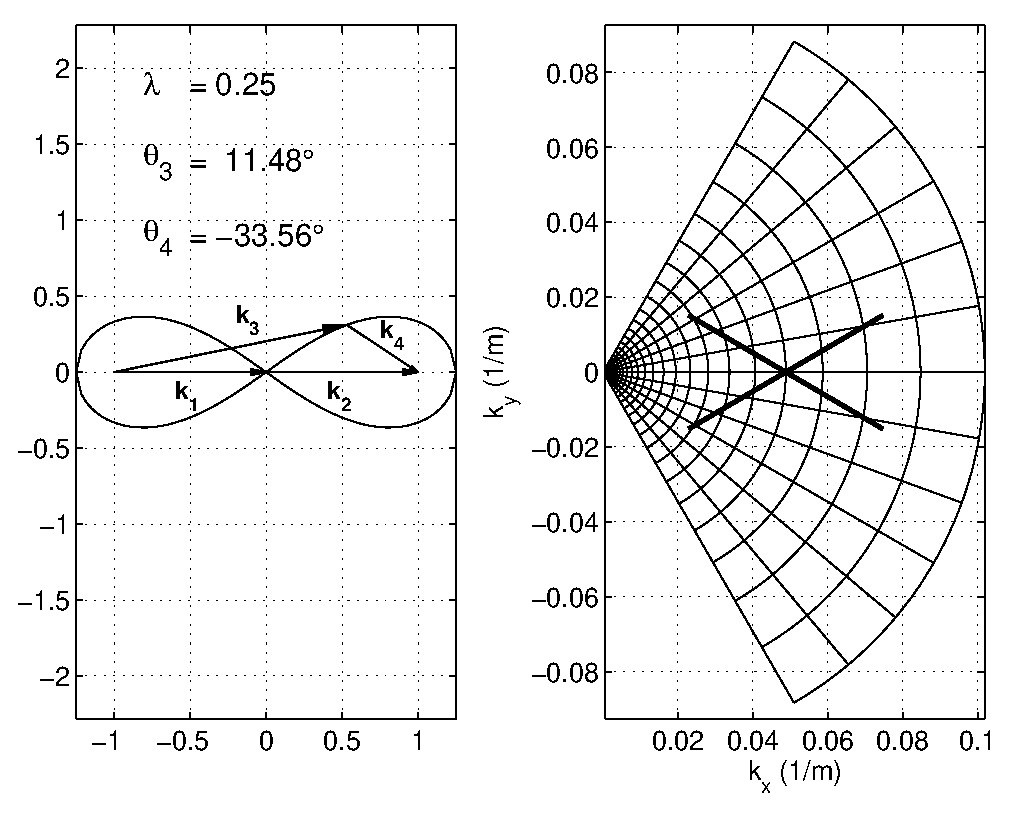
\epsfig{file=config_dia.eps,height=10cm}
              }
      \caption{Wave number configuration for $\lambda$=0.25 and its position in a discrete frequency-
               direction spectrum (from Van Vledder et al., 2000).}
      \label{fig:configdia}
\end{figure}
\\[2ex]
\noindent
Within this discrete interaction approximation, the source term $S_{\rm nl4}(\sigma,\theta)$ for the nonlinear transfer rate is given by:
\begin{equation}
  S_{\rm nl4} (\sigma,\theta) = S^*_{\rm nl4} (\sigma,\theta) + S^{**}_{\rm nl4} (\sigma,\theta)
  \label{eq3-28}
\end{equation}
where $S_{\rm nl4}^{*}$ refers to the first quadruplet and $S_{\rm nl4}^{**}$ to the second quadruplet
(the expressions for $S_{\rm nl4}^{**}$ are identical to those for $S_{\rm nl4}^{*}$ for the mirror directions).
The DIA exchanges wave variance at all three wave number vectors involved in a quadruplet
wave number configuration. The rate of change of wave variance due to the quadruplet
interaction at the three frequency-direction bins can be written as:
\begin{eqnarray}
  \left(
     \begin{array}{l}
        \delta S^*_{\rm nl4} (\sigma,\theta) \\
        \delta S^*_{\rm nl4} (\sigma^+,\theta^+) \\
        \delta S^*_{\rm nl4} (\sigma^-,\theta^-)
     \end{array}
  \right)
  &=&
  \left(
     \begin{array}{c}
        2 \\
       -1 \\
       -1
     \end{array}
  \right)
  C_{\rm nl4} (2\pi)^2 g^{-4} \left(\frac{\sigma}{2\pi} \right)^{11} \times \nonumber \\
  &&\left[E^2 (\sigma,\theta) \left\{\frac{E(\sigma^+,\theta^+)}{(1+\lambda)^4} +
  \frac{E(\sigma^{-},\theta^-)}{(1-\lambda)^4} \right\} \right. \nonumber \\
  &&\left. \left. -2\frac{E(\sigma,\theta) E(\sigma^+,\theta^+) E(\sigma^-,\theta^-)}{(1-\lambda^2)^4}
    \right. \right]
  \label{eq3-30}
\end{eqnarray}
where $C_{nl4} = 3 \times 10^7$ by default.
Eq. (\ref{eq3-30}) conserves wave variance, momentum and
action when the frequencies are geometrically distributed (as is the case in the SWAN
model). The wave variance density at the frequency-direction bins $E(\sigma^+,\theta^+)$ and $E(\sigma^-,\theta^-)$ is
obtained by bi-linear interpolation between the four surrounding frequency-direction bins.
Similarly, the rate of change of variance density is distributed between the four surrounding
bins using the same weights as used for the bi-linear interpolation.
\\[2ex]
\noindent
In the DIA algorithm, Eq. (\ref{eq3-30}) (and its mirror image) is applied to all spectral bins in a
discrete frequency-direction spectrum. Figure~\ref{fig:configdia} shows an example of one wave number
configuration and its mirror image in a discrete spectrum. An extended spectral grid is applied
to compute the interactions in the frequency range affected by the parametric spectral tail.
\\[2ex]
\noindent
SWAN has an option to replace bi-linear interpolation of wave variance density using the
nearest bin approach using a weight equal to 1.
\\[2ex]
\noindent
Following the WAM group (WAMDI, 1988), the quadruplet interaction in shallow water with
depth $d$ is obtained by multiplying the deep water nonlinear transfer rate with a scaling factor
$R(k_pd)$:
\begin{equation}
  S_{\rm nl4}^{\rm finite~depth} = R(k_pd)S_{\rm nl4}^{\rm deep~water}
  \label{eq3-31}
\end{equation}
where $R$ is given by:
\begin{equation}
  R(k_pd) = 1 + \frac{C_{sh1}}{k_pd} (1-C_{sh2}k_pd) e^{C_{sh3}k_pd}
  \label{eq3-32}
\end{equation}
in which $k_p$ is the peak wave number of the frequency spectrum. WAMDI (1988) proposes the
following values of the coefficients:
$C _{sh1}= 5.5$, $C _{sh2} = 5/6$ and $C _{sh3} = -5/4$.
In the shallow water limit, i.e., $k_p \rightarrow 0$ the nonlinear transfer rate tends to infinity. Therefore,
a lower limit of $k_p = 0.5$ is applied, resulting in a maximum value
of $R(k_pd)=4.43$. To increase the model robustness in case of arbitrarily shaped spectra, the peak wave number
$k_p$ is replaced by $k_p = 0.75 \tilde{k}$ (cf. Komen~{\it et~al}., 1994).
\\[2ex]
\noindent
\underline{XNL} \hfill (G. Ph. van Vledder)
\\[2ex]
The second method for calculating the nonlinear interactions in SWAN
is the so-called Webb-Resio-Tracy method (WRT), which is based on the
original six-dimensional Boltzmann integral formulation of
Hasselmann (1962, 1963a,b), and additional considerations by
Webb (1978), Tracy and Resio (1982) and Resio and Perrie (1991).
A detailed description of the WRT method and its implementation in
discrete spectral wave models like SWAN is given in Van Vledder (2006).
An overview of computational methods for computing the exact nonlinear
transfer rate is given in Benoit (2005).
\nocite{Has62,Has63a,Has63b,Web78,Tra82R,Res91P,Vle06,Ben05}
\\[2ex]
\noindent
The Boltzmann integral describes the rate of change of action density
of a particular wave number due to resonant interactions between pairs
of four wave numbers. To interact these wave numbers must satisfy the
following resonance conditions
\begin{equation}
\left .
\begin{array}{ccc}
  \vec{k}_1 + \vec{k}_2 & = & \vec{k}_3 + \vec{k}_4 \\
  \sigma_1 + \sigma_2  & = & \sigma_3 + \sigma_4
\end{array} \:\:\: \right \rbrace \:\:\: .
\label{eq:resonance_2}
\end{equation}
The rate of change of action density $N_1 $ at
wave number $\vec{k}_1$ due to all quadruplet interactions involving
$\vec{k}_1$ is given by
\begin{eqnarray}
\frac{{\partial N_1 }}{{\partial t}} & = & \int\!\!\int\!\!\int G\left( \vec{k}_1
,\vec{k}_2 ,\vec{k}_3 ,\vec{k}_4 \right ) \: \delta \left( \vec{k}_1  + \vec{k}_2  - \vec{k}_3
- \vec{k}_4 \right)
\: \delta \left( {\sigma _1  + \sigma _2  - \sigma _3  - \sigma _4 }
\right) \nonumber \\  & &
\hspace{7mm}\times \:\:\: \left[ {N_1 N_3 \left( {N_4  - N_2 } \right)
+ N_2 N_4 \left(
{N_3  - N_1 } \right)} \right] \: d\vec{k}_2 \: d\vec{k}_3 \: d\vec{k}_4 \:\:\: ,
\end{eqnarray}
where the action density $N$ is defined in terms of the wave number
vector $\vec{k}$, $N = N(\vec{k})$. The term $G$ is a complicated coupling
coefficient for which an explicit expression has been given by Herterich and Hasselmann (1980).
In the WRT method a number of transformations are
made to remove the delta functions. A key element in the WRT method
is to consider the integration space for each ($\vec{k}_1 ,\vec{k}_3$)
combination
\begin{equation}
{{\partial N_1 } \over {\partial t}} = 2\int T\left( {\vec{k}_1 ,\vec{k}_3 }
\right) \: d\vec{k}_3  \:\:\: ,
\end{equation}
in which the function $T$ is given by
\begin{eqnarray}
T \left( \vec{k}_1 ,\vec{k}_3 \right) & = & \int\!\!\int
G\left( \vec{k}_1 ,\vec{k}_2, \vec{k}_3 ,\vec{k}_4 \right) \: \delta \left( \vec{k}_1  +
\vec{k}_2  - \vec{k}_3  - \vec{k}_4 \right) \nonumber \\
& \times & \delta \left( {\sigma _1  + \sigma _2  - \sigma _3  -
\sigma _4 }
\right) \: \theta \left ( \vec{k}_1 , \vec{k}_3 , \vec{k}_4 \right )
\nonumber \\
& \times & \left [ N_1 N_3 \left ( N_4 - N_2 \right ) + N_2 N_4 \left
(
N_3  - N_1 \right ) \right ] \: d\vec{k}_2 \: d\vec{k}_4 \:\:\: ,
\label{eq:WRT_T}
\end{eqnarray}
in which
\begin{equation}
\theta \left( {\vec{k}_1 ,\vec{k}_3 ,\vec{k}_4 } \right) = \left\{ {\begin{array}{*{20}c}
   1 & {\rm{when}} & {\left| {\vec{k}_1  - \vec{k}_3 } \right| \leq \left| {\vec{k}_1  - \vec{k}_4 } \right|}  \\
   0 & {\rm{when}} & {\left| {\vec{k}_1  - \vec{k}_3 } \right| > \left| {\vec{k}_1  - \vec{k}_4 } \right|}  \\
 \end{array} } \right.
\end{equation}
\nocite{Her80H}
\\[2ex]
\noindent
The delta functions in Eq. (\ref{eq:WRT_T}) determine a region in
wave number space along which the integration should be carried out.
The function $\theta$ determines a section of the integral which is
not defined due to the assumption that
$\vec{k}_1$ is closer to $\vec{k}_3$ than $\vec{k}_2$. The crux of the Webb method
consists of using a local co-ordinate system along a so-named
locus, that is, the path in $\vec{k}$ space that satisfies the resonance conditions for a given combination
of $\vec{k}_1$ and $\vec{k}_3$. To that end the $(k_{x},k_{y})$ co-ordinate system is
replaced by a $(s,n)$ co-ordinate system, where $s$ ($n$) is the tangential (normal) direction
along the locus. After some
transformations the transfer integral can then be written as a closed
line integral along the closed locus
\begin{eqnarray}
T \left( \vec{k}_1 ,\vec{k}_3 \right) & = & \oint G \: J
\: \theta ( \vec{k}_1 , \vec{k}_3 , \vec{k}_4 ) \nonumber \\
& \times & \left [ N_1 N_3 \left ( N_4 - N_2 \right ) + N_2 N_4 \left
(
N_3  - N_1 \right ) \right ] \: d s  \:\:\: , \label{eq:WRT_T2}
\end{eqnarray}
in which $G$ is the coupling coefficient and $J$
is the Jacobian term of a function representing the resonance conditions.
The Jacobian term is a function of the group velocities of interacting wave
numbers
\begin{equation}
  J = | \vec{c}_{g,2} - \vec{c}_{g,4}|^{-1}
\end{equation}
Numerically, the Boltzmann integral is computed as the finite sum of
many line integrals $T$ for all discrete combinations of $\vec{k}_1$ and
$\vec{k}_3$. The line integral (\ref{eq:WRT_T2}) is solved by dividing the
locus in typically 40 pieces, such that it's discretized version is
given as:
\begin{equation}
T\left( {\vec{k}_1 ,\vec{k}_3 } \right) \approx \sum_{i=1}^{n_s } G(s_i)
J(s_i) P(s_i) \: \Delta s_i \:\:\: ,
\end{equation}
in which $P(s_i)$ is the product term for a given point on the locus,
$n_s$ is the number of segments, $s_i$ is the discrete co-ordinate
along the locus, and $\Delta s_i$ is the stepsize. Finally, the rate
of change for a given wave number $\vec{k}_1 $ is given by
\begin{equation}
\frac{\partial N(\vec{k}_1)}{\partial t} \approx \sum_{i_{k3}  = 1}^{n_k }
{\sum_{i_{\theta 3}  = 1}^{n_\theta  } T(\vec{k}_1,\vec{k}_3) \: \Delta
k_{i_{k3}} \: \Delta \theta_{i_{\theta 3} } } \label{eq:WRT_numT}
\end{equation}
where $n_k$ and $n_\theta$ are the discrete number of wave numbers and
directions in the computational spectral grid, respectively. Note that although
the spectrum is defined in terms of the vector wave number $\vec{k}$, the
computational grid in a wave model is more conveniently defined in
terms of the absolute wave number and wave direction ($k,\theta$) to
assure directional isotropy of the calculations. Taking all wave
numbers $\vec{k}_1 $ into account produces the complete source term due to
nonlinear quadruplet wave-wave interactions. Details of the
computation of a locus for a given combination of the wave numbers
$\vec{k}_1 $  and $\vec{k}_3 $ can be found in Van Vledder (2006).
\\[2ex]
\noindent
It is noted that these exact interaction calculations are
extremely expensive, typically requiring $10^3$ to $10^4$ times more
computational effort than the DIA. Presently, these calculations can
therefore only be made for highly idealized test cases involving a
limited spatial grid.
\\[2ex]
\noindent
The nonlinear interactions according to the WRT method have been
implemented in SWAN using portable subroutines.
In this implementation, the computational grid of the
WRT method is based to the discrete spectral grid of SWAN.
The WRT method uses a $(\vec{k},\theta)$ grid which is based on the
$(\sigma,\theta)$ grid of SWAN.
In addition, the WRT routines inherit the power of the parametric
spectral tail as in the DIA. Choosing a higher resolution than the computational
grid of SWAN for computing the nonlinear interactions is possible in theory, but this
does not improve the results and is therefore not implemented.
\\[2ex]
\noindent
Because nonlinear quadruplet wave-wave interactions at high
frequencies are important, it is recommended to choose the maximum
frequency of the wave model about six times the peak frequency of the
spectra that are expected to occur in a wave model run. Note that this is important
as the spectral grid determines the range of integration in Eq.~(\ref{eq:WRT_numT}).
The recommended number of frequencies is about 40, with a frequency increment factor
1.07. The recommended directional resolution
for computing the nonlinear interactions is about $10^\circ$. For
specific purposes other resolutions may be used, and some
testing with other resolutions may be needed.
\\[2ex]
\noindent
An important feature of most algorithms for the evaluation of the
Boltzmann integral is that the integration space can be pre-computed.
In the initialization phase of the wave model the
integration space, consisting of the discretized paths of all loci,
together with the interaction coefficients and Jacobians, are
computed and stored in a binary data file. For each discrete water depth such a
data file is generated
and stored in the work directory. The names of these data files
consist of a keyword, "xnl4v5", followed by the keyword "{\it{xxxxx}}", with {\it xxxxx}
the water depth in a certain unit (meters by default), or {\it 99999} for deep water.
The extension of the binary data file is "bqf" (of Binary Quadruplet
File). If a BQF file exists, the program checks if this BQF file has
been generated with the proper spectral grid. If this is not
the case, a new BQF file is generated and the existing BQF file is overwritten.
During a wave model run with various depths, the optimal BQF is
used, by looking at the 'nearest' water depth $d_N$ for which a valid BQF file has been generated.
In addition, the result is rescaled using the DIA scaling (\ref{eq3-32}) according to
\begin{equation}
  S_{\rm nl4}^{d} = S_{\rm nl4}^{d_N} \frac{R(k_pd)}{R(k_pd_N)} \:\:\: .
\end{equation}

\subsubsection{Triads} \label{sec:triad}

The Lumped Triad Approximation (LTA) of Eldeberky (1996), which is a slightly adapted version of the
Discrete Triad Approximation (DTA) of Eldeberky and Battjes (1995) is used in SWAN in each spectral direction:
\begin{equation}
  S_{\rm nl3} (\sigma,\theta) = S^-_{\rm nl3} (\sigma,\theta) + S^+_{\rm nl3} (\sigma,\theta)
  \label{eq3-33}
\end{equation}
with
\begin{equation}
  S^+_{\rm nl3} (\sigma,\theta) = \max [0,\alpha_{\rm EB} 2 \pi c c_g J^2 |\sin\beta| \left \{ E^2(\sigma/2,\theta) -
  2 E(\sigma/2,\theta) E(\sigma,\theta) \right \}]
  \label{eq3-34}
\end{equation}
and
\begin{equation}
  S^-_{\rm nl3} (\sigma,\theta) = -2 S^+_{\rm nl3} (2\sigma,\theta)
  \label{eq3-35}
\end{equation}
in which $\alpha _{\rm EB}$ is a tunable proportionality coefficient. The biphase $\beta$ is approximated with
\begin{equation}
  \beta = -\frac{\pi}{2} + \frac{\pi}{2} \tanh (\frac{0.2}{Ur})
  \label{eq3-36}
\end{equation}
with Ursell number $Ur$:
\begin{equation}
  Ur = \frac{g}{8\sqrt{2} \pi^2} \frac{H_s {T_{m01}}^2}{d^2}
  \label{eq3-37}
\end{equation}
The triad wave-wave interactions are calculated only for $0 \leq Ur \leq 1$. The interaction
coefficient $J$ is taken from Madsen and S{\o}rensen (1993):
\begin{equation}
  J = \frac{k^2_{\sigma/2} (gd + 2 c^2_{\sigma/2})}
           {k_\sigma d (gd + \frac{2}{15} gd^3 k^2_\sigma - \frac{2}{5} \sigma^2 d^2)}
  \label{eq3-38}
\end{equation}

\subsection{First- and second-generation model formulations in SWAN} \label{sec:relaxmod}

The source term $S_{\rm tot}$ for the first- and second-generation formulation (relaxation model) of
SWAN is (Holthuijsen and de Boer, 1988):
\begin{equation}
   S_{\rm tot} =
    \left\{
      \begin{array}{lll}
         S_{\rm in} = A + B E
         \, , & \mbox{if } E < E_{\rm lim} & \mbox{and } |\theta - \theta_w| < \frac{\pi}{2} \\
         \\
         S_{\rm ds,w} = \frac{E_{\rm lim} - E}{\tau}
         \, , & \mbox{if } E > E_{\rm lim} & \mbox{and } |\theta - \theta_w| < \frac{\pi}{2} \\
         \\
         0 \, , & \mbox{if } E > E_{\rm lim} & \mbox{and } |\theta - \theta_w| > \frac{\pi}{2} \\
      \end{array}
    \right.
  \label{eq:relaxmod}
\end{equation}
where $S_{\rm in}$ and $S_{\rm ds,w}$ represent input by wind and decay for over-developed sea states,
respectively, $A$ and $B E$ are a linear and exponential growth term, respectively, $E$ is the
spectral density, $E_{\rm lim}$ is the saturated spectrum, $\tau$ is a time scale and $\theta$ and
$\theta_w$ are the discrete spectral wave direction and the wind direction, respectively.
The expressions for the source terms $S_{\rm in}$ and $S_{\rm ds,w}$ have been modified for shallow water applications
(N. Booij and L.H. Holthuijsen, personal communication, 1996) and are given below.
\nocite{Hol88B}
\\[2ex]
\noindent
The distinction between first- and second-generation is only in the formulation of the
saturated spectrum $E_{\rm lim}$ as outlined below.
\\[2ex]
\noindent
\underline{Linear and exponential growth}\\[2ex]
The linear growth term $A$ is given by  an expression due to Cavaleri and Malanotte-Rizolli
(1981) as adapted by Holthuijsen and de Boer (1988) and Holthuijsen et al. (1996):
\begin{equation}
   A =
    \left\{
      \begin{array}{ll}
         \frac{\beta_1}{2\pi} \frac{\pi}{g^2} C^2_{\rm drag} \left(  \frac{\rho_a}{\rho_w} \right)^2 (U_{10} \max [0,\cos(\theta-\theta_w)])^4
         \, , &  \sigma \geq 0.7 \sigma_{\rm PM,d} \\
         \\
         0 \, , & \sigma < 0.7 \sigma_{\rm PM,d} \\
      \end{array}
    \right.
\end{equation}
where $\beta_1$ is a coefficient that has been tuned to be $\beta_1 = 188$,
$C_{\rm drag}$ is a drag coefficient equal to $C_{\rm drag} = 0.0012$ and
$\sigma_{\rm PM,d}$ is the fully developed peak frequency including the effect of shallow
water and is estimated from the depth dependent
relation of the Shore Protection Manual (1973):
\begin{equation}
  \sigma_{\rm PM,d} = \frac{\sigma_{\rm PM}}{\tanh(0.833 {\tilde d}^{0.375})}
\end{equation}
with the dimensionless depth
\begin{equation}
  {\tilde d} = \frac{gd}{U^2_{10}}
\end{equation}
The Pierson-Moskowitz (1964) frequency is
\begin{equation}
  \sigma_{\rm PM} = \frac{0.13g}{U_{10}} 2\pi
\end{equation}
\nocite{Hol96BB,CER73}
\\[2ex]
\noindent
The exponential growth term $B E$ is due to Snyder et al. (1981) rescaled in terms of $U_{10}$ as
adapted by Holthuijsen and de Boer (1988) and Holthuijsen et al. (1996):
\begin{equation}
  B = \max [0, \beta_2 \frac{5}{2\pi} \frac{\rho_a}{\rho_w} (\frac{U_{10}}{\sigma/k}\cos(\theta-\theta_w) -\beta_3)]\sigma
\end{equation}
in which the coefficients $\beta_2$ and $\beta_3$ have been tuned to be $\beta_2 = 0.59$ and $\beta_3 = 0.12$.
\\[2ex]
\noindent
\underline{Decay}\\[2ex]
If the spectral densities are larger than the wind-dependent saturation spectrum $E_{\rm lim}$, (e.g.,
when the wind decreases), energy is dissipated with a relaxation model:
\begin{equation}
  S_{\rm ds,w} (\sigma,\theta)= \frac{E_{\rm lim}(\sigma,\theta) - E(\sigma,\theta)}{\tau(\sigma)}
\end{equation}
where $\tau(\sigma)$ is a time scale given by
\begin{equation}
  \tau(\sigma) = \beta_4 \left(\frac{2\pi}{\sigma}\right)^2 \frac{g}{U_{10}\cos(\theta - \theta_w)}
\end{equation}
in which the coefficient $\beta_4$ has been tuned to be $\beta_4 = 250$.
\\[2ex]
\noindent
\underline{Saturated spectrum}\\[2ex]
The saturated spectrum has been formulated in term of wave number with a $\cos^2-$directional
distribution centred at the local wind direction $\theta_w$. It is essentially an adapted
Pierson-Moskowitz (1964) spectrum:
\begin{equation}
   S_{\rm tot} =
    \left\{
      \begin{array}{ll}
         \frac{\alpha k^{-3}}{2c_g} \exp{ \left \{ -\frac{5}{4}(\frac{\sigma}{\sigma_{\rm PM,d}})^{-4} \right\} }
         \, \frac{2}{\pi} \, \cos^2(\theta-\theta_w)
         \, , & \mbox{for } |\theta - \theta_w| < \frac{\pi}{2} \\
         \\
         0 \, , & \mbox{for } |\theta - \theta_w| \geq \frac{\pi}{2} \\
      \end{array}
    \right.
\end{equation}
For the \underline{first-generation} formulation, the scale factor $\alpha$ is a constant and equals
\begin{equation}
  \alpha = 0.0081
\end{equation}
For the \underline{second-generation} formulation, the scale factor $\alpha$ depends on the total dimensionless
wave energy ${\tilde E}_{\rm tot,sea}$ of the wind sea part of the spectrum and the dimensionless depth ${\tilde d}$:
\begin{equation}
  \alpha = \max [ (0.0081 + (0.013 - 0.0081)e^{-{\tilde d}}), 0.0023 {\tilde E}^{-0.223}_{\rm tot,sea} ]
\end{equation}
where the total dimensionless wind sea wave energy ${\tilde E}_{\rm tot,sea}$ is given by:
\begin{equation}
  {\tilde E}_{\rm tot,sea} = \frac{g^2 E_{\rm tot,sea}}{U^4_{10}}
\end{equation}
with
\begin{equation}
  E_{\rm tot,sea} = \int_{\theta_w - \pi/2}^{\theta_w + \pi/2} \int_{0.7 \sigma_{\rm PM,d}}^{\infty}
  E(\sigma,\theta) d\sigma d\theta
\end{equation}
The maximum value of $\alpha$ is taken to be 0.155. This dependency of $\alpha$ on the local
dimensionless energy of the wind sea permits an overshoot in the wave spectrum under wave
generation conditions. For deep water $\alpha = 0.0081$ as proposed by Pierson and Moskowitz (1964).

\section{Wave damping due to vegetation} \label{sec:veget}

Apart from the six processes as outlined in Section~\ref{sec:soursnk}, SWAN has an option to include
wave damping over a vegetation field (mangroves, salt marshes, etc.) at variable depths.
A popular method of expressing the wave dissipation due to vegetation is the cylinder approach
as suggested by Dalrymple~{\it et~al}. (1984). Here,
energy losses are calculated as actual work carried out by the vegetation due to plant
induced forces acting on the fluid, expressed in terms of a Morison type equation.
In this method, vegetation motion such as vibration due to vortices and swaying is
neglected. For relatively stiff plants the drag force is considered dominant and inertial
forces are neglected. Moreover, since the drag due to friction is much smaller than the
drag due to pressure differences, only the latter is considered. Based on
this approach, the time-averaged rate of energy dissipation per unit
area over the entire height of the vegetation is given by:
\begin{equation}
  \varepsilon_{\rm v} = \frac{2}{3\pi} \rho C_{\rm D} b_{\rm v} N_{\rm v} \left( \frac{gk}{2\sigma} \right)^3
                 \frac{\sinh^3 k\alpha h + 3\sinh\, k\alpha h}{3k\cosh^3 kh} H^3
\end{equation}
where $\rho$ is the water density, $C_{\rm D}$ is the drag coefficient, $b_{\rm v}$ is the
stem diameter of cylinder (plant), $N_{\rm v}$ is the number of plants per square meter,
$\alpha h$ is the vegetation height, $h$ is the water depth and $H$ is the wave height.
This formula was modified by Mendez and Losada (2004) for irregular waves.
The mean rate of energy dissipation per unit horizontal
area due to wave damping by vegetation is given by:
\begin{equation}
  <\varepsilon_{\rm v}> = \frac{1}{2\sqrt{\pi}} \rho {\tilde C}_{\rm D} b_{\rm v} N_{\rm v} \left( \frac{gk}{2\sigma} \right)^3
                   \frac{\sinh^3 k\alpha h + 3\sinh\, k\alpha h}{3k\cosh^3 kh} H_{\rm rms}^3
  \label{eq:mendez}
\end{equation}
with ${\tilde C}_{\rm D}$ is the bulk drag coefficient that may depend on the wave height. This is the only
calibration parameter required for a given plant type.
\nocite{Dal84KH,Men04L}
\\[2ex]
\noindent
To include wave damping due to vegetation in SWAN, Eq.~(\ref{eq:source}) will be extended with $S_{\rm ds,veg}$ based
on Eq.~(\ref{eq:mendez}). A spectral version of the vegetation dissipation model of Mendez and
Losada can be obtained by expanding Eq.~(\ref{eq:mendez}) to include frequencies and directions as
follows
\begin{equation}
  S_{\rm ds,veg} (\sigma,\theta) = \frac{D_{\rm tot}}{E_{\rm tot}} E(\sigma,\theta)
\end{equation}
with
\begin{equation}
  D_{\rm tot} = -\frac{1}{2g\sqrt{\pi}} {\tilde C}_{\rm D} b_{\rm v} N_{\rm v} \left( \frac{g{\tilde{k}}}{2{\tilde{\sigma}}} \right)^3
                   \frac{\sinh^3 {\tilde{k}}\alpha h + 3\sinh\, {\tilde{k}}\alpha h}{3k\cosh^3 {\tilde{k}}h} H_{\rm rms}^3
  \label{eq:mendez2}
\end{equation}
where the mean frequency $\tilde{\sigma}$, the mean wave number $\tilde{k}$ are given by Eqs.~(\ref{eq3-14}) and (\ref{eq3-15}), respectively.
With $H^2_{\rm rms} = 8E_{\rm tot}$, the final expression reads
\begin{equation}
  S_{\rm ds,veg} = -\sqrt{\frac{2}{\pi}} g^2 {\tilde C}_{\rm D} b_{\rm v} N_{\rm v} \left( \frac{{\tilde{k}}}{{\tilde{\sigma}}} \right)^3
                   \frac{\sinh^3 {\tilde{k}}\alpha h + 3\sinh\, {\tilde{k}}\alpha h}{3k\cosh^3 {\tilde{k}}h} \sqrt{E_{\rm tot}} E(\sigma,\theta)
\end{equation}
\\[2ex]
\noindent
Apart from extending the Mendez and Losada's formulation to a full
spectrum, the possibility to vary the vegetation vertically is included. The
contribution of each vertical segment is calculated individually with the total energy
dissipation equal to the sum of the dissipation in each layer up till the still water level.
With this implementation of the differences in characteristics of each layer, plants such
as mangrove trees may be conveniently input into the SWAN model. The layer-wise
segmentation is implemented by integration of the energy dissipation over
height as follows:
\begin{equation}
  S_{\rm ds,veg} = \sum_{i=1}^{I} S_{{\rm ds,veg},i}
\end{equation}
where $I$ the number of vegetation
layers and $i$ the layer under consideration with the energy dissipation for layer $i$.
First, a check is performed to establish whether the vegetation is emergent or submergent
relative to the water depth. In case of submergent vegetation the energy contributions of
each layer are added up for the entire vegetation height. In case of emergent vegetation
only the contributions of the layers below the still water level are taken into account.
The implementation of vertical variation is illustrated in Figure~\ref{fig:veglay}.
The energy dissipation term for a given layer $i$ therefore becomes
\begin{eqnarray}
  &&S_{{\rm ds,veg},i} = -\sqrt{\frac{2}{\pi}} g^2 {\tilde C}_{{\rm D},i} b_{{\rm v},i} N_{{\rm v},i} \left( \frac{{\tilde{k}}}{{\tilde{\sigma}}} \right)^3
                   \sqrt{E_{\rm tot}} \nonumber \\
                   &&\frac{\left(\sinh^3 {\tilde{k}}\alpha_i h - \sinh^3 {\tilde{k}}\alpha_{i-1} h\right) +
                    3\left( \sinh\, {\tilde{k}}\alpha_i h - \sinh\, {\tilde{k}}\alpha_{i-1} h\right)}
                   {3k\cosh^3 {\tilde{k}}h} E(\sigma,\theta)
\end{eqnarray}
The corresponding terms for each layer can then be added and the total integrated as
described earlier to obtain the energy dissipation over the entire spectrum.
Here $h$ is the total water depth and $\alpha_i$ the ratio of the depth of the layer under
consideration to the total water depth up to the still water level, such that
\begin{equation}
  \sum_{i=1}^{I} \alpha_i \leq 1
\end{equation}
\begin{figure}[htb]
   \centerline{
      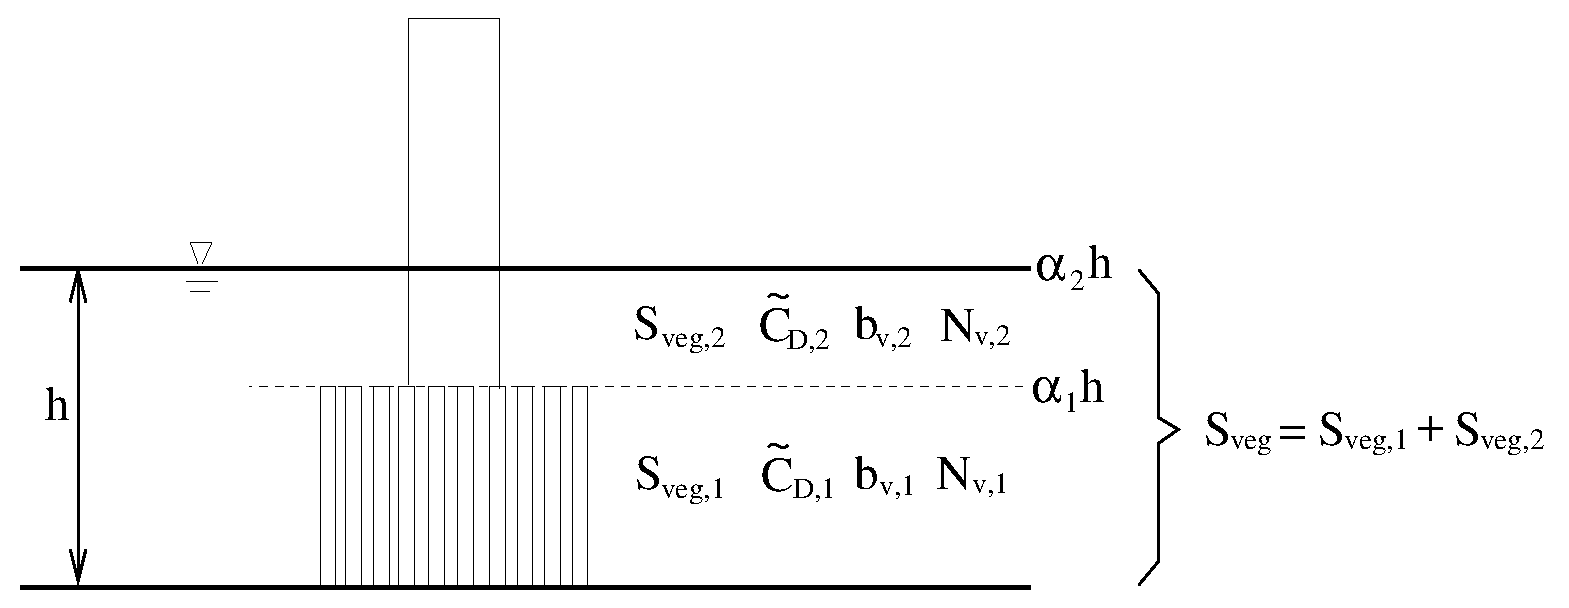
\epsfig{file=veglay.eps,height=5cm}
              }
      \caption{Layer schematization for vegetation.}
      \label{fig:veglay}
\end{figure}
\\[2ex]
\noindent
Finally, in addition to the vertical variation, the possibility of horizontal variation of the
vegetation characteristics is included as well. This inclusion enables the vegetation in a
given region to be varied so as to reflect real density variations in the field.

\section{The influence of ambient current on waves} \label{sec:curre}

Waves are subject to the influence of ambient current, when they propagate on it. The ambient current
can be tidal current, ocean current, local wind generated current, river current and wave generated
current. It has been observed that current affects the growth and decay of waves (Yu, 1952;
Hedges~{\it et~al}., 1985; Lia~{\it et~al}., 1989). The observations have shown that in a strong opposite
current the wave steepness and wave height increase significantly. These changes take place rapidly
where the waves are blocked by the current, often accompanied with current-induced whitecapping and wave
reflections. Moreover, at the blocking frequency action is also partially transferred away from the blocking
frequency to higher and lower frequencies by nonlinear wave-wave interactions (Ris, 1997).
\\[2ex]
\noindent
It was Longuet-Higgins and Stewart (1960, 1961, 1962) who founded the theoretical description of wave-current
interactions. Since then, many additional results of wave-current interactions have been published. If waves
propagate in the presence of ambient current, action density is conserved whereas energy density is not.
Therefore, in SWAN the action balance equation has been adopted.

\section{Modelling of obstacles} \label{sec:obstac}

SWAN can estimate wave transmission through a (line-)structure such as a breakwater (dam).
It is assumed that the obstacle is narrow compared to the grid size.
If in reality the width is large compared with grid size,
the feature preferably is to be modeled as a bathymetric feature.
The following text refers to narrow obstacles.
\\[2ex]
\noindent
Such an obstacle will affect the wave field in three ways:
\begin{itemize}
  \item it will reduce the wave height of waves propagating through or over the obstacle all along its length,
  \item it will cause waves to be reflected, and
  \item it will cause diffraction around its end(s).
\end{itemize}
In irregular, short-crested wave fields, however, it seems that the effect of diffraction is small, except in a
region less than one or two wavelengths away from the tip of the obstacle (Booij~{\it et~al}., 1993). Therefore
the model can reasonably account for waves around an obstacle if the directional spectrum of incoming
waves is not too narrow, unless one is interested in the wave field deep into the shadow zone.
\\[2ex]
\noindent
Since obstacles usually have a transversal area that is too small to be resolved
by the bottom grid in SWAN, an obstacle is modelled as a line in the computational area. See Section~\ref{sec:numobst}
for the numerical implementation of obstacles in SWAN.

\subsection{Transmission}

There are several mechanisms for transmission of waves. In SWAN, the user may compute transmission of waves passing
over a dam with a closed surface or may choose a constant transmission coefficient.
\\[2ex]
\noindent
If the crest of the breakwater is at a level
where (at least part of the) waves can pass over, the transmission coefficient $K_{t}$ (defined as the ratio of
the (significant) wave height at the downwave side of the dam over the (significant) wave height at the
upwave side) is a function of wave height and the difference in crest level and water level. It must be noted that
the transmission coefficient can never be smaller than 0 or larger than 1. In SWAN, two expressions
can be employed. The first is taken from Goda~{\it et~al}. (1967):
\begin{equation}
  K_t =
    \left\{
      \begin{array}{ll}
         1 \, , & \frac{F}{H_i} < -\beta - \alpha \\
         0.5 (1 - \sin(\frac{\pi}{2\alpha}(\frac{F}{H_i}+\beta)))\, , & -\beta -\alpha \leq \frac{F}{H_i} \leq \alpha - \beta \\
         0 \, , & \frac{F}{H_i} > \alpha - \beta
      \end{array}
    \right.
  \label{eq2-9}
\end{equation}
where $F=h-d$ is the freeboard of the dam and where $H_i$ is the incident (significant) wave height at the
upwave side of the obstacle (dam), $h$ is the crest level of the dam above the reference level (same as
reference level of the bottom), $d$ the mean water level relative to the reference level, and the coefficients
$\alpha$, $\beta$ depend on the shape of the dam (Seelig, 1979) as given in Table~\ref{tab:see79}. It should be
noted that this formula is only valid for slopes more gentle than 1:0.7 (1.4:1 or 55 degrees).
\begin{table}[htb]
\begin{center}
\caption{Parameters for transmission according to Goda~{\it et~al}. (1967).}
\label{tab:see79}
\begin{tabular}{l c c}
\hline
  case & $\alpha$ & $\beta$ \\
\hline
    vertical thin wall   & 1.8 & 0.1  \\
    caisson              & 2.2 & 0.4  \\
    dam with slope 1:3/2 & 2.6 & 0.15 \\
\hline
\end{tabular}
\end{center}
\end{table}
Expression (\ref{eq2-9}) is based on experiments in a wave flume, so strictly speaking it is only valid for
normal incidence waves. Since there are no data available on oblique waves, it is assumed that the
transmission coefficient does not depend on direction. Furthermore, it is assumed that the frequencies remain
unchanged over an obstacle (only the energy scale of the spectrum is affected and not the spectral shape).
\\[2ex]
\noindent
For an impermeable rough low-crested dam, the following expression of d'Angremond~{\it et~al} (1996) is chosen:
\begin{equation}
  K_t = -0.4 \frac{F}{H_i} + 0.64 (\frac{B_k}{H_i})^{-0.31} (1 - e^{-0.5{\xi}_p})
  \label{eq:dangremond}
\end{equation}
with $B_k$ the crest width and ${\xi}_p \equiv \tan \alpha/\sqrt{H_i/L_{0p}}$ the breaker parameter. For this,
the slope of the breakwater $\alpha$ must be given and $L_{0p} = g T_p^2/ 2\pi$ is the deep water wave length.
The restriction to eq. (\ref{eq:dangremond}) is as follows:
\begin{equation}
  0.075 \leq K_t \leq 0.9
\end{equation}
In most cases, the crest width is such that $B_k < 10 H_i$. However, if this is not the case, the following expression
should be used instead of (\ref{eq:dangremond}):
\begin{equation}
  K_t = -0.35 \frac{F}{H_i} + 0.51 (\frac{B_k}{H_i})^{-0.65} (1 - e^{-0.41{\xi}_p})
  \label{eq:dangremond2}
\end{equation}
with the restriction:
\begin{equation}
  0.05 \leq K_t \leq -0.006\frac{B_k}{H_i} + 0.93
\end{equation}
The formula's (\ref{eq:dangremond}) and (\ref{eq:dangremond2}) give a discontinuity at $B_k = 10 H_i$. Following
Van der Meer~{\it et~al} (2005), for practical
application, Eq. (\ref{eq:dangremond}) is applied if $B_k < 8 H_i$, Eq. (\ref{eq:dangremond2}) if $B_k > 12 H_i$ and
in between ($8 H_i \leq B_k \leq 12 H_i$), a linear interpolation is carried out.
\nocite{God67TM,See79,Dan96MJ,Mee05BZW}

\subsection{Reflection}

Often there is reflection against quays or breakwaters.
Depending on the nature of the obstacle (a smooth surface or a rubble-mound breakwater)
the reflected wave field can be more or less scattered.
SWAN is able to diffuse the reflection over wave components in different directions.

\subsection{Diffraction} \label{sec:diffrac}

To accommodate diffraction in SWAN simulations, a phase-decoupled refraction-diffraction approximation
is suggested (Holthuijsen~{\it et~al}., 2003). It is expressed in terms of the directional turning rate
of the individual wave components in the 2D wave spectrum. The approximation is based on the mild-slope
equation for refraction and diffraction, omitting phase information. It does therefore not permit coherent
wave fields in the computational domain.
\\[2ex]
\noindent
In a simplest case, we assume there are no currents. This means that $c_\sigma = 0$. Let denotes the
propagation velocities in geographic and spectral spaces for the situation without diffraction as:
$c_{x,0}$, $c_{y,0}$ and $c_{\theta,0}$. These are given by:
\begin{equation}
  c_{x,0} = \frac{\partial \omega}{\partial k} \cos\theta\,,
  c_{y,0} = \frac{\partial \omega}{\partial k} \sin\theta\,,
  c_{\theta,0} = -\frac{1}{k}\frac{\partial \omega}{\partial h} \frac{\partial h}{\partial n}
  \label{eq3-42}
\end{equation}
where $k$ is the wave number and $n$ is perpendicular to the wave ray. We consider the following eikonal
equation
\begin{equation}
  K^2 = k^2 (1+\delta)
  \label{eq3-43}
\end{equation}
with $\delta$ denoting the diffraction parameter as given by:
\begin{equation}
  \delta = \frac{\nabla (c c_g \nabla \sqrt{E})}{c c_g \sqrt{E}}
  \label{eq3-44}
\end{equation}
where $E(x,y)$ is the total energy of the wave field ($\sim H^2_s$).
Due to diffraction, the propagation velocities are given by:
\begin{equation}
  c_x = c_{x,0} \overline{\delta}\,,
  c_y = c_{y,0} \overline{\delta}\,,
  c_\theta = c_{\theta,0} \overline{\delta} - \frac{\partial \overline{\delta}}{\partial x}
   c_{y,0} + \frac{\partial \overline{\delta}}{\partial y}c_{x,0}
  \label{eq3-45}
\end{equation}
where
\begin{equation}
  \overline{\delta} = \sqrt{1+\delta}
  \label{eq3-46}
\end{equation}
\\[2ex]
\noindent
In early computations, the wave fields often showed slight wiggles in geographic space with a wavelength
of about 2$\Delta x$ in $x-$direction. These unduly affected the estimations of the gradients that were
needed to compute the diffraction parameter $\delta$. The wave field was therefore smoothed with the following
convolution filter:
\begin{equation}
  E_{i,j}^n = E_{i,j}^{n-1} - 0.2 [E_{i-1,j}+E_{i,j-1}-4E_{i,j}+E_{i+1,j}+E_{i,j+1}]^{n-1}
\end{equation}
where $i,j$ is a grid point and the superscript $n$ indicates iteration number of the convolution cycle.
The width of this filter (standard deviation) in $x-$direction $\varepsilon_x$, when applied $n$ times is
\begin{equation}
  \varepsilon_x \approx \frac{1}{2} \sqrt{3n} \Delta x
\end{equation}
By means of computations, $n=6$ is found to be an optimum value (corresponding to spatial resolution of
1/5 to 1/10 of the wavelength), so that $\varepsilon_x \approx 2\Delta x$. For the $y-$direction, the expressions
are identical, with $y$ replacing $x$. Note that this smoothing is only applied to compute the diffraction
parameter $\delta$. For all other computations the wave field is not smoothed.
\\[2ex]
\noindent
Diffraction is SWAN should \underline{not} be used if,
\begin{itemize}
  \item an obstacle or coastline covers a significant part of the down-wave view, \underline{and}
  \item the distance to that obstacle or coastline is small (less than a few wavelengths), \underline{and}
  \item the reflection off that obstacle or coastline is coherent, \underline{and}
  \item the reflection coefficient is significant.
\end{itemize}
This implies that the SWAN diffraction approximation can be used in most situations near absorbing or reflecting
coastlines of oceans, seas, bays, lagoons and fjords with an occasional obstacle such as islinds, breakwaters,
or headlands but \underline{NOT} in harbours or in front of reflecting breakwaters or near wall-defined
cliff walls. Behind breakwaters (which may be reflecting), the SWAN results seem reasonable if the above
conditions are met.

\section{Wave-induced set-up} \label{sec:setup}

In a (geographic) 1D case the computation of the wave-induced set-up is based on the vertically integrated
momentum balance equation which is a balance between the wave force (gradient of the wave radiation
stress normal to the coast) and the hydrostatic pressure gradient (note that the component parallel to the
coast causes wave-induced currents but no set-up).
\begin{equation}
  \frac{dS_{xx}}{dx} + \rho g H \frac{d \overline{\eta}}{dx} = 0
  \label{eq3-39}
\end{equation}
where $d$ is the total water depth (including the wave-induced set-up) and $\eta$ is the mean surface elevation
(including the wave-induced set-up) and
\begin{equation}
   S_{xx} = \rho g \int [n \cos^2 \theta + n - \frac{1}{2}]E d \sigma d\theta
  \label{eq3-40}
\end{equation}
is the radiation stress tensor.
\\[2ex]
\noindent
Observation and computations based on the vertically integrated momentum balance equation of
Dingemans~{\it et~al}. (1987) show that the wave-induced currents are mainly driven by the divergence-free
part of the wave forces whereas the set-up is mainly due to the rotation-free part of these forces. To
compute the set-up in 2D, it would then be sufficient to consider the divergence of the momentum balance
equation. If the divergence of the acceleration in the resulting equation is ignored, the result is:
\begin{equation}
  \frac{\partial F_x}{\partial x} + \frac{\partial F_y}{\partial y} -
  \frac{\partial}{\partial x} (\rho g H \frac{\partial \overline{\eta}}{\partial x}) -
  \frac{\partial}{\partial y} (\rho g H \frac{\partial \overline{\eta}}{\partial y}) = 0
  \label{eq3-41}
\end{equation}
This approximation can \underline{only} be applied to open coast (unlimited supply of water from outside
the domain, e.g. nearshore coasts and estuaries) in contrast to closed basin, e.g. lakes, where this approach
should not be used.

\chap{Numerical approaches} \label{ch:numerics}

\section{Introduction} \label{sec:intnum}

The accuracy with which
physical processes for wave growth are approximated numerically is of crucial importance in assessing the
predictive realism of spectral wave models. There is a
need to separate these numerical errors from errors due to physical modelling.
Third-generation wave models pose a numerical difficulty caused by the presence of
multiple time scales. This is
a reflection of the physical nature of wind waves, which consist of a wide
range of frequencies. The ratio of the largest to the smallest time scale of spectral components is often substantially
larger than one. When this is the case, the action balance equation is called stiff
(Press~{\it et~al}., 1993)\footnote{The equivalent situation for such an equation is to have eigenvalues
of very different magnitudes.}. Taking proper account of these time scales is a
necessary condition for numerical accuracy. This would require
the use of a very small time step in a numerical algorithm, which may be
impractical. Moreover, the action balance equation is usually so
stiff that its numerical implementation combined with economically large
time steps often prevent a stable solution. In this respect, nonlinear four-wave interaction
usually poses the biggest problem, since this process is associated with
high sensitivity to spectral change.
\\[2ex]
\noindent
In a number of papers concerning spectral wave computation, numerical measures are proposed to achieve stable model
results economically.
WAMDI Group (1988) suggest to use a semi-implicit time integration scheme with a time step that matches the time scale of
low-frequency waves.
However, numerically stable solution of the resulting sytem of equations can not be guaranteed
(Hargreaves and Annan, 2001).
The ratio of the largest eigenvalue to the smallest eigenvalue of the stiff system
of equations, called the condition number, can be so large that even a fully-implicit method combined with large
time steps precludes a stable solution. For counterexamples, see Hargreaves and Annan (2001).
The only remedy is time step reduction or under-relaxation so that the modified system of
equations has a spectrum of eigenvalues with a more favourable condition number.
\nocite{Har01A}
\\[2ex]
\noindent
To guarantee numerical stability at relatively large time steps, the so-called action density limiter has been introduced
in WAM in the early 1980's (Hersbach and Janssen, 1999). This limiter restricts the rate of change of the energy
spectrum at each time step. Because low-frequency waves
carry the most energy, it is desirable to solve the balance equation in this
part of the spectrum accurately without intervention by the limiter, whereas
for high-frequency waves using an equilibrium level is sufficient. Although this approach lacks a rigorous
foundation and is not generally applicable or valid, it appears to
guarantee numerical stability at relatively large time steps even when these
do not match the time scales of wave growth. Moreover, it is believed that
the limiter will not affect the stationary solution when convergence is
reached. This assumption is widely employed as a justification for the use of
limiters. For an overview, we refer to Hersbach and Janssen (1999) and
Tolman (2002) and the references quoted therein.
Tolman (1992) proposes an alternative to the action
density limiter in which the time step is
dynamically adjusted where necessary to ensure accurate wave evolution. The calculation of
this optimal time step is related to the action density limiter. Further details can be
found in Tolman (1992, 2002).
\nocite{Her99J,Tol02}.
\\[2ex]
\noindent
The steady-state solution in the SWAN model is obtained in an iterative manner,
which can be regarded as a time marching method
with a pseudo time step.
This pseudo time step generally does not match the relatively small time scale in frequency space
and consequently, divergence will occur.
Therefore, SWAN makes use of the action density limiter to stabilize the iteration process
(Booij~{\it et~al}., 1999). However, experience with SWAN has revealed that
the limiter acts not only in the equilibrium space, but also in the energy-containing part of the
wave spectrum. This finding is also confirmed by Tolman (2002). Furthermore, the
limiter appears to be active over almost all spectra in the geographical domain
and during the entire iteration process. This activity has been associated
with poor convergence behaviour, such as small-amplitude oscillation in frequency space. Ris
(1999) demonstrated that stationary SWAN results are influenced by the settings of the action
limiter while De Waal (2001) suspects that the limiter acts as a hidden sink
in the source term balance under equilibrium conditions. The question to
what extent this limiter adversely affects the stationary solution of SWAN has not
been addressed previously, and is considered here.
\nocite{Boo99RH,Tol02,Ris99,DeW01}
\\[2ex]
\noindent
An alternative way to restrict the high rate of change
at higher frequencies is under-relaxation, i.e. making smaller updates by means
of a much smaller (pseudo) time step (Ferziger and Peri\'{c}, 1999).
Consequently, a limiter may no longer be needed. Although this
approach may be suitable to SWAN, it slows down convergence significantly.
Here, we propose a new method that finds a
compromise between fast convergence on the one hand and minimizing the role of the limiter in the
energetic part of the
spectrum on the other. The key idea to achieve this is to link the extent of updating to the wave
frequency---the
larger the frequency, the smaller the update. This approach is therefore called frequency-dependent
under-relaxation.
\nocite{Fer99P}
\\[2ex]
\noindent
The second objective concerns the formulation and the use of termination criteria required by
the iteration procedure in SWAN.
In principle, the iterative process should be stopped if the convergence error defined as the
difference between the current iterate and the stationary solution is smaller
than a prescribed tolerance. At present, the stopping criteria in SWAN make
use of the difference between successive iterates as a measure of the error
in the converged solution.
Experiences in the application of SWAN have shown that the iteration process is often
more erratic and typically much slower than reported by Booij~{\it et~al}. (1999).
As a result, the current stopping criteria
often lead to premature termination of simulations. This is characterised by the fact that,
due to the relatively low rate of convergence,
the convergence error is larger than the difference between the successive iterates.
A stopping criterion is proposed that uses the second derivative
or curvature of the series of successive iterates of the calculated wave height. The premise is that
this curvature approaches zero upon full convergence.
\nocite{Boo99RH}

\section{Discretization} \label{sec:dsc}

Discretization of (\ref{eq:actbal2}) is carried out using the finite difference method.
The homogeneous part of equation (\ref{eq:actbal2}) is given by
\begin{equation}
  \frac{\partial N}{\partial t} +
  \frac{\partial c_x N}{\partial x} +
  \frac{\partial c_y N}{\partial y} +
  \frac{\partial c_\sigma N}{\partial \sigma} +
  \frac{\partial c_\theta N}{\partial \theta}\, .
  \label{eq:acthom}
\end{equation}
We choose a rectangular grid with constant mesh sizes $\Delta x$ and $\Delta y$ in $x-$ and $y-$direction,
respectively. The spectral space is divided into elementary bins with a constant directional
resolution $\Delta \theta$ and a constant relative frequency resolution $\Delta \sigma/\sigma$
(resulting in a logarithmic frequency distribution). We denote the grid counters as $1 \leq i \leq N_x$,
$1 \leq j \leq N_y$, $1 \leq l \leq N_{\sigma}$ and $1 \leq m \leq N_{\theta}$ in $x-$, $y-$, $\sigma-$
and $\theta-$spaces, respectively. All variables are located at points $(i,j,l,m)$. Time discretization
takes place with the implicit Euler technique. We obtain the following approximation of~(\ref{eq:acthom}):
\begin{eqnarray}
    \frac{N^{n}-N^{n-1}}{\Delta t}|_{i,j,l,m} &+&
    \frac{[c_x N]_{i+1/2}-[c_x N]_{i-1/2}}{\Delta x}|^{n}_{j,l,m} + \nonumber \\
  &&\frac{[c_y N]_{j+1/2}-[c_y N]_{j-1/2}}{\Delta y}|^{n}_{i,l,m} + \nonumber \\
  &&\frac{[c_\sigma N]_{l+1/2}-[c_\sigma N]_{l-1/2}}{\Delta \sigma}|^{n}_{i,j,m} + \nonumber \\
  &&\frac{[c_\theta N]_{m+1/2}-[c_\theta N]_{m-1/2}}{\Delta \theta}|^{n}_{i,j,l}\, ,
  \label{eq:actdisc}
\end{eqnarray}
where $n$ is a time-level with $\Delta t$ a time step. Note that locations in between consecutive
counters are reflected with the half-indices.

\subsection{Discretization in geographical space}

Since, the unknown $N$ and the propagation velocities are only given in points $(i,j,l,m)$,
further approximation is needed. A first order upwind scheme
in geographical space may be employed, since it fully
monotone, i.e. it can not to give rise to spurious oscillations.
A disadvantage of this scheme is that it is numerically
diffusive, which naturally degrades the accuracy of the model.
This numerical diffusion is caused by gradients of wave action across geographic space, e.g. due to refraction by bathymetry or currents.
However, in
the current SWAN version, two alternatives to this scheme are implemented, namely the second
order SORDUP and the third order Stelling/Leendertse schemes. These schemes produce far less numerical diffusion.
\\[2ex]
\noindent
\underline {First order upwind scheme; BSBT}
\\[2ex]
\noindent
The fluxes $c_x N$ at $(i+1/2,j,l,m)$ and $c_y N$ at $(i,j+1/2,l,m)$ are approximated in the
following way:
\begin{equation}
  c_x N|_{i+1/2,j,l,m} = \left\{
                           \begin{array}{l}
                              c_x N|_{i,j,l,m}\,, \qquad c_x|_{i,j,l,m} > 0 \\
                              c_x N|_{i+1,j,l,m}\,, \quad c_x|_{i+1,j,l,m} < 0
                           \end{array}
                         \right.
  \label{eq:fluxx}
\end{equation}
and
\begin{equation}
  c_y N|_{i,j+1/2,l,m} = \left\{
                           \begin{array}{l}
                              c_y N|_{i,j,l,m}\,, \qquad c_y|_{i,j,l,m} > 0 \\
                              c_y N|_{i,j+1,l,m}\,, \quad c_y|_{i,j+1,l,m} < 0
                           \end{array}
                         \right.\, .
  \label{eq:fluxy}
\end{equation}
The fluxes at $(i-1/2,j,l,m)$ and $(i,j-1/2,l,m)$ are obtained from (\ref{eq:fluxx}) and (\ref{eq:fluxy}),
respectively, by decreasing the indices by 1 in appropriate manner. Note that the combination of the time
and geographic space discretizations in (\ref{eq:actdisc}), (\ref{eq:fluxx}) and (\ref{eq:fluxy}) is also
known as the first order, backward space, backward time (BSBT) scheme.
\\[2ex]
\noindent
\underline {SORDUP}
\\[2ex]
\noindent
For the SORDUP scheme which is the \underline{default scheme for stationary computations}, the two terms in
Eqs. (\ref{eq:fluxx}) and (\ref{eq:fluxy}) representing $x-$ and $y-$derivatives are replaced by
\begin{equation}
  \left( \frac{1.5 (c_x N)_{i_x} - 2 (c_x N)_{i_x-1} + 0.5 (c_x N)_{i_x-2}}{\Delta x} \right)^{i_t,n}_{i_y, i_{\sigma}, i_{\theta}}
\end{equation}
and
\begin{equation}
  \left( \frac{1.5 (c_y N)_{i_y} - 2 (c_y N)_{i_y-1} + 0.5 (c_y N)_{i_y-2}}{\Delta y} \right)^{i_t,n}_{i_x, i_{\sigma}, i_{\theta}}
\end{equation}
See also Rogers~{\it et~al}. (2002).
In the neighboorhood of open boundaries, land boundaries and obstacles (i.e., the last two grids adjoining such grid points for
the SORDUP scheme), SWAN will revert to the first order upwind BSBT scheme. This scheme has a larger numerical diffusion but that
is usually acceptable over the small distances involved.
\\[2ex]
\noindent
\underline{Stelling and Leendertse scheme}
\\[2ex]
\noindent
For the Stelling and Leendertse scheme which is the \underline{default scheme for nonstationary computations}, the two terms in
Eqs. (\ref{eq:fluxx}) and (\ref{eq:fluxy}) representing $x-$ and $y-$derivatives are replaced by
\begin{equation}
  \left( \frac{\frac{5}{6} (c_x N)_{i_x} - \frac{5}{4} (c_x N)_{i_x-1} + \frac{1}{2} (c_x N)_{i_x-2} \frac{1}{12} (c_x N)_{i_x-3}}{\Delta x} \right)^{i_t,n}_{i_y, i_{\sigma}, i_{\theta}}
  + \left( \frac{(c_x N)_{i_x+1} - (c_x N)_{i_x-1}}{4 \Delta x} \right)^{i_t-1}_{i_y, i_{\sigma}, i_{\theta}}
\end{equation}
and
\begin{equation}
  \left( \frac{\frac{5}{6} (c_y N)_{i_y} - \frac{5}{4} (c_y N)_{i_y-1} + \frac{1}{2} (c_y N)_{i_y-2} \frac{1}{12} (c_y N)_{i_y-3}}{\Delta y} \right)^{i_t,n}_{i_x, i_{\sigma}, i_{\theta}}
  + \left( \frac{(c_y N)_{i_y+1} - (c_y N)_{i_y-1}}{4 \Delta y} \right)^{i_t-1}_{i_x, i_{\sigma}, i_{\theta}}
\end{equation}
See also Stelling and Leendertse (1992).
In the neighboorhood of open boundaries, land boundaries and obstacles (i.e., the last three grids adjoining such grid points for
the Stelling and Leendertse scheme), SWAN will revert to the first order upwind BSBT scheme.
\\[2ex]
\noindent
Usually, the numerical diffusion of the Stelling and Leendertse scheme is so small that the so-called {\it garden-sprinkler effect} (GSE) may show up if propagation
over very large distances is considered. This effect is due to the spectral resolution (see Booij and Holthuijsen, 1987). It can be counteracted by a diffusion term
that has been explicitly added to the numerical scheme. Its value depends on the spectral resolution and the propagation time of the waves.
\\[2ex]
\noindent
The diffusion applied \underline{in} the propagation direction is
\begin{equation}
  D_{ss} = \frac{\Delta c_g^2T}{12}
\end{equation}
where $T$ is the wave age. The diffusion \underline{normal to} the propagation direction is
\begin{equation}
  D_{nn} = \frac{c_g^2 \Delta \theta^2 T}{12}
\end{equation}
From these, diffusion coefficients are calculated as
\begin{equation}
  D_{xx} = D_{ss} \cos^2\theta + D_{nn} \sin^2 \theta \,, \quad D_{yy} = D_{ss} \sin^2\theta + D_{nn} \cos^2 \theta \,, \quad
  D_{xy} = (D_{ss}-D_{nn}) \cos \theta \sin \theta
\end{equation}
The diffusion terms are given by
\begin{equation}
  -D_{xx}\frac{\partial^2 N}{\partial x^2}
  -2D_{xy}\frac{\partial^2 N}{\partial x \partial y}
  -D_{yy}\frac{\partial^2 N}{\partial y^2}
  \label{eq:gsediff}
\end{equation}
and are computed at the time level $i_t-1$ as follows
\begin{equation}
  D_{xx} \left( \frac{(N)_{i_x+1} - 2(N)_{i_x} + (N)_{i_x-1}}{\Delta x^2} \right)^{i_t-1}_{i_y, i_{\sigma}, i_{\theta}}
\end{equation}
\begin{equation}
  D_{yy} \left( \frac{(N)_{i_y+1} - 2(N)_{i_y} + (N)_{i_y-1}}{\Delta y^2} \right)^{i_t-1}_{i_x, i_{\sigma}, i_{\theta}}
\end{equation}
\begin{equation}
  D_{xy} \left( \frac{(N)_{i_x,i_y} - (N)_{i_x-1,i_y} - (N)_{i_x-1,i_y} + (N)_{i_x-1,i_y-1}}{\Delta x \Delta y} \right)^{i_t-1}_{i_{\sigma}, i_{\theta}}
\end{equation}
This explicit scheme is fast (having little impact on computation time) but only conditionally stable. Through mathematical analysis (not shown) it can be
shown that a likely stability condition is (Fletcher, 1988):
\begin{equation}
  Q = \frac{\max(D_{xx},D_{yy},D_{xy})\Delta t}{\min(\Delta x,\Delta y)^2} \leq 0.5
  \label{eq:gsecrit}
\end{equation}
Thus, it is credible that Eq. (\ref{eq:gsecrit}) holds true for the two-dimensional Stelling and Leendertse scheme with this GSE correction.
In short, by adding the GSE correction, the unconditionally stable advection scheme of
SWAN becomes a (likely) conditionally stable advection-diffusion scheme.
This restriction appears not to be severe as is commonly believed for a typical advection-diffusion equation.
In experiments,
it was found that with $Q \leq 0.48$, no instability was observed. It is readily shown that for typical ocean applications $D_{nn}$ dominates the
diffusion and $Q$ can be written as
\begin{equation}
  Q = \frac{{c_g}^2 T \Delta t}{12 \Delta x^2}
  \label{eq:gsecrit2}
\end{equation}
The variable wave age $\overline{T}$ could be computed during the computations of SWAN but it requires the same order of magnitude of computer memory as
integrating the action balance equation. Instead a constant wave age $\overline{T}$ can be used as an approximation, so that Eq. (\ref{eq:gsecrit2})
becomes
\begin{equation}
  Q = \frac{{\overline L} \mu \Delta \theta^2}{12 \Delta x}
\end{equation}
where the characteristic travel distance of the waves is ${\overline L} = {c_g}{\overline T}$ (e.g., the dimension of the ocean basin). For
oceanic applications, the Courant number is typically $\mu \approx \frac{1}{2}$ so that $Q \leq 0.25$ for typical values of $\Delta \theta \sim 10^o$ and
${\overline L}/\Delta x \sim 200$ (the number of grid points in one direction of the grid). This implies that the Stelling and Leendertse scheme with the
GSE correction is stable for typical ocean cases. For shelf sea (regional) applications, the value of $\mu = {\cal O} (1)$ but the garden-sprinkler
effect tends to be small on these scales and the diffusion can and should not be used to avoid the stability problem. For small-scale (local)
applications, typically $\mu = {\cal O} (10-100)$. But such cases are usually treated as stationary and the SORDUP scheme should be used (no GSE
correction is included in this scheme).

\subsection{Note on the choice of geographic propagation schemes}

The main interest of the SWAN users is in simulating wind-generated waves and combined swell-sea cases in {\em coastal ocean waters},
and it is particularly with the view to
such computations that a simple and compact, but first order, scheme was implemented in SWAN.
A substantial body of experience gathered over the past 15 years on the performance of both lower and higher upwind schemes in SWAN suggests that in many circumstances,
the discretization of the propagation terms in geographical space is not a crucial issue. Many nearshore simulations have shown the solution for action density to
be on the whole rather insensitive to the accuracy with which geographic propagation terms are approximated.
This reflects the tendency for the level of wave action to be dictated by source terms, while the local changes of
the energy field across geographical space is relatively weak.
This is consonant with the established view that a certain amount of numerical diffusion can be safely tolerated in the numerical scheme for geographic propagation,
as its impact on wave parameters is negligible
(Rogers~{\it et~al}., 2002; WISE Group, 2007).
Also, broad wave spectra will tend make numerical diffusion far less noticable in a wave field.
\\[2ex]
\noindent
This would appear to suggest, however, that the use of higher order upwind schemes serves no useful purpose. This is probably not so since there might be some cases
that are prone to diffusion, where the benefit of such schemes is obvious. One can think of a case of swell propagation over very long distances. While low-diffusive,
higher order schemes did permit long-distance swell cases to be validated, the reduced diffusion was found to pose a serious difficulty as the garden sprinkler
effect becomes more visible, see e.g. WISE Group (2007).

\subsection{Discretization in spectral space}

The fluxes in the spectral space $(\sigma,\theta)$, as given in (\ref{eq:actdisc}), should not be approximated
with the first order upwind scheme since, it turns out to be very diffusive for frequencies near the blocking
frequency\footnote{Waves can be blocked by the current at a relative high frequency.}. Central differences
should be used because of second order accuracy. However, such schemes tend to produce unphysical oscillations
due to relatively large gradients in action density near the blocking frequency. Instead, a hybrid
central/upwind scheme is employed:
\begin{equation}
  c_\sigma N|_{i,j,l+1/2,m} = \left\{
                               \begin{array}{l}
                                (1 - 0.5 \mu) c_\sigma N|_{i,j,l,m} + 0.5 \mu c_\sigma N|_{i,j,l+1,m}\,,
                                \quad c_\sigma|_{i,j,l,m} > 0 \\
                                \\
                                (1 - 0.5 \mu) c_\sigma N|_{i,j,l+1,m} + 0.5 \mu c_\sigma N|_{i,j,l,m}\,,
                                \quad c_\sigma|_{i,j,l+1,m} < 0
                              \end{array}
                             \right.
  \label{eq:fluxs}
\end{equation}
and
\begin{equation}
  c_\theta N|_{i,j,l,m+1/2} = \left\{
                               \begin{array}{l}
                                (1 - 0.5 \nu) c_\theta N|_{i,j,l,m} + 0.5 \nu c_\theta N|_{i,j,l,m+1}\,,
                                \quad c_\theta|_{i,j,l,m} > 0 \\
                                \\
                                (1 - 0.5 \nu) c_\theta N|_{i,j,l,m+1} + 0.5 \nu c_\theta N|_{i,j,l,m}\,,
                                \quad c_\theta|_{i,j,l,m+1} < 0
                              \end{array}
                             \right.\, ,
  \label{eq:fluxt}
\end{equation}
where the parameters $\mu$ and $\nu$ are still to be chosen. For all values $\mu \in [0,1]$ and $\nu \in [0,1]$,
a blended form arises between first order upwind differencing ($\mu = \nu = 0$) and central differencing
($\mu = \nu = 1$).
\\[2ex]
\noindent
If large gradients in action density in the directional space are present, numerical oscillations can
arise. Negative action density (which is unphysical) is removed from the two-dimensional spectrum. To
retain a conservative numerical scheme, first the total action density for a certain frequency in a
quadrant is computed, as follows:
\begin{equation}
  N(\sigma) = \int_{\mbox{quadrant}} N(\sigma,\theta)\, d\theta
\end{equation}
then all negative action density is removed and the positive action density is multiplied by a factor
determined by the total action density divided by the absolute value of the total negative action
density.

\section{Solution algorithm} \label{sec:sol}

The discretization of the action balance equation (\ref{eq:actbal2}) as described in Section~\ref{sec:dsc} yields
a system of linear equations that need to be solved. The corresponding matrix structure can
take different forms, mainly depending on the propagation of wave energy in the geographic space. For instance,
suppose that $c_x > 0$ and $c_y > 0$, everywhere. Then, the matrix structure has the following form:
\begin{equation}
  \left[
    \begin{array}{l}
       \left(
         \begin{array}{l}
            \mathrm{.\, x\, .\, x\, x\, x\, .\, x\, .\, .\,} \\
            \mathrm{.\, .\, x\, .\, x\, x\, x\, .\, x\, .\,} \\
            \mathrm{.\, .\, .\, x\, .\, x\, x\, x\, .\, x\,}
         \end{array}
       \right)\\
       \\
       \left(
         \begin{array}{l}
            \mathrm{.\,.\, .\, .\, x\, .\, .\, .\, .\, .\, .\,.\,} \\
            \mathrm{.\,.\, .\, .\, .\, .\, x\, .\, .\, .\, .\,.\,} \\
            \mathrm{.\,.\, .\, .\, .\, .\, .\, .\, x\, .\, .\,.\,}
         \end{array}
       \right)
       \left(
         \begin{array}{l}
            \mathrm{.\, x\, .\, x\, x\, x\, .\, x\, .\, .\,} \\
            \mathrm{.\, .\, x\, .\, x\, x\, x\, .\, x\, .\,} \\
            \mathrm{.\, .\, .\, x\, .\, x\, x\, x\, .\, x\,}
         \end{array}
       \right)\\
       \\
       \left(
         \begin{array}{l}
            \mathrm{.\,.\, .\, .\, x\, .\, .\, .\, .\, .\, .\,.\,} \\
            \mathrm{.\,.\, .\, .\, .\, .\, x\, .\, .\, .\, .\,.\,} \\
            \mathrm{.\,.\, .\, .\, .\, .\, .\, .\, x\, .\, .\,.\,}
         \end{array}
       \right)
       \left(
         \begin{array}{l}
            \mathrm{.\,.\, .\, .\, x\, .\, .\, .\, .\, .\, .\,.\,} \\
            \mathrm{.\,.\, .\, .\, .\, .\, x\, .\, .\, .\, .\,.\,} \\
            \mathrm{.\,.\, .\, .\, .\, .\, .\, .\, x\, .\, .\,.\,}
         \end{array}
       \right)
       \left(
         \begin{array}{l}
            \mathrm{.\, x\, .\, x\, x\, x\, .\, x\, .\, .\,} \\
            \mathrm{.\, .\, x\, .\, x\, x\, x\, .\, x\, .\,} \\
            \mathrm{.\, .\, .\, x\, .\, x\, x\, x\, .\, x\,}
         \end{array}
       \right)\\
    \end{array}
  \right]\, .
  \label{eq:matr}
\end{equation}
One recognizes that the subblocks on the main diagonal express coupling among the unknowns in
the $(\sigma,\theta)-$space for each geographic grid point, whereas the off-diagonal subblocks
represent coupling across geographical grid points. This system can be solved with a
Gauss-Seidel technique in one step (Wesseling, 1992). For an illustrative explanation of
this technique, see Section~\ref{sec:simple}. Generally,
the velocities $c_x$ and $c_y$ may have different
signs in the geographical domain and hence, more steps are needed. However, it is well known
that adapting the ordering of updates of the unknowns $N$ in geographical space to the propagation
direction can improve the rate of convergence of the Gauss-Seidel iterative procedure (Wesseling, 1992).
This is done as follows.
For each iteration, sweeping through grid rows and columns in geographical domain are carried out,
starting from each of the four corners of
the computational grid. After four sweeps, wave energy has been propagated over the entire geographical
domain.
During each sweep, only a subset of the unknown values of $N$ are updated depending on the sign of
$c_x$ and $c_y$. For instance, the first sweep starts at the lower left-hand corner and all grid points
with $c_x > 0$ and $c_y > 0$ are updated.
\nocite{Wes92}
\\[2ex]
\noindent
After each propagation update at geographic grid point, an update in the spectral space is made. Since, according
to (\ref{eq:fluxx}) and (\ref{eq:fluxy}), the wave energy at a single spatial location depends on the
upwind grid points only, it is sufficient to carry out the update within a $90^o$-quadrant of the
$(\sigma,\theta)$-space, as illustrated in Figure~\ref{fig:4sweep}. Because of the implicit nature of the spectral
\begin{figure}[htb]
   \centerline{
      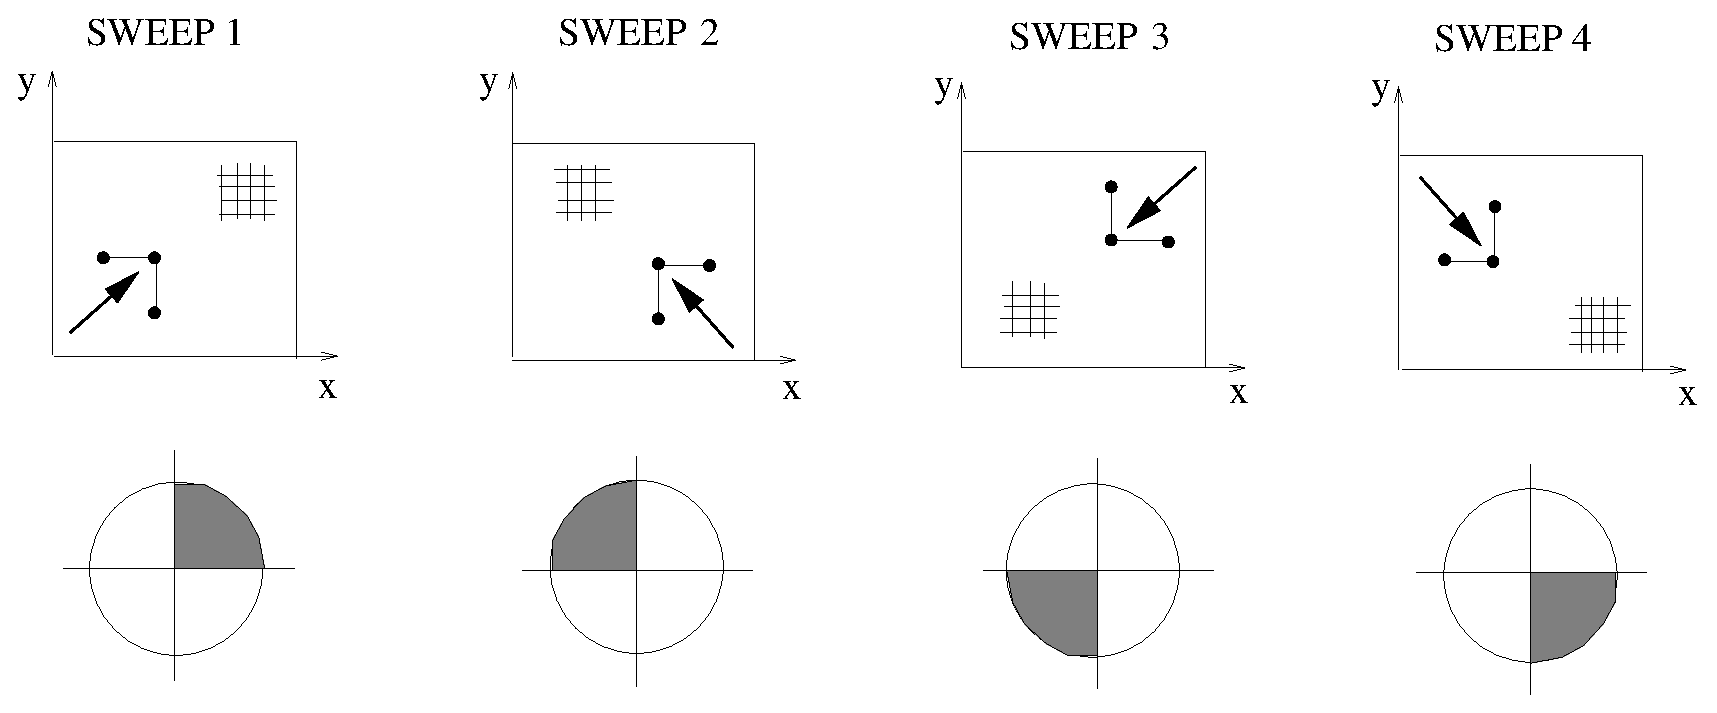
\epsfig{file=4sweep.eps,height=6cm}
              }
      \caption{The solution procedure for wave energy propagation in geographical space with the appropriate
               directional quadrant (indicated by shaded area) for each of four sweeps.}
      \label{fig:4sweep}
\end{figure}
propagation terms in (\ref{eq:actdisc}), a system of equations must
be formed.
Furthermore, due to the fact that the source term $S_{\rm tot}$ in (\ref{eq:actdisc}) is nonlinear in $N$,
linearization
is required in order to find a solution. Generally, the term $S_{\rm tot}$ in each bin $(l,m)$ is treated by
distinguishing between positive and negative contributions and arranging these in the linear form
(Ferziger and Peri\'{c}, 1999):
\begin{equation}
  S_{\rm tot} = S_{\rm tot}^p + S_{\rm tot}^n N \, ,
  \label{eq:srcpn}
\end{equation}
where $S_{\rm tot}^p$ consists of positive contributions and
$S_{\rm tot}^n$ of negative ones. Both contributions are independent of the solution $N$ at the corresponding bin $(l,m)$.
Any negative term that does not contain $N$ as a multiplier is first
divided by $N$ obtained from the previous iteration level and then added to $S_{\rm tot}^n$.
This stabilizes the iteration process.
Details on the application of this principle to each source term in SWAN can be found in Booij~{\it et~al}. (1999).
\\[2ex]
\noindent
The strongly nonlinear source term of depth-induced wave breaking is linearized by means of the Newton-Raphson iteration,
as follows:
\begin{equation}
  S^n \approx \phi^{n-1} E^{n} + \left( \frac{\partial S}{\partial E} \right)^{n-1} (E^n - E^{n-1})
\end{equation}
Since, this process of depth-induced wave breaking has been formulated such that $S = aS_{\rm tot}$ and $E = aE_{\rm tot}$,
the derivative $\partial S/\partial E$ is analytically determined as $\partial S_{\rm tot}/\partial E_{\rm tot}$. Here,
$a$ is identical in both expressions and the total energy $E_{\rm tot}$ and total source $S_{\rm tot}$ are the integrals
over all frequencies and directions of $E(\sigma,\theta)$ and $S_{\rm {ds,br}}(\sigma,\theta)$, respectively.
\\[2ex]
\noindent
As such, each difference equation (\ref{eq:actdisc}) using expressions (\ref{eq:fluxs}), (\ref{eq:fluxt})
and (\ref{eq:srcpn}) provides
an algebraic relation between $N$ at the corresponding bin and its nearest neighbours:
\begin{equation}
  a_{\rm P} N_{\rm P} = a_{\rm L} N_{\rm L}+
                                a_{\rm R} N_{\rm R}+
                                a_{\rm B} N_{\rm B}+
                                a_{\rm T} N_{\rm T}+
                                b_{\rm P} \, ,
  \label{eq:diffeq}
\end{equation}
where P corresponds to central bin $(l,m)$ and L(eft), R(ight), B(ottom)
and T(op) correspond to $(l-1,m)$, $(l+1,m)$, $(l,m-1)$ and $(l,m+1)$, respectively.
Furthermore, the coefficients
$a_k$, $k \in \{ \rm P,\rm L, \rm R, \rm B, \rm T \}$ arise from the
discretizations of the fluxes $c_{\sigma} N$ and $c_{\theta} N$ and $b_{\mathrm{P}}$ contains the positive contributions
of the source term $S_{\rm tot}^p$ in (\ref{eq:srcpn}) and the updated fluxes $c_x N$ (\ref{eq:fluxx}) and
$c_y N$ (\ref{eq:fluxy}). Note that coefficient $a_{\rm P}$ includes $-S_{\mathrm{tot}}^n$.
\\[2ex]
\noindent
The linear system of equations (\ref{eq:diffeq}) for all bins within a directional quadrant
at a particular geographical point is denoted by
\begin{equation}
  A \, \vec{N} = \vec{b} \, ,
  \label{eq:syseqs}
\end{equation}
where $A \in {\mbox{$I\!\!R$}}^{K \times K}$ contains the coefficients $a_k$, $k \in \{ \mathrm{P},
\mathrm{L}, \mathrm{R}, \mathrm{B}, \mathrm{T} \}$ (and
corresponds to a subblock on the main diagonal of (\ref{eq:matr})),
$\vec{b} \in {\mbox{$I\!\!R$}}^{K}$ contains the coefficient $b_{\rm P}$ and boundary values and
$\vec{N} \in {\mbox{$I\!\!R$}}^{K}$ denotes an algebraic vector containing the unknown
action density values. Matrix $A$ is non-symmetric. The dimension $K$ of a
directional quadrant equals $N_{\sigma} \times 1/4 N_{\theta}$.
Note that linearization of the source term (\ref{eq:srcpn}) enhances diagonal dominance of $A$, thereby improving numerical stability.
Also note that neither $A$ nor $\vec{b}$ depends on the unknowns.
Each row in the matrix $A$ corresponds to a bin
$(l,m)$. The main diagonal contains the coefficients
$a_{\rm P}$ and directly to the left and right are the coefficients
$-a_{\rm B}$ and $-a_{\mathrm{T}}$, respectively. The coefficients $-a_{\rm L}$ and $-a_{\rm R}$
are on the diagonals that are $N_{\theta}$ positions to the left and
right of the main diagonal, respectively.
\\[2ex]
\noindent
The solution $\vec{N}$ is given by $A^{-1} \vec{b}$. Since, the only non-zero matrix elements are situated in five diagonals,
iterative solution methods that utilize the sparsity of $A$ optimally are very attractive.
In SWAN,
the solution of (\ref{eq:syseqs}) is found by means of an incomplete lower-upper decomposition method followed by an
iteration process called the
Strongly Implicit Procedure (SIP) (Ferziger and Peri\'{c}, 1999). This procedure is specifically designed for
(non-symmetric) penta-diagonal systems and is relatively fast.
Note that in the absence of mean current there are no shifts
in the frequency, and consequently the structure of $A$ reduces to a tri-diagonal one, i.e.
$a_{\rm L} = a_{\rm R} = 0$, which can be inverted efficiently with
the Thomas algorithm (Press~{\it et~al}., 1993; Ferziger and Peri\'{c}, 1999).
\nocite{Fer99P}
\\[2ex]
\noindent
Due to refraction and nonlinear wave energy transfer, interactions occur
between the directional quadrants. To properly take these interactions into
account and the fact that we employ the Gauss-Seidel technique and linearization of the source term (\ref{eq:srcpn}),
the quadrant sweeping and the solution of system (\ref{eq:syseqs})
need to be repeated until some convergence criteria are met. At present,
the iteration process runs from $s = 1$ to $s = S$ and is terminated if the maximum number of
iterations $S$ (usually 15) is reached or the following criteria for the significant wave height $H_{m0}$ and mean
relative wave period $T_{m01}$, as given by
\begin{equation}
  H_{m0} = 4\sqrt{m_0}\, , \quad T_{m01} = 2\pi \frac{m_0}{m_1}\, , \quad
  m_j = \int_{0}^{\infty} \int_{0}^{2\pi} \sigma^j E(\sigma,\theta) d\sigma d\theta \, ,
\end{equation}
are both satisfied in at least 98\% of all wet grid points $(i,j)$:
\begin{equation}
  \frac{|\Delta H^{s}_{m0}(i,j)|}{H^{s-1}_{m0}(i,j)} <
  {\varepsilon}^{\rm r}_{\rm H} \quad \mbox{or} \quad
  |\Delta H^{s}_{m0}(i,j)| <
  {\varepsilon}^{\rm a}_{\rm H}
  \label{eq:stop}
\end{equation}
and
\begin{equation}
  \frac{|\Delta T^{s}_{m01}(i,j)|}{T^{s-1}_{m01}(i,j)} <
  {\varepsilon}^{\mathrm{r}}_{\mathrm{T}} \quad \mbox{or} \quad
  |\Delta T^{s}_{m01}(i,j)| <
  {\varepsilon}^{\rm a}_{\rm T} \, .
  \label{eq:stop2}
\end{equation}
Here, $\Delta Q^s \equiv Q^s - Q^{s-1}$, with $Q$ some quantity.
The default values of the limiting criteria are:
${\varepsilon}^{\rm r}_{\rm H} = {\varepsilon}^{\rm r}_{\rm T} = 0.02$,
${\varepsilon}^{\rm a}_{\rm H} = 0.02$ m and ${\varepsilon}^{\rm a}_{\rm T} = 0.2$ s.
The rationale behind the use of the integral wave parameters
$H_{m0}$ and $T_{m01}$ in the stopping criteria is that these are the output variables typically of interest.
The iterative solution procedure is accelerated by calculating a
reasonable first guess of the wave field based on second-generation source
terms of Holthuijsen and De Boer (1988).
\nocite{Hol88B}

\section{An illustrative explanation of the sweeping approach}
\label{sec:simple}

In the absence of a current, the direction of propagation of the wave crest is equal to that of the wave
energy. For this case, the propagation velocity of energy ($c_x$, $c_y$) is equal
to the group velocity ($c_{g,x}$, $c_{g,y}$). In presence of a current this is not the case, since the propagation
velocities $c_x$ and $c_y$ of energy are changed by the current. Considering the applied numerical procedure
in SWAN, it is initially more convenient to explain the basic principles of the numerical procedure in
the absence of a current than in the situation where a current is present. So, first, we shall focus on
the sweeping technique in the absence of a current. After this, we shall discuss the numerical
procedure in case a current is present.
\\[2ex]
\noindent
The computational region is a rectangle covered with a rectangular grid. One of the axes (say
the $x-$axis) is chosen arbitrary, for instance perpendicular to the coast.
The state in a grid point ($x_i$,$y_j$) in an upwind stencil is determined by its up-wave grid points
($x_{i-1}$,$y_j$) and ($x_i$,$y_{j-1}$). This stencil covers
the propagation of action density within a sector of 0$^o -$90$^o$, in the entire geographic space; see Figure~\ref{fig:fsweep}.
\begin{figure}[htb]
   \centerline{
      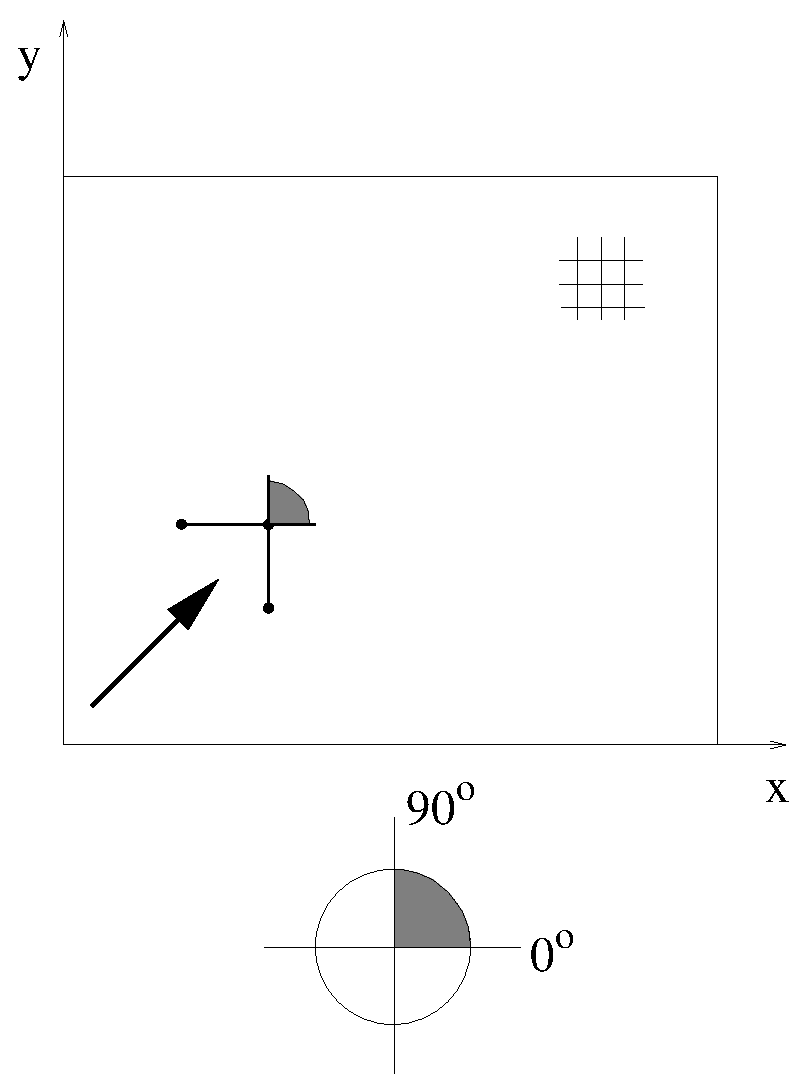
\epsfig{file=fsweep.eps,height=10cm}
              }
      \caption{Numerical scheme for wave propagation in geographic space with below the first quadrant for which the waves are propagated.}
      \label{fig:fsweep}
\end{figure}
Hence, this procedure is called
sweep 1 and encloses all wave energy propagation over the first quadrant. By rotating the stencil over
90$^o$, the next quadrant 90$^o -$180$^o$ is propagated. Rotating the stencil twice more ensures propagation over
all four quadrants (see Figure~\ref{fig:4sweep}). This allows waves to propagate from all directions. Hence, the method
is characterized as a four-sweep technique.
\\[2ex]
\noindent
The gain of such a stencil is that the propagation is unconditionally stable because the wave
characteristics lie within the concerning quadrant. Propagation is not subjected to a CFL criterion.
In cases with current refraction or bottom refraction, action density can shift from one quadrant to
another. This is taken into account in the model by repeating the computations with converging results
(iterative four-sweep technique). Typically, we choose a change of less then 1\% or so in significant wave
height and mean wave period in all geographic grid points to terminate the iteration (see Section~\ref{sec:sol}).
\\[2ex]
\noindent
The numerical procedure as described above remains in principle the same when a current ($U_x$,$U_y$) is present. The
main difference is that the propagation velocities of energy are no longer equal to the group velocity
of the waves but become equal to $c_x = c_{g,x}+U_x$ and $c_y = c_{g,y}+U_y$. To ensure an unconditionally
stable propagation of action in geographical space in the presence of any current, it is first determined
which spectral wave components of the spectrum can be propagated in one sweep. This implies that all wave
components with $c_x>0$ and $c_y>0$ are propagated in the first sweep, components with $c_x<0$ and $c_y>0$
in the second sweep, components with $c_x<0$ and $c_y<0$ in the third sweep, and finally, components $c_x>0$
and $c_y<0$ in the fourth sweep.
Since the group velocity of the waves decreases with increasing frequency, the higher frequencies
are more influenced by the current. As a result, the sector boundaries in directional space for these
higher frequencies change more compared to the sector boundaries for the lower frequencies. In general,
four possible configurations do occur (see Figure~\ref{fig:sweepcur}). Consider, for instance, one fixed frequency
propagating on a uniform current. The current propagates at an angle of 45$^o$ with the $x-$axis. The sign
of the current vector and strength of the current are arbitrary. The shaded sectors in Figure~\ref{fig:sweepcur}
indicate that all the wave components that are propagating in the direction within the shaded sector, are
propagated in the first sweep ($c_x>0$, $c_y>0$).
\begin{figure}[htb]
   \centerline{
      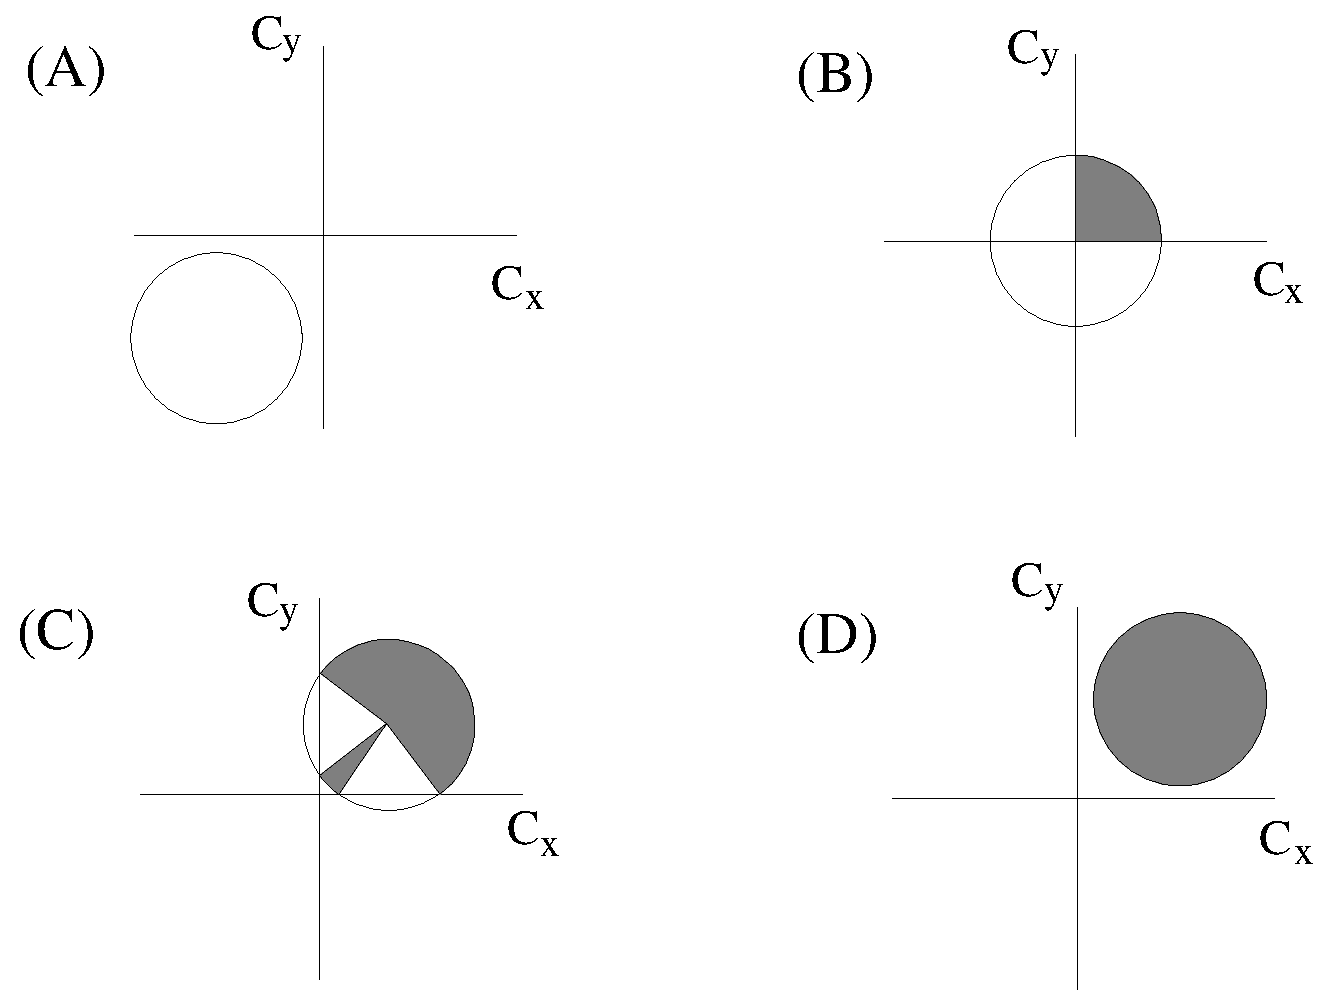
\epsfig{file=sweepcur.eps,height=10cm}
              }
      \caption{Four possible configurations and propagation velocities $c_x$, $c_y$ for a fixed frequency in the presence of
               a current propagating at an angle of 45$^o$ with the $x-$axis.}
      \label{fig:sweepcur}
\end{figure}
\\[2ex]
\noindent
The top-left panel (A) represents a situation in which both $c_x$ and $c_y$ are negative due to a strong
opposing current, i.e. wave blocking occurs. None of the wave components is propagated within the first
sweep. The top-right panel (B) represents a situation in which the current velocity is rather small.
The sector boundaries in directional space are hardly changed by the current such that the sector
boundaries are approximately the same as in the absence of a current. The bottom-left panel (C)
reflects a following current that causes the propagation velocities of the wave components in two
sectors to be larger than zero. In this specific case, all the waves of the shaded sectors are propagated
within the first sweep. The bottom-right panel (D) represents a case with a strong following current
for which all the action is take along with the current. For this case the fully 360$^o$ sector is
propagated in the first sweep.
\\[2ex]
\noindent
After it has been determined which wave components are propagated in one
sweep, i.e., the sector boundaries in directional space have been determined for each frequency, the
integration in frequency and directional space can be carried out for those wave components.

\section{Implementation of DIA within the four-sweep technique}

In SWAN, the quadruplets are integrated using the DIA, see Section~\ref{sec:quad}. As a
consequence of the four-sweep technique, two different types of methods can be used to calculate the
four wave-wave interactions.
\begin{enumerate}
\item
The first method implies that the interactions are calculated in every
iteration prior to the first sweep. This method ensures conservation of energy density, but has the
disadvantage that the spectral source term $S_{\rm nl4}(\sigma,\theta)$ for every grid point in
geographical space has to be stored in internal memory. Such an integration method increases the
amount of required memory with a factor about 2.
The source term is stored in memory and is then explicitly integrated for a particular sweep.
\item
The second method is slightly different, in which the interactions are
calculated and integrated for every sweep separately. The calculation of the energy transfer for a specific
quadrant requires also the calculation of the transfer within a sector of about 33$^o$ in the adjacent two
quadrants. Calculating the interactions for one sweep increases the
computation time for the quadruplets with a factor of about 1.66 (2 adjacent sectors of 33$^o$ times
4 sweeps divided by 360$^o$). Contrary to the first method, the total rate of this energy shift is
not stored in memory such that energy density is not conserved per sweep (and per iteration). However,
this does not influence the converging results.
Within this second method, two different numerical schemes are available, namely, a semi-implicit scheme
and a fully explicit scheme. The use of a fully explicit scheme is recommended because of the computational
efficiency. A semi-implicit scheme increases the computation time of the quadruplets with a factor of about 2.
\end{enumerate}

\section{Convergence-enhancing measures} \label{sec:stab}

As explained in Section~\ref{sec:intnum},
many time scales are involved in the evolution of wind waves. The high-frequency waves have much shorter
time scales than the low-frequency waves, rendering the system of equations
(\ref{eq:syseqs}) stiff. If no special measures are taken,
the need to resolve high-frequency waves at very short time scales would result in extreme computational time. For economy,
it is desirable that a numerical technique can be used with a large, fixed time step. Moreover, we are
mainly interested in the evolution of slowly changing low-frequency waves. For stationary problems,
we are interested in obtaining the steady-state solution.
Unfortunately, the convergence to the steady state is dominated by the
smallest time scale and, in the absence of remedial measures, destabilizing
over- and undershoots will prevent
solution from converging monotonically during the iteration process.
These oscillations arise because of the off-diagonal terms in matrix $A$,
which can be dominant over the main diagonal, particularly when the ratio
$\sigma_{\rm max}/\sigma_{\rm min}$ is substantially larger than one. As a consequence,
convergence is slowed down and divergence often occurs.
To accelerate the iteration process without generating instabilities, appropriately small updates must be made
to the level of action density.
\\[2ex]
\noindent
With the development of the WAM model, a so-called action density limiter was introduced as a remedy to the abovementioned
problem. This action limiter restricts the net growth or
decay of action density to a maximum change at each geographic grid point and spectral bin per time step.
This maximum change corresponds to a fraction of the
omni-directional Phillips equilibrium level (Hersbach and Janssen, 1999).
In the context of SWAN (Booij~{\it et~al}., 1999), this is
\begin{equation}
  \Delta N \equiv \gamma \, \frac{\alpha_{\rm PM}}{2 \sigma k^3 c_g} \, ,
  \label{eq:limit}
\end{equation}
where $\gamma \geq 0$ denotes the limitation factor, $k$ is the wave number and
$\alpha_{\rm PM} = 8.1 \times 10^{-3}$ is the Phillips constant for a Pierson-Moskowitz spectrum
(Komen~{\it et~al}., 1994). Usually, $\gamma = 0.1$ (Tolman,
1992)\footnote{It is
  noted here that the effective $\gamma$ used in SWAN is not equivalent to that of
   WAM: the former is a factor $2\pi$ larger.}.
Note that when the physical wind formulation of Janssen (1989,1991a) is applied in SWAN, the original
limiter of Hersbach and Janssen (1999) is employed. Denoting the
total change in $N_{i,j,l,m}$ from one iteration to the next after (\ref{eq:actdisc}) by
$\Delta N_{i,j,l,m}$, the action density at the new iteration level is given by
\begin{equation}
  N_{i,j,l,m}^s = N_{i,j,l,m}^{s-1} + \frac{\Delta N_{i,j,l,m}}{|\Delta N_{i,j,l,m}|} \,
  \min \{ | \Delta N_{i,j,l,m} |, \Delta N \} \, .
  \label{eq:updat}
\end{equation}
For wave components at relatively low frequencies, (\ref{eq:updat}) yields
the pre-limitation outcome of (\ref{eq:actdisc}), because, for these
components, the pseudo time step matches the time scale of their evolution. For
high-frequency waves, however, (\ref{eq:updat}) gives the upper limit for the
spectrum to change per iteration due to the limiter (\ref{eq:limit}).
For typical coastal engineering applications, it is sufficient to
compute the energy-containing part of the wave spectrum accurately.
In other words, action densities near and below the spectral peak should not be imposed
by the limiter (\ref{eq:limit}). However, our experiences with
SWAN have shown that the limiter is active even close to the peak. Furthermore,
during the entire iteration process, the limiter is typically active at
almost every geographic grid point.
\nocite{Her99J,Boo99RH,Kom94CDHHJ,Tol92a}
\\[2ex]
\noindent
The alternative measure to enhance the convergence of the stable iteration process considered here
is so-called false time stepping (Ferziger and Peri\'{c}, 1999).
Under-relaxation terms representing the rate of change are introduced to enhance the main
diagonal of $A$ and thus stabilize the iteration process. The system of equations
(\ref{eq:syseqs}) is replaced by the following, iteration-dependent system
\begin{equation}
  \frac{{\vec{N}}^s - {\vec{N}}^{s-1}}{\tau} + A\,{\vec{N}}^s = \vec{b}
  \label{eq:relax1}
\end{equation}
with $\tau$ a pseudo time step.
The first term of (\ref{eq:relax1}) controls the rate of
convergence of the iteration process in the sense that
smaller updates are made due to decreasing $\tau$, usually
at the cost of increased computational time.
To deal with decreasing time scales at
increasing wave frequency, the amount of under-relaxation is enlarged in
proportion to frequency. This allows a decrease in the computational cost of
under-relaxation, because at lower frequencies larger updates are made. This
frequency-dependent under-relaxation can be achieved by setting ${\tau}^{-1} = \alpha \sigma$,
where $\alpha$ is a dimensionless parameter.
The parameter $\alpha$ will play an important role in
determining the convergence rate and stability of the iteration process.
Substitution in (\ref{eq:relax1}) gives
\begin{equation}
  (A + \alpha \sigma I)\, {\vec{N}}^s = \vec{b} + \alpha \sigma {\vec{N}}^{s-1} \, .
  \label{eq:relax}
\end{equation}
When the steady state is
reached (i.e. $s \rightarrow \infty$), system (\ref{eq:relax}) solves $A\,{\vec{N}}^{\infty} = \vec{b}$ since,
${\vec{N}}^{\infty}$ is a fixed point of (\ref{eq:relax}).
\\[2ex]
\noindent
Suitable values for $\alpha$ must be determined empirically and thus robustness is impaired.
For increasing values of $\alpha$, the change in action density per iteration will decrease in
the whole spectrum. The consequence of this is twofold. Firstly, it allows a much broader frequency
range in which the action balance equation (\ref{eq:actdisc}) is actually solved without distorting convergence
properties.
Secondly, the use of the limiter will be reduced because more density changes will not exceed the maximum
change (\ref{eq:limit}). Clearly, this effect may be augmented by
increasing the value of $\gamma$ in (\ref{eq:limit}).
\\[2ex]
\noindent
To allow proper calculation of the second-generation first guess of the wave
field (see Section \ref{sec:sol}), under-relaxation is temporarily disabled
($\alpha = 0$) during the first iteration. Whereas this measure is important
in achieving fast convergence, it does not affect stability, since the
second-generation formulations do not require stabilization.

\section{Stopping criteria} \label{sec:stop}

In general, the iterative method should be stopped if the approximate solution is
accurate enough. A good termination criterion is very important, because if the criterion
is too weak the solution obtained may be useless, whereas if the criterion is too
severe the iteration process may never stop or may cost too much work.
Experiences with SWAN have shown that the present criteria (\ref{eq:stop}) and (\ref{eq:stop2}) are
often not strict enough to obtain accurate results after termination of the iterative
procedure.
Thus, criteria (\ref{eq:stop}) and (\ref{eq:stop2})
are necessary but not sufficient.
It was found that the iteration process can converge so slowly that at a certain
iteration $s$ the difference between the successive iterates, $H^s_{m0} - H^{s-1}_{m0}$,
can be small enough to meet the convergence criteria, causing the iteration process to stop, even though
the converged solution has not yet been found. In particular, this happens when convergence is non-monotonic
such that the process is terminated at local maxima or minima that may not coincide with the
converged solution.
\\[2ex]
\noindent
Furthermore, it became apparent
that, unlike $H_{m0}$, the quantity $T_{m01}$ is not an effective measure of
convergence. It was found that the relative error in $T_{m01}$, i.e.
$|T^s_{m01} - T^{s-1}_{m01}|/T^{s-1}_{m01}$, does not monotonically
decrease near convergence, but keeps
oscillating during the iteration process. This behaviour is due to small variations
in the spectrum at high frequencies, to which $T_{m01}$ is sensitive.
This
behaviour is problematic when any form of stricter stopping criterion is developed
based on $T_{m01}$. Therefore, in the improved termination criterion
proposed, $T_{m01}$ has been abandoned as a convergence
measure and only $H_{m0}$, which displays more monotonic behaviour near
convergence, is retained.
\\[2ex]
\noindent
Stiffness and nonlinearity of the action balance equation are found to yield less rapid and
less monotone convergence. Ferziger and Peri\'{c} (1999) explain the slow convergence
in terms of the eigenvalue or spectral radius of the iteration process generating the sequence
$\{{\phi}^0, {\phi}^1, {\phi}^2,...\}$. They show that the actual solution error
is given by
\begin{equation}
  {\phi}^{\infty} - {\phi}^s \approx \frac{{\phi}^{s+1} - {\phi}^s}{1-\rho} \, ,
\end{equation}
where ${\phi}^{\infty}$ denotes the steady-state solution and $\rho$ is the spectral radius
indicating the rate of convergence. The smaller $\rho$, the faster convergence. This result
shows that the solution error is larger than the difference between successive iterates.
Furthermore, the closer $\rho$ is to 1, the larger the ratio of solution error to the difference
between successive iterates. In other words, the lower the rate of convergence of the
iteration process, the smaller this difference
from one iteration to the next must be to guarantee convergence.
The stopping criterion of SWAN could be improved by making the maximum allowable relative increment
in $H_{m0}$ a function of its spectral
radius instead of imposing a fixed allowable
increment. By decreasing the allowable relative increment as
convergence is neared, it would be possible to delay run termination
until a more advanced stage of convergence.
Such a stopping criterion was used by, e.g. Zijlema and Wesseling (1998).
This criterion is adequate
if the iteration process converges in a well-behaved manner and $\rho < 1$ for all iterations.
However, due to nonlinearities SWAN typically does not display such
smooth behaviour. Therefore, this criterion may be less suited for SWAN.
\nocite{Zij98W}
\\[2ex]
\noindent
An alternative way to evaluate the level of convergence is to consider
the second
derivative or curvature of the curve traced by the series of iterates
(iteration curve). Since the curvature of the iteration curve must tend
towards zero as convergence is reached, terminating the
iteration process when a
certain minimum curvature has been reached would be a robust break-off procedure.
The curvature of the iteration curve of $H_{m0}$ may be expressed in the discrete sense as
\begin{equation}
  \Delta (\Delta \tilde{H}_{m0}^s)^s = \tilde{H}_{m0}^s - 2\tilde{H}_{m0}^{s-1} + \tilde{H}_{m0}^{s-2} \, ,
\end{equation}
where $\tilde{H}_{m0}^s$ is some measure of the significant wave height at
iteration level~$s$. To eliminate the effect of small amplitude
oscillations on the curvature measure, we define $\tilde{H}_{m0}^s
\equiv (H_{m0}^s +
H_{m0}^{s-1})/2$. The resulting curvature-based termination criterion at grid point $(i,j)$ is then
\begin{equation}
  \frac{| H_{m0}^s(i,j) - ( H_{m0}^{s-1}(i,j) + H_{m0}^{s-2}(i,j) ) +
  H_{m0}^{s-3}(i,j) | }{2 H_{m0}^s(i,j)}< \varepsilon_{\rm C} \, , \,\,\, s = 3, 4, ... \, ,
  \label{eq:stop3}
\end{equation}
where $\varepsilon_{\rm C}$ is a given maximum allowable curvature.
The curvature measure is made non-dimensional through normalization with $H_{m0}^s$.
Condition
(\ref{eq:stop3}) must be satisfied in at least 98\% of all wet grid points before the iterative process stops.
This curvature requirement is considered to be the primary criterion.
However, the curvature passes through zero between local maxima and minima and, at convergence, the solution
may oscillate between two constant levels due to the action limiter, whereas the average curvature is zero.
As safeguard
against such a situation, the weaker criterion (\ref{eq:stop}) is retained
in addition to the stricter criterion (\ref{eq:stop3}).

\section{Governing equations in curvi-linear co-ordinates} \label{sec:curvi}

A curvi-linear grid is characterized by the co-ordinates of the grid points, i.e.
\begin{equation}
  x_{i,j}\, , \qquad i=1,...,M \, , j=1,...,N
\end{equation}
\begin{equation}
  y_{i,j}\, , \qquad i=1,...,M \, , j=1,...,N
\end{equation}
The 4-sweep method is unchanged, so in the first sweep action densities in the points $(i-1,j)$ and $(i,j-1)$ are used to compute the action densities
in the point $(i,j)$. Numerical approximations are obtained by a 2-dimensional Taylor expansion with respect to the point $(x_{i,j},y_{i,j})$.
\\[2ex]
The differences in quantities between neighbouring grid points in the curvi-linear grid are denoted as follows:
\begin{equation}
  \Delta x_1 = x_{i,j} - x_{i-1,j} \, , \qquad \Delta y_1 = y_{i,j} - y_{i-1,j}\, , \qquad \Delta F_1 = F_{i,j} - F_{i-1,j}
\end{equation}
and
\begin{equation}
  \Delta x_2 = x_{i,j} - x_{i,j-1} \, , \qquad \Delta y_2 = y_{i,j} - y_{i,j-1}\, , \qquad \Delta F_2 = F_{i,j} - F_{i,j-1}
\end{equation}
The partial derivatives can be found from the 2-dimensional Taylor expansions:
\begin{equation}
  \Delta F_1 = \frac{\partial F}{\partial x} \Delta x_1 + \frac{\partial F}{\partial y} \Delta y_1
\end{equation}
and
\begin{equation}
  \Delta F_2 = \frac{\partial F}{\partial x} \Delta x_2 + \frac{\partial F}{\partial y} \Delta y_2
\end{equation}
It follows that the partial derivatives can be approximated by
\begin{equation}
  \frac{\partial F}{\partial x} \approx \frac{\Delta y_2 \Delta F_1 - \Delta y_1 \Delta F_2}{[D]}
\end{equation}
and
\begin{equation}
  \frac{\partial F}{\partial y} \approx \frac{\Delta x_1 \Delta F_2 - \Delta x_2 \Delta F_1}{[D]}
\end{equation}
where
\begin{equation}
  [D] = \Delta y_2 \Delta x_1 - \Delta y_1 \Delta x_2
\end{equation}
Thus, in curvi-linear co-ordinates the complete propagation terms (including time-derivative, but ignoring dependence on $\sigma$ and $\theta$ temporarily) read:
\begin{eqnarray}
  && \left ( \frac{1}{\Delta t} + (D_{x,1} + D_{x,2})c_{x,i,j}^+ + (D_{y,1}+D_{y,2}) c_{y,i,j}^+ \right ) N_{i,j}^+ \nonumber \\
  && - \frac{N_{i,j}^-}{\Delta t} - D_{x,1} (c_x N)_{i-1,j}^+ - D_{y,1} (c_y N)_{i-1,j}^+ \nonumber \\
  && - D_{x,2} (c_x N)_{i,j-1}^+ - D_{y,2} (c_y N)_{i,j-1}^+ = S_{i,j}^+
\end{eqnarray}
where
\begin{equation}
  D_{x,1} = \frac{\Delta y_2}{[D]} \, , \quad
  D_{y,1} = -\frac{\Delta x_2}{[D]} \, , \quad
  D_{x,2} = -\frac{\Delta y_1}{[D]} \, , \quad
  D_{y,2} = \frac{\Delta x_1}{[D]}
\end{equation}
Here, the superscript $+$ denotes the new time level $t$, and $-$ the old time level $t-\Delta t$. The equation for a stationary computation is found
by putting $1/\Delta t$ to 0.
\\[2ex]
Again, the marching method is stable as long as the propagation direction towards the point $(i,j)$ is enclosed between the lines connecting this point
with its neighbours $(i-1,j)$ and $(i,j-1)$. It can be shown that this is the case if
\begin{equation}
  D_{x,1}c_x + D_{y,1}c_y \geq 0\, \quad \mbox{and} \quad D_{x,2}c_x + D_{y,2}c_y \geq 0
\end{equation}
This set of criterions enables the SWAN program to decide whether a certain spectral direction does belong in the sweep which is being processed (in
this the first sweep).
\\[2ex]
In the second sweep, $\Delta x_1 = x_{i,j} - x_{i,j-1}$, etc. and $\Delta x_2 = x_{i,j} - x_{i+1,j}$, etc. In the third sweep,
$\Delta x_1 = x_{i,j} - x_{i+1,j}$, etc. and $\Delta x_2 = x_{i,j} - x_{i,j+1}$, etc. In the fourth sweep,
$\Delta x_1 = x_{i,j} - x_{i,j+1}$, etc. and $\Delta x_2 = x_{i,j} - x_{i-1,j}$, etc. Otherwise, all of the above equations and conditions remain
the same.
\\[2ex]
Conservation of action in the numerical approximation can be demonstrated for the triangle of which the corners are the three points $(i,j)$, $(i-1,j)$ and $(i,j-1)$.
If for each side of this triangle the flux is computed as the outer product of the average $cN$ and the side itself, then the three fluxes are exactly in balance
assuming that the situation is stationary, and the source term is zero. In this case it is found that:
\begin{eqnarray}
  && \left [ c_x N \right ]_{i,j}^{+} (\Delta y_2 - \Delta y_1) + \left [ c_x N \right ]_{i-1,j}^{+} (-\Delta y_2) +
  \left [ c_x N \right ]_{i,j-1}^{+} (\Delta y_1) + \nonumber \\
  && \left [ c_y N \right ]_{i,j}^{+} (\Delta x_1 - \Delta x_2) + \left [ c_y N \right ]_{i-1,j}^{+} (\Delta x_2) +
  \left [ c_y N \right ]_{i,j-1}^{+} (-\Delta x_1) = 0
\end{eqnarray}

\section{Computation of force in curvi-linear co-ordinates}

{\tt FORCE} is the wave-driven stress, i.e. the force per unit surface driving the wave-driven current, expressed in N/m$^2$, is defined
as the derivative of the radiation stresses:
\begin{equation}
  S_{xx} = \rho g \int \lfloor n \cos^2\theta + n - \frac{1}{2} \rfloor E d\sigma d\theta
\end{equation}
\begin{equation}
  S_{xy} = S_{yx} = \rho g \int n \sin\theta \cos\theta E d\sigma d\theta
\end{equation}
\begin{equation}
  S_{yy} = \rho g \int \lfloor n \sin^2\theta + n - \frac{1}{2} \rfloor E d\sigma d\theta
\end{equation}
Here, $n$ is the ratio of group velocity and phase velocity, i.e.
\begin{equation}
  n = \frac{c_g k}{\omega}
\end{equation}
The force is then
\begin{equation}
  F_x = -\frac{\partial S_{xx}}{\partial x} - \frac{\partial S_{xy}}{\partial y}
\end{equation}
and
\begin{equation}
  F_y = -\frac{\partial S_{yx}}{\partial x} - \frac{\partial S_{yy}}{\partial y}
\end{equation}
\\[2ex]
\noindent
In order to compute the force, the derivative of the radiation stress tensor has to be taken.
Let $f$ be one of the components of the tensor. We have to derive expressions for $\partial f/\partial x$ and
$\partial f/\partial y$. Derivatives with respect to the computational grid co-ordinates $\xi$ and $\eta$
can easily be found. The transformation is based on:
\begin{equation}
  \frac{\partial f}{\partial \xi} = \frac{\partial f}{\partial x}\frac{\partial x}{\partial \xi} +
                                    \frac{\partial f}{\partial y}\frac{\partial y}{\partial \xi}
\end{equation}
and
\begin{equation}
  \frac{\partial f}{\partial \eta} = \frac{\partial f}{\partial x}\frac{\partial x}{\partial \eta} +
                                    \frac{\partial f}{\partial y}\frac{\partial y}{\partial \eta}
\end{equation}
Hence,
\begin{equation}
  \frac{\partial f}{\partial x} = \frac{\frac{\partial f}{\partial\xi}\frac{\partial y}{\partial\eta}-\frac{\partial f}{\partial\eta}\frac{\partial y}{\partial\xi}}
                                       {\frac{\partial x}{\partial\xi}\frac{\partial y}{\partial\eta}-\frac{\partial x}{\partial\eta}\frac{\partial y}{\partial\xi}} =
  \frac{\partial f}{\partial \xi}\frac{\partial \xi}{\partial x} + \frac{\partial f}{\partial \eta}\frac{\partial \eta}{\partial x}
\end{equation}
and
\begin{equation}
  \frac{\partial f}{\partial y} = \frac{\frac{\partial f}{\partial\xi}\frac{\partial x}{\partial\eta}-\frac{\partial f}{\partial\eta}\frac{\partial x}{\partial\xi}}
                                       {\frac{\partial y}{\partial\xi}\frac{\partial x}{\partial\eta}-\frac{\partial y}{\partial\eta}\frac{\partial x}{\partial\xi}} =
  \frac{\partial f}{\partial \xi}\frac{\partial \xi}{\partial y} + \frac{\partial f}{\partial \eta}\frac{\partial \eta}{\partial y}
\end{equation}
Numerical approximations are quite simple:
\begin{equation}
  \frac{\partial f}{\partial \xi} \approx \frac{f_{\xi+1,\eta} - f_{\xi-1,\eta}}{2}\, , \qquad
  \frac{\partial f}{\partial \eta} \approx \frac{f_{\xi,\eta+1} - f_{\xi,\eta-1}}{2}
\end{equation}
These expressions are also used for derivatives of $x$ and $y$. On the boundaries of the computational region a one-sided approximation can be used.

\section{Numerical treatment of obstacles}
\label{sec:numobst}

An obstacle is treated in SWAN as a line running through the computational grid, see Figure~\ref{fig:obsgrid}.
When treating one grid point SWAN will first determine whether one of the grid lines of the stencil
crosses an obstacle; see Section~\ref{sec:cross} for the procedure to determine whether or not there is a crossing point.
If there is a crossing it will fall back to the first order upwind scheme.
\begin{figure}[htb]
   \centerline{
      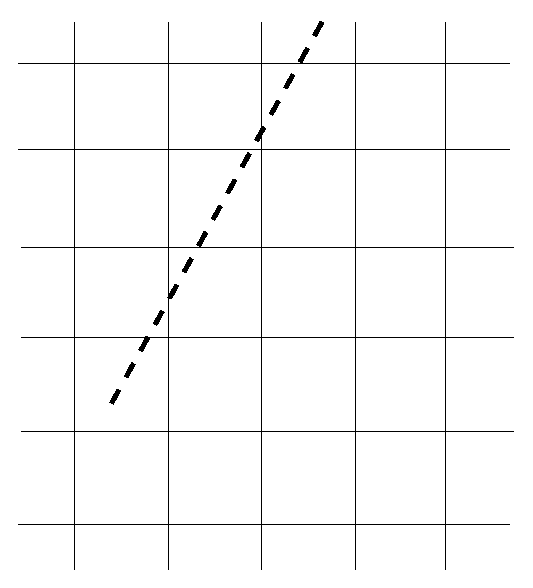
\epsfig{file=obsgrid.eps,height=5cm}
              }
      \caption{An obstacle as a line in computational grid.}
      \label{fig:obsgrid}
\end{figure}
\\[2ex]
\noindent
In computing the action densities for the target grid point (point 0 in Figure~\ref{fig:stencil1}),
\begin{figure}[htb]
   \centerline{
      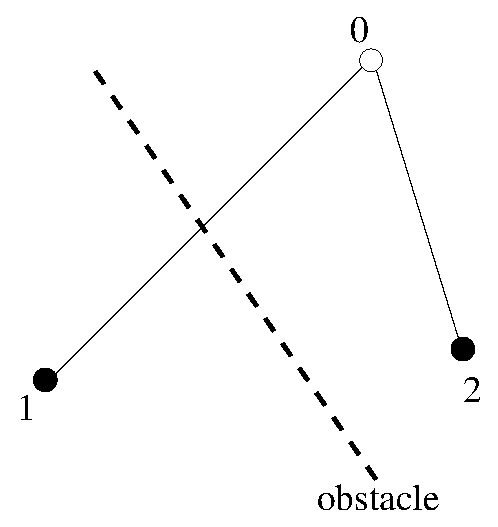
\epsfig{file=stencil1.eps,height=6cm}
              }
      \caption{Schematic sketch of transmission in SWAN.}
      \label{fig:stencil1}
\end{figure}
the contribution of a neighbouring grid point (point 1 in this case) is reduced by $K_t^2$,
if the connection between the two grid points crosses the obstacle.
(Note that the power 2 comes from the definition of the transmission coefficient which is
in terms of wave height).
The contribution from point 2 in the computation of point 0 is not reduced because there is no obstacle
crossing in between; the program takes $K_t=1$ for this point.
\\[2ex]
\noindent
A consequence of the above procedure is that the results are the same as long
as the obstacle crosses the same grid lines.
Thus the results for the situation shown would be the same
if the obstacle would be longer as long as the end would be in the same mesh.
Another consequence is that an obstacle has to cross at least
a few grid lines in order to have a noticeable effect, see Figure~\ref{fig:obsgrid}.
\\[2ex]
\noindent
After the transmission coefficient has been calculated, it is used in
the propagation terms of the action balance equation.
In curvi-linear coordinates, the propagation terms
(including time-derivative, but ignoring dependence on
$\sigma$ and $\theta$ temporarily) read:
\begin{eqnarray}
  && \left ( \frac{1}{\Delta t} + (D_{x,1} + D_{x,2})c_{x,i,j}^+ + (D_{y,1}+D_{y,2}) c_{y,i,j}^+ \right ) N_{i,j}^+ \nonumber \\
  && - \frac{N_{i,j}^-}{\Delta t} - D_{x,1} (c_x K^2_{t,1} N)_{i-1,j}^+ - D_{y,1} (c_y K^2_{t,1} N)_{i-1,j}^+ \nonumber \\
  && - D_{x,2} (c_x K^2_{t,2} N)_{i,j-1}^+ - D_{y,2} (c_y K^2_{t,2} N)_{i,j-1}^+ = S_{i,j}^+
\end{eqnarray}
In order to simplify the procedure, a reflected wave in a grid point is calculated
from the incident wave components in the same grid point.
This introduces numerical inaccuracies, but that is not uncommon in numerical models.
A basic condition in numerical models is that the approximation approaches the correct limit
as smaller and smaller step sizes are used.
\\[2ex]
\noindent
A reflected wave component in the target grid point 0, as illustrated by the arrow pointing
away from the obstacle in Figure~\ref{fig:stencil2},
\begin{figure}[htb]
   \centerline{
      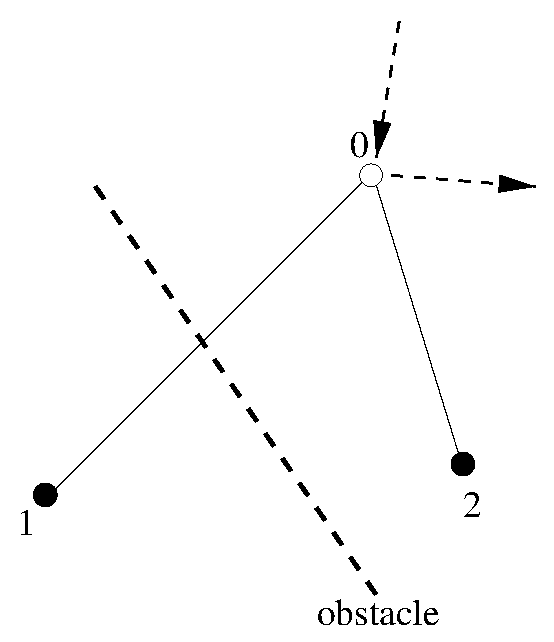
\epsfig{file=stencil2.eps,height=6cm}
              }
      \caption{Schematic sketch of reflection in SWAN.}
      \label{fig:stencil2}
\end{figure}
would get contributions from grid points 1 and 2 if there would not be an obstacle.
If the obstacle is there in the way shown, the contribution from point 2 is unchanged,
but the contribution from point 1 is
\begin{itemize}
  \item reduced by a transmission coefficient and
  \item partially replaced by the reflection of an incoming component in point 0.
\end{itemize}
Reflection only works when both grid points 0 and 1, as shown in Figure~\ref{fig:stencil2}, are wet points. This implies
that obstacle lines are only effective when bordered by wet points on both sides of the obstacle.

\section{Crossing of obstacle and grid line}
\label{sec:cross}

In the procedure for obstacles it is necessary to determine the crossing point of the obstacle and a grid line in the computational grid.
The obstacle is composed of straight sides. Let one side have the end points $\vec{x}_3 = (x_3,y_3)$ and $\vec{x}_4 = (x_4,y_4)$.
The end points of the grid line (both computational grid points) are
$\vec{x}_1=(x_1,y_1)$ and $\vec{x}_2 = (x_2,y_2)$. The crossing point must obey the following equation
\begin{equation}
  \vec{x}_1 + \lambda (\vec{x}_2-\vec{x}_1) = \vec{x}_3 + \mu(\vec{x}_4-\vec{x}_3)
\end{equation}
where both $\lambda$ and $\mu$ must be between 0 and 1. It follows that
\begin{equation}
  \lambda = \frac{(x_1-x_3)(y_2-y_1) - (y_1-y_3)(x_2-x_1)}
                 {(x_4-x_3)(y_2-y_1) - (y_4-y_3)(x_2-x_1)}
\end{equation}
and
\begin{equation}
  \mu = \frac{(x_1-x_3)(y_4-y_3) - (y_1-y_3)(x_4-x_3)}
             {(x_4-x_3)(y_2-y_1) - (y_4-y_3)(x_2-x_1)}
\end{equation}
If the denominator in both expressions is zero, the two lines are parallel and it is assumed that there is no crossing.

\section{Integration over $\sigma$}

Two methods are considered in SWAN for integration over frequency space. The first method is the common
trapezoidal rule. We consider the following integration
\begin{equation}
  I = \int_{0}^{\sigma_m} f\,E(\sigma)d\sigma
  \label{eq:pmomint}
\end{equation}
where $\sigma_m$ is the highest spectral frequency and $f$ is an arbitrary function. Usually, this function may be
$\sigma^p$, $\omega^p$ or $k^p$ with $p$ a power. We assume a discrete (logarithmic) distribution
of frequencies: $\sigma_{i}\, ,i=1,...,m$.
The approximation of (\ref{eq:pmomint}) is as follows:
\begin{equation}
  I \approx \sum_{2}^{m} \frac{1}{2}(f_{i-1} \sigma_{i-1} N_{i-1} + f_{i} \sigma_{i} N_{i})(\sigma_{i} - \sigma_{i-1})
\end{equation}
The contribution by the tail needs to be added as well, as follows. The tail of the energy density is proportional to $\sigma^{-P^*}$.
We have,
\begin{equation}
  \int_{\sigma_m}^{\infty} R \sigma^{-P^*} d\sigma = \sigma_{m} \frac{R \sigma_{m}^{-P^*}}{P^*-1}
\end{equation}
Assuming that a function $f$ has a tail with power $P^*$, so that $R \sigma_{m}^{-P^*} = f(\sigma_{m})$.
Hence,
\begin{equation}
  \int_{\sigma_m}^{\infty} f(\sigma)d\sigma = \frac{\sigma_{m}}{P^*-1} f(\sigma_{m})
\end{equation}
This integration is only valid if $P^* > 1$.
\\[2ex]
The second technique for integration over $\sigma$ makes use of the logarithmic discrete distribution of frequencies.
We introduced two variables in SWAN: {\tt FRINTF} and {\tt FRINTH}. The first is equal to
$\ln(\sigma_{i+1}/\sigma_{i})$, the latter to $\sqrt{\sigma_{i+1}/\sigma_{i}}$. Hence,
$\sigma_i = e^{\mu i}$ with $\mu = \ln(\sigma_{i+1}/\sigma_{i})$ and can be approximated as
$\mu = \Delta \sigma/\sigma$.
\\[2ex]
The integral over a function of $\sigma$, i.e. $f(\sigma)$ is transformed as follows:
\begin{equation}
  \int f(\sigma) d\sigma = \int f(\sigma) \mu e^{\mu i} di = \mu \int f(\sigma)\sigma di
\end{equation}
Thus, the integral can be approximated as
\begin{equation}
  \int f(\sigma)d\sigma \approx \mu \sum f_i \sigma_i
\end{equation}
The boundaries of a mesh in $\sigma-$space are $\sigma_i/\sqrt{\sigma_{i+1}/\sigma_{i}}$
and $\sigma_i \sqrt{\sigma_{i+1}/\sigma_{i}}$.
\\[2ex]
Computation of the contribution by the tail is done as follows. It is assumed that in the tail
the energy density is proportional to $\sigma^{-P^*}$. Furthermore, the discrete integration extends
to $M\cdot\sigma_m$, where
$M = \sqrt{1+\Delta \sigma/\sigma}$. Then the contribution by the tail is:
\begin{equation}
  \int_{\theta=0}^{2\pi} \int_{M\sigma_m}^{\infty} R \sigma^{-P^*} d\sigma d\theta =
  R \frac{M^{1-P^*} \cdot \sigma^{1-P^*}_{m}}{P^* - 1} =
  \frac{\sigma_m}{(P^*-1)M^{P^*-1}} R \sigma^{-P^*}_{m}
\end{equation}
Assuming that a function $f$ has a tail with power $P^*$, the integral over $f$ has a tail contribution of
\begin{equation}
  \int_{\theta=0}^{2\pi} \int_{M\sigma_m}^{\infty} f(\sigma)d\sigma d\theta =
  \frac{\sigma_m}{(P^*-1)M^{P^*-1}} f(\sigma_m)
\end{equation}
Since, $M$ is close to 1, the tail factor can be approximated as
\begin{equation}
  \frac{\sigma_m}{(P^*-1)M^{P^*-1}} \approx \frac{\sigma_m}{(P^*-1)(1+(P^*-1)(M-1))}
\end{equation}
In the SWAN program, we have $M=${\tt FRINTH}, $P^*=${\tt PWTAIL(1)} and $m=${\tt MSC}. The value of $P^*$
depends on the quantity that is integrated. For instance, in the computation of $\overline{k}$,
$P^*=P-2n-1$. Note that it is required that $P^*>1$, otherwise the integration fails.

\section{Transformation from relative to absolute frequency}

Internally, SWAN use action density as function of direction and relative (angular) frequency. Users may want
to obtain results in terms of absolute frequency, if only because measurements were taken at fixed positions.
\\[2ex]
Two modifications of the SWAN model that were needed to supply the information to the users are
\begin{itemize}
  \item the computation of integrated quantities such as average absolute frequency and
  \item the transformation of action or energy density.
\end{itemize}
The average absolute frequency is determined as follows:
\begin{equation}
  \overline{\omega} = \frac{\int \omega E(\sigma,\theta)d\sigma d\theta}{\int E(\sigma,\theta)d\sigma d\theta}
\end{equation}
The transformation of action or energy density from relative frequency $\sigma$ to absolute frequency $\omega$
is complicated because the mapping is not one-to-one, and therefore the Jacobian can become infinite. The
value of $\omega$ is determined by $\omega = W(\sigma)$.
\\[2ex]
The transformation is designed such that the following requirements are met:
\begin{itemize}
  \item If current velocities tend to zero the action densities for absolute frequency become identical
        with the densities with respect to relative frequency.
  \item The total energy density with respect to relative density is identical with the total energy density
        with respect to absolute density.
\end{itemize}
Furthermore, it is assumed that the distribution of absolute frequencies is the same as the distribution of
relative frequencies.
\\[2ex]
In the continuous model the mapping is done by
\begin{equation}
  E(\omega.\theta) = \int E(\sigma,\theta)\delta (\omega-W(\sigma)) d\sigma
\end{equation}
This relation is discretized whereby the energy density is assumed to be constant over intervals from
$\sigma_i/M$ to $M\sigma_i$.

\section{Interpolation of spectra}

The interpolation of spectra in SWAN, both in space and time, is a slight modification of the procedure
as used in WAM. This procedure is not a simple (spectral) bin-by-bin interpolation because that would cause
reduction of the spectral peak if the peaks of the original spectra do not coincide. It is an interpolation
where the spectra are first normalized by average frequency and direction, then interpolated and then
transformed back.
\\[2ex]
The average frequencies of the two origin spectra are determined using the frequency moments of the
spectra
\begin{equation}
  m_{i,k} = \int N_{i} (\sigma,\theta)\sigma^k d\sigma d\theta
\end{equation}
with $i$=1,2 (the two origin
spectra) and $k$=0,1 (the zero- and first frequency moments of these spectra). Then
\begin{equation}
  \overline{\sigma}_{i} = \frac{m_{i,1}}{m_{i,0}}
\end{equation}
The average frequency for the interpolated spectrum
is calculated as
\begin{equation}
  \overline{\sigma} = (w_{1} m_{1,1} + w_{2} m_{2,1})/(w_{1} m_{1,0} + w_{2} m_{2,0})
\end{equation}
where $w_{1}$ is the relative distance (in space or time) from the interpolated spectrum to the first
origin spectrum $N_{1}(\sigma,\theta)$ and $w_{2}$ is the same for the second origin spectrum
$N_{2}(\sigma,\theta)$. Obviously, $w_{1} + w_{2} = 1$.
\\[2ex]
The average directions of the two origin spectra are determined using directional moments of the spectra:
\begin{equation}
  m_{i,x} = \int N_{i} (\sigma,\theta) \cos (\theta) d\sigma d\theta
\end{equation}
and
\begin{equation}
  m_{i,y} = \int N_{i} (\sigma,\theta) \sin (\theta) d\sigma d\theta
\end{equation}
with $i$=1,2. The average direction is then
\begin{equation}
  {\overline{\theta}}_{i} = \mbox{atan} (\frac{m_{i,y}}{m_{i,x}})
\end{equation}
The average direction of the interpolated spectrum is calculated as
\begin{equation}
  \overline{\theta} = \mbox{atan} [\frac{w_{1} m_{1,y} + w_{2} m_{2,y}}{w_{1} m_{1,x} + w_{2} m_{2,x}}]
\end{equation}
Finally the interpolated spectrum is calculated as follows:
\begin{equation}
  N(\sigma,\theta) = w_{1} N_{1} [\overline{\sigma}_{1} \sigma/\overline{\sigma}, \theta -
  (\overline{\theta} - {\overline{\theta}}_{1} ) ] + w_{2} N _{2} [{\overline{\sigma}}_{2} \sigma /
  \overline{\sigma}, \theta - (\overline{\theta}-{\overline{\theta}}_{2})]
\end{equation}

\section{Computation of breaking source term}

The surf breaking dissipation of Battjes and Janssen (1978) reads
\begin{equation}
  D_{\rm tot} = -\alpha_{\rm BJ} Q_{b} \tilde{\sigma} \frac{H^2_{\rm max}}{8\pi}
\end{equation}
The surf breaking source term for each spectral bin $i$ is
\begin{equation}
  S_{i} = \frac{D_{\rm tot}}{E_{\rm tot}} E_i = {\tilde D}\, E_i
  \label{eq:st1}
\end{equation}
with the normalized total dissipation
\begin{equation}
  {\tilde D} = -\frac{\alpha_{\rm BJ} \tilde{\sigma} Q_{b}}{\pi {\cal B}} < 0
\end{equation}
and
\begin{equation}
  {\cal B} = \frac{8E_{\rm tot}}{H^2_{\rm max}} = \left( \frac{H_{\rm rms}}{\gamma d} \right)^2
\end{equation}
Since, the source term is strongly nonlinear in $E$ (since ${\tilde D}$ depends on $E$ through ${\cal B}$), we apply the Newton linearisation
to approximate the source term at iteration level $n+1$, as follows:
\begin{equation}
   S^{n+1}_{i} \approx {\tilde D} E_i^{n} + \left( \frac{\partial S}{\partial E} \right)_i^n (E_i^{n+1} - E_i^n)
   \label{eq:newlin}
\end{equation}
In SWAN, this approximation has been slightly adapted for reasons of numerical stability; the first term in the right-hand
side, ${\tilde D} E_i^{n}$, is replaced by ${\tilde D} E_i^{n+1}$. This preserves positivity of energy density $E$, if the following
inequality holds
\begin{equation}
  \frac{\partial S}{\partial E} < 0
\end{equation}
We derive an expression for this derivative as follows. From (\ref{eq:st1}), we have
\begin{equation}
  \frac{\partial S}{\partial E} |_i = \frac{\partial {\tilde D}}{\partial E}|_i E_i + {\tilde D}
\end{equation}
The normalized dissipation ${\tilde D}$ is a function of ${\cal B}$ which is proportional to $E$, so
\begin{equation}
  \frac{\partial S}{\partial E} |_i = \frac{\partial {\tilde D}}{\partial {\cal B}}|_i {\cal B}_i + {\tilde D}
  \label{eq:st4}
\end{equation}
Since, $Q_b$ is a function of ${\cal B}$, we get (using the quotient rule)
\begin{equation}
  \frac{\partial S}{\partial E} |_i = -\frac{\alpha_{\rm BJ} \tilde{\sigma}}{\pi}\, \frac{\partial Q_b}{\partial {\cal B}}
  \label{eq:st2}
\end{equation}
Since,
\begin{equation}
  1- Q_b + {\cal B} \ln Q_b = 0
  \label{eq:breakfract}
\end{equation}
the derivative of $Q_b$ is found by differentiating this with respect to ${\cal B}$:
\begin{equation}
  -{Q'}_{b} + \ln Q_b + \frac{\cal B}{Q_b} {Q'}_{b} = 0
\end{equation}
Hence,
\begin{equation}
  {Q'}_{b} = \frac{\ln Q_b}{1 - {\cal B}/Q_b} = \frac{Q_b}{\cal B} \frac{Q_b - 1}{Q_b - {\cal B}}
\end{equation}
using Eq. (\ref{eq:breakfract}). Now, ${Q'}_{b} > 0$, because $0 < Q_b < 1$ and ${\cal B} > Q_b$.
Substitution in (\ref{eq:st2}) gives
\begin{equation}
  \frac{\partial S}{\partial E} |_i = {\tilde D} \, \frac{Q_b - 1}{Q_b - {\cal B}} |_i < 0
\end{equation}
Finally, the approximation of the source term reads
\begin{equation}
  S^{n+1}_{i} = {\tilde D} \left( 1 + \frac{Q_b - 1}{Q_b - {\cal B}} \right)_i^n E_i^{n+1} - {\tilde D} \, \frac{Q_b - 1}{Q_b - {\cal B}} |^n_i E_i^n
\end{equation}

\section{On the approximation of refraction on coarse grids in large-scale SWAN applications}

\subsection{Introduction}

In some large-scale applications SWAN is known to produce seemingly unstable results. One of the causes of the behaviour may be the fully implicit treatment of the refraction term.
In this treatment the value of $c_\theta$ is determined at the point where the action densities are to be updated. This is reasonable if its value does not vary too much over one
(spatial) step. This is true in most coastal applications.
\\[2ex]
In large scale applications, however, the depth may vary from one grid point to the next by a factor of 100 or more. Then the value of $c_\theta$ at the shallowest grid point is
not representative anymore of the interval between the two grid points, and it is justified to limit the value to one that is representative. The problem now is to find
a limitation which on the one hand guarantees smooth behaviour in large-scale applications and which has no influence on small-scale applications.

\subsection{The problem with refraction on coarse grids and how to deal with it}

We consider the following action balance equation
\begin{equation}
  \frac{\partial N}{\partial t} + \nabla_{\vec{x}} \cdot [({\vec{c}}_g + \vec{U}) N] +
  \frac{\partial c_\sigma N}{\partial \sigma} +
  \frac{\partial c_\theta N}{\partial \theta} = \frac{S_{\mathrm{tot}}}{\sigma}\, .
  \label{eq:actbal}
\end{equation}
This equation is discretized using the Method of Lines (MOL) in which the time integration is chosen independently from the space discretization. The propagation terms are approximated employing
higher order schemes in some forms of blending, i.e. upwind and central.
Time integration is based on the implicit Euler scheme while the source terms are linearized according to the well-known Patankar rules. However, the propagation
of action density in the geographic space is done in a carefully manner without solving a huge matrix, such that unconditional stability can be guaranteed.
This approach is based upon the four-direction Gauss-Seidel iteration technique. For details, see Booij et al. (1999) and Zijlema and Van der Westhuysen (2005).
\\[2ex]
It is interesting to note that the above described approach is equivalent to the application of the well-known semi-Lagrangian approximation\footnote{In fact, it is nothing more than the method of characteristics.}.
To this purpose we consider the material derivative of the action density
\begin{equation}
  \frac{dN}{dt} \equiv \frac{\partial N}{\partial t} + c_x \frac{\partial N}{\partial x} + c_y\frac{\partial N}{\partial y}
  \label{eq:matder}
\end{equation}
with $(c_x,c_y) = {\vec{c}}_g + \vec{U}$ the propagation velocity vector in the geographical space.
This material derivative indicates that the time rate of change is computed along the wave characteristics defined by the following ODEs
\begin{equation}
  \frac{dx}{dt} = c_x\, , \quad \frac{dy}{dt} = c_y\, .
\end{equation}
For the purpose of illustration the spatial derivatives are replaced by first order upwind differences.
If we assume $c_x$ and $c_y$ positive during the first sweep, see Figure~\ref{fig:fsweep2},
\begin{figure}[htb]
   \centerline{
      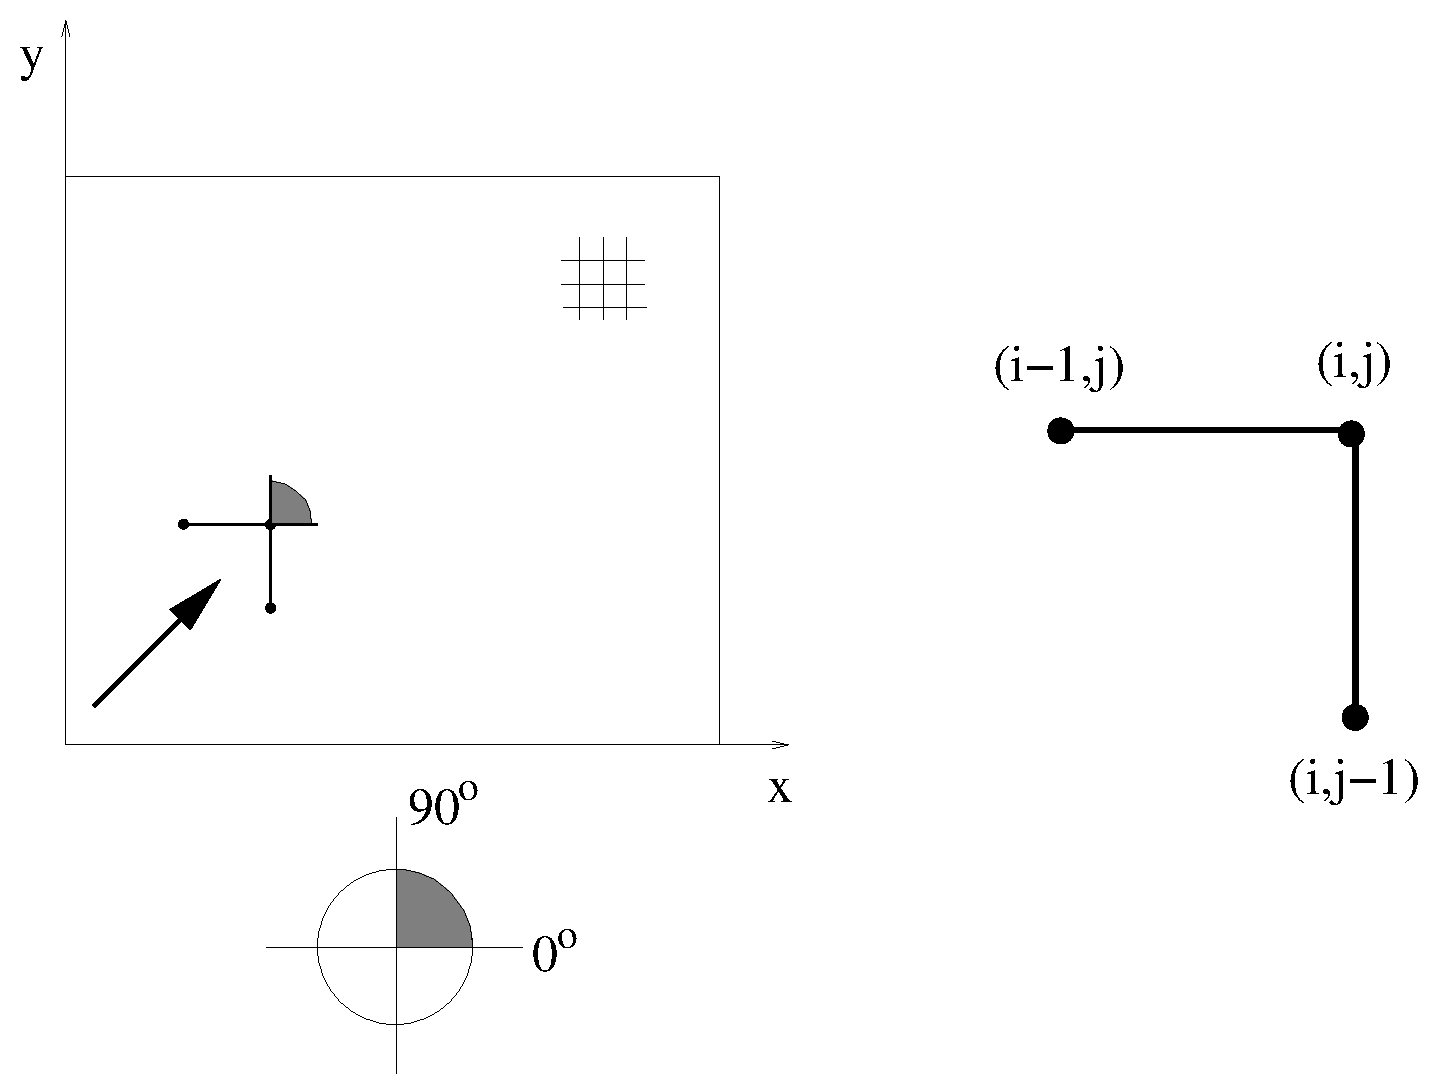
\epsfig{file=fsweep2.eps,height=8cm}
              }
      \caption{Numerical scheme for wave propagation in geographic space with below the first quadrant for which the waves are propagated, and right the stencil.}
      \label{fig:fsweep2}
\end{figure}
then the approximation of Eq. (\ref{eq:matder}) is as follows
\begin{equation}
 \frac{N^{n+1}_{i,j}-N^n_{i,j}}{\Delta t} + c_x \frac{N^{n+1}_{i,j} - N^{n+1}_{i-1,j}}{\Delta x} + c_y \frac{N^{n+1}_{i,j} - N^{n+1}_{i,j-1}}{\Delta y} \, .
\end{equation}
Note that the time integration is based on the first order implicit Euler scheme. Furthermore, $\Delta t$ is the time step, and $\Delta x$ and $\Delta y$ are the mesh spaces. This approximation can be rewritten as
\begin{equation}
  \left ( \frac{1}{\Delta t} + \frac{c_x}{\Delta x} + \frac{c_y}{\Delta y} \right )\, N^{n+1}_{i,j} - \frac{1}{\Delta t}N^{n+1}_{i,j} - \frac{c_x}{\Delta x} N^{n+1}_{i-1,j} - \frac{c_y}{\Delta y} N^{n+1}_{i,j-1}
\end{equation}
and this can be interpreted as an approximation of the material derivative, Eq. (\ref{eq:matder}), as follows
\begin{equation}
  \frac{N^{n+1}_{i,j} - N^{n}_{i^*,j^*}}{\Delta T}
\end{equation}
with
\begin{equation}
  \frac{1}{\Delta T} = \frac{1}{\Delta t} + \frac{c_x}{\Delta x} + \frac{c_y}{\Delta y}
\end{equation}
and
\begin{equation}
  i^* = i - p\, , \quad j^* = j - q\, , \quad p = \frac{c_x \Delta t}{\Delta x}\, , \quad q = \frac{c_y \Delta t}{\Delta y}\, .
\end{equation}
Note that $p$ and $q$ are the Courant numbers. They are not integers, and therefore $(i^*,j^*)$ is not a grid point. This point, however, lies on the wave characteristic. The quantity $N^{n}_{i^*,j^*}$ can be
interpreted as the value of $N$ at time $t^n$ in $(i^*,j^*)$ which is being convected in $(i,j)$ in a lapsed time $\Delta t$. This value is simply obtained from the interpolation of the surrounding values
$N^{n+1}_{i,j}$, $N^{n+1}_{i-1,j}$ and $N^{n+1}_{i,j-1}$ in the $(t,x,y)-$plane. In this case, there is no restriction on time step $\Delta t$ as the characteristic lies inside the computational stencil.
\\[2ex]
An important assumption made in this consideration is that $c_x$ and $c_y$ do not much vary over a time step. This is reasonable as the wave characteristics are more or less non-curved lines (during the time step), as
the propagation in the geographic space is slowly time varying. However, this is generally not the case for the spectral propagation. In particular, wave refraction due to bottom or current gradients is
typically a fast time-varying process. Often the associated time scale is much shorter than the desired time step used in a numerical simulation.
A consequence of this is that the energy can travel in one time or distance step over more than the length of one sweep (which in the absence of a current is 90$^o$,
see Figure~\ref{fig:fsweep2}). This is especially the case when the bathymetry is poorly resolved by the model as will be shown later.
Thus, for {\it physical} consistency, a restriction on the time step should be imposed in order for the wave direction not to cross the boundaries of a quadrant in the spectral space.
Specifically, the Courant number based on $\Delta T$ and $\Delta \theta$ (i.e. directional bin) should not exceed unity, that is,
\begin{equation}
  \mbox{Cr} \equiv \frac{|c_\theta| \Delta T}{\Delta \theta} \leq \alpha_\theta \leq 1
  \label{eq:courrefr}
\end{equation}
with $c_\theta$ the turning rate and $\alpha_\theta$ a user-defined maximum Courant number.
For example, consider the first sweep, see Figure~\ref{fig:fsweep2}, the boundaries of the first quadrant are the lines 0$^o$ and 90$^o$. Next, we consider the directional
sector in the spectral space associated with the considered sweep, see Figure~\ref{fig:sector}.
\begin{figure}[htb]
   \centerline{
      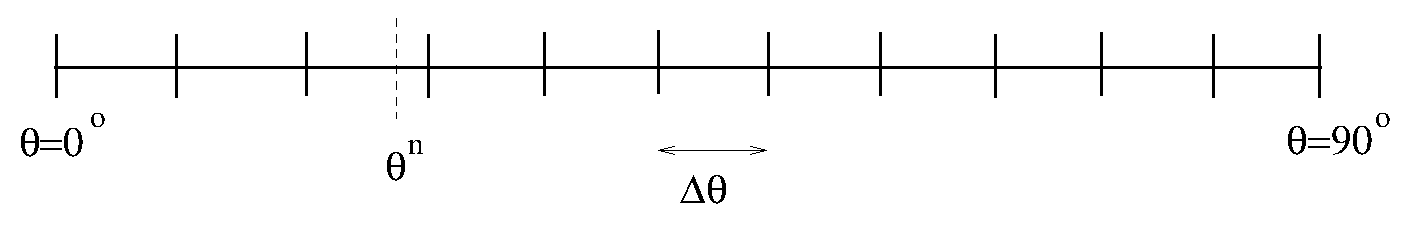
\epsfig{file=sector.eps,height=2cm}
              }
      \caption{Directional sector associated with the first sweep.}
      \label{fig:sector}
\end{figure}
We shall show that condition, Eq. (\ref{eq:courrefr}), is sufficient to assure that wave energy propagating in any bin in $\theta-$direction will not cross the boundaries of the directional sector,
except for the first and last bins. Since, by definition,
\begin{equation}
  \frac{d\theta}{dt} = c_\theta\, ,
\end{equation}
we may approximate this, as follows,
\begin{equation}
  \theta^{n+1} \approx \theta^n + c_\theta \Delta T\, .
  \label{eq:ctheta}
\end{equation}
For a given $n$, we choose an arbitrary point, $\theta^n$, inside the directional sector; see Figure~\ref{fig:sector}.
If $\theta^n \geq \Delta \theta$ then, Eqs. (\ref{eq:ctheta}) and (\ref{eq:courrefr}) imply
$|\theta^{n+1}-\theta^n| \leq \Delta \theta$, and hence the chosen point at next time step, $\theta^{n+1}$, still lies inside the directional sector. If $\theta^n < \Delta \theta$, i.e. in the first bin, then one obtains
\begin{equation}
  \theta^{n+1} = \theta^n + \frac{\Delta T}{\Delta \theta} \left[ (1-\theta^n) c_\theta(\theta=0^o) + \theta^n c_\theta(\theta=\Delta \theta) \right]
\end{equation}
or
\begin{equation}
  \theta^{n+1} = \theta^n \left ( 1 - \frac{\Delta T}{\Delta \theta} c_\theta(\theta=0^o) \right ) + \frac{\Delta T}{\Delta \theta} c_\theta(\theta=0^o) + \frac{\Delta T}{\Delta \theta}
  \theta^n c_\theta(\theta=\Delta \theta) \, .
\end{equation}
If $c_\theta(\theta=0^o) > 0$ and $c_\theta(\theta=\Delta \theta) > 0$ then, the point at next step will be keep inside the directional sector, if Eq. (\ref{eq:courrefr}) holds. In other cases the energy is leaving
through boundary $\theta = 0^o$, though the change in direction is limited to the adjacent directional bin of the other quadrant.
This holds also for the last bin and the corresponding right boundary $\theta = 90^o$.
\\[2ex]
Note that Eq. (\ref{eq:courrefr}) is {\em not required} for the stability of the method but contributes to improve its {\em physical} accuracy.
For instance, in a large-scale application, one often applies coarse (nested) grids with
a desired time step. Both the mesh width and the time step might be too large to represent wave refraction appropriately. This is readily seen as follows. We consider stationary, long-crested waves in $(x,\theta)-$space,
propagating at an angle with the positive $x-$axis. There are no currents. There is bottom gradient along this axis so that refraction is present. Hence, the Courant number becomes (cf. Eq. (\ref{eq:courrefr}))
\begin{equation}
  \mbox{Cr} = \frac{|c_\theta| \Delta x}{|c_g|\Delta \theta}
\end{equation}
with $c_g$ the group velocity. The turning rate is given by
\begin{equation}
  c_\theta = -\frac{1}{k} \frac{\partial \sigma}{\partial h}\frac{\partial h}{\partial m}\, ,
  \label{eq:ctheta1}
\end{equation}
where $k$ is the wave number, $\sigma$ is the frequency, $h$ is the water depth and $m$ is the coordinate along the wave crest (i.e. orthogonal to the propagation direction). On a coarse grid, both the mesh width
$\Delta x$ and the depth gradient $\partial h/\partial m$, and thereby $c_\theta$, can be very large. This implies that the CFL condition may be violated, i.e. $\mbox{Cr} > 1$.
\\[2ex]
Yet the value of $c_\theta$ in the shallowest grid point can be simply too large due to large bottom slopes over one mesh width so that wave energy will change direction over more than some directional bins
or even the directional sector.
To prevent this artefact a limitation on $c_\theta$ seems to be justified. Recalling Eq. (\ref{eq:courrefr}), a limitation would be
\begin{equation}
  |c_\theta| \leq \alpha_\theta \Delta \theta \left ( \frac{1}{\Delta t} + \frac{|c_x|}{\Delta x} + \frac{|c_y|}{\Delta y} \right ) \, .
\end{equation}
Often the desired time step is such that the first term between brackets can be safely neglected. This implies a slightly more restriction on the turning rate and, in turn, a safety margin
in the CFL condition, as follows
\begin{equation}
  |c_\theta| \leq \alpha_\theta \Delta \theta \left ( \frac{|c_x|}{\Delta x} + \frac{|c_y|}{\Delta y} \right ) \, .
  \label{eq:cfllim}
\end{equation}
It must be stressed that this limitation may affect the solution locally depending on $\alpha_\theta$.
In fact, we need to find a good estimate for $c_\theta$ which solely depends on $\alpha_\theta$.
However, it is unlikely that this measure affects the solution nearshore or on fine grids, since the turning rate will not too much vary over one (spatial) step.
This is an {\em effective} survival measure in the sense that it prevents the excessive refraction without deteriorating the solution
elsewhere. In any case, the turning rate is limited by accuracy, not by stability!

\subsection{A historical overview of limitation on $c_\theta$}
\label{sec:hist}

The problem with refraction on a coarse grid showing some inaccurate results has been known for a long time. This issue had received some attention by Nico Booij for the first time in November 1998.
His basic idea to fix this problem is as follows.
We consider a case with parallel depth
contours within one sector, see Figure~\ref{fig:refr2}.
\begin{figure}[htb]
   \centerline{
      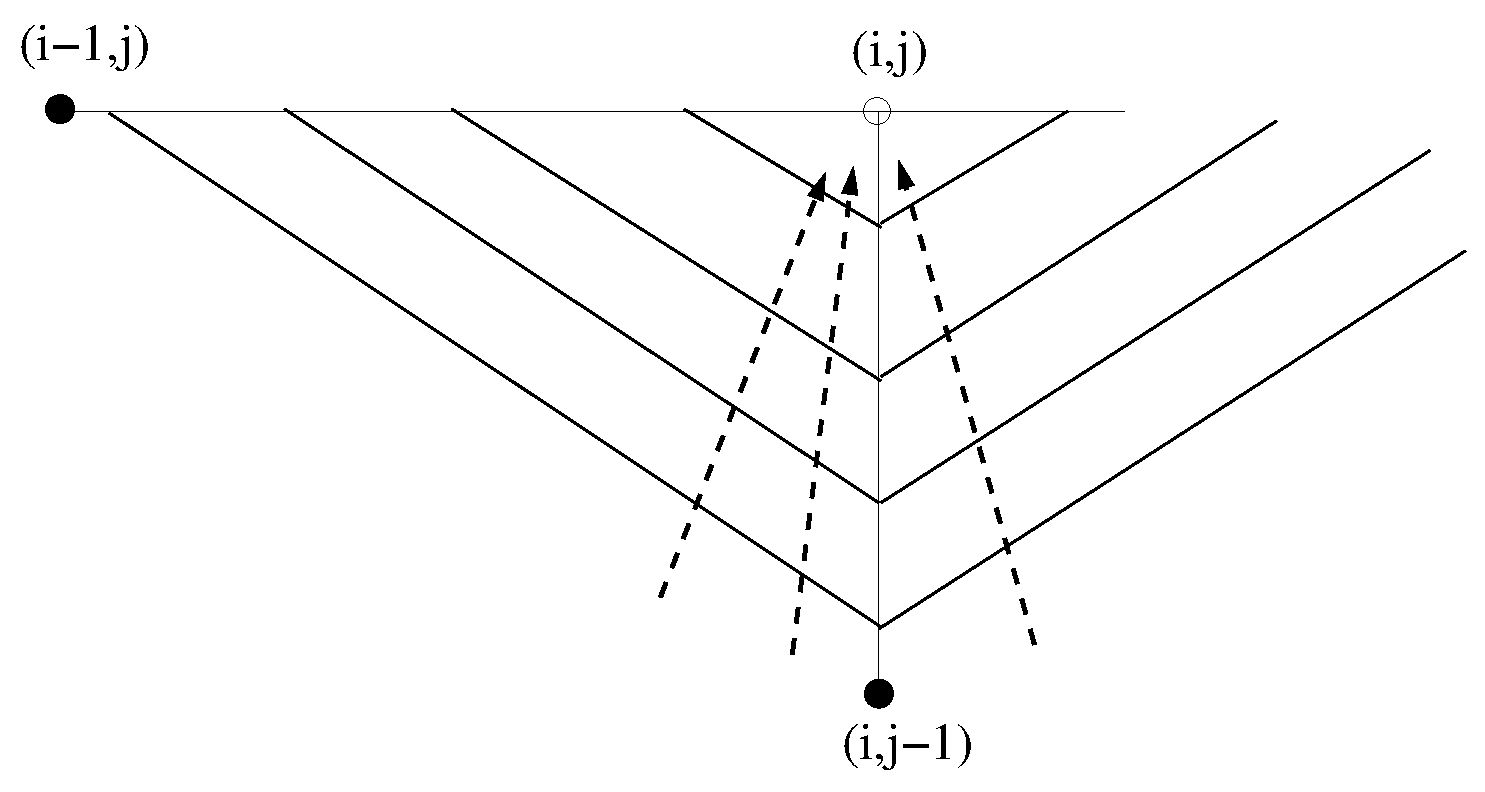
\epsfig{file=refrac.eps,height=6cm}
              }
      \caption{Geographic grid with parallel depth contours.}
      \label{fig:refr2}
\end{figure}
We assume that grid point $(i,j)$ is in shallow water. The other two grid points $(i-1,j)$ and $(i,j-1)$ are in deeper water.
Let $n$ be the coordinate along the wave rays.
Then according to Snel's law (Holthuijsen, 2007, NOTE 7A, pg. 207), we have
\begin{equation}
  \frac{d\theta}{dn} = \frac{1}{c}\frac{dc}{dn}\tan \theta\, .
\end{equation}
Here $\theta$ will be of the order of 45$^o$. So, we get
\begin{equation}
   \frac{d\theta}{dn} = \frac{1}{c}\frac{dc}{dn} \, .
\end{equation}
The slope at grid point $(i,j)$ determines the value of $d\theta/dn$. In shallow water, $c = \sqrt{gh}$, so
\begin{equation}
   \frac{d\theta}{dn} = \frac{1}{2h}\frac{dh}{dn} \, .
\end{equation}
This may be approximated as follows
\begin{equation}
  \frac{d\theta}{dn} \approx \frac{1}{2h_{i,j}}\frac{h_*-h_{i,j}}{\Delta n}
\end{equation}
with $h_*$ the water depth in one of the neighbouring grid points $(i-1,j)$ and $(i,j-1)$. In the numerical procedure $d\theta/dn$ is constant over a spatial step, so the change in direction over a step is
\begin{equation}
  \frac{d\theta}{dn} \Delta n = \frac{h_* - h_{i,j}}{2h_{i,j}} \, .
\end{equation}
In order to maintain stability the change of direction must remain below 90$^o$. Consequently, we obtain
\begin{equation}
  h_* - h_{i,j} \leq \pi h_{i,j} \, .
\end{equation}
In the program the factor $\pi$ is replaced by a user-determined factor $\beta$. Hence, the depths in surrounding grid points are reduced to $\beta h_{i,j}$, if they are larger than this value.
It should be noted that this approach was outlined in an unpublished note. Our experience with this approach is that it seems not effective enough.
\\[2ex]
Another try was given by Erick Rogers in the midsummer of 2007. His main motivation was refraction due to mud (non-rigid seafloor) which result in a dispersion relation that varies with $(x,y)$.
Currently, wave refraction can only be caused by depth variation (or current variation); see Eq. (\ref{eq:ctheta1}). As an alternative, the turning rate can be formulated in terms of wave
number as follows (see Holthuijsen, 2007, pg. 210, footnote 4)
\begin{equation}
    c_\theta = \frac{c_g}{k} \frac{\partial k}{\partial m}\, .
  \label{eq:ctheta2}
\end{equation}
The conjecture of Erick Rogers was that Eq. (\ref{eq:ctheta2}) differs from Eq. (\ref{eq:ctheta1}) due to numerics. His experiments suggested that Eq. (\ref{eq:ctheta2})
with coarse resolution yields results that are similar to those using Eq. (\ref{eq:ctheta2}) or Eq. (\ref{eq:ctheta1}) with high resolution. Though this seems to be the case with the
circular shoal case (matching a similar feature in the southern California Bight as descibed in \cite{Rog07KHJDH}), our general impression, however, is that this is generally not the case. The reason is that $\partial k/\partial m$ can be large as well,
if the bottom slope is large (not necessarily of the same order). Moreover, current gradients may also lead to an excessive wave refraction (i.e.
$c_\theta \sim -\vec{k}/|\vec{k}| \cdot \partial \vec{U}/\partial m$).
We have tried this approach for the Katrina hurricane at the Gulf of Mexico with an unstructured grid coupled to ADCIRC (Dietrich et al., 2011). The desired effect did not
show up, i.e. the excessive turning rate of waves at diverse locations remained during the whole simulation.

\chap{Wave boundary and initial conditions} \label{ch:bc}

To obtain the numerical solution of the action balance equation (\ref{eq:actbal1}), the wave boundary
and initial conditions should be provided. The incoming wave components at the up-wave
boundaries in the SWAN model are specified by a two-dimensional spectrum. Several
options are available:
\begin{itemize}
  \item A parametric one-dimensional spectrum with a certain imposed directional distribution.
        An example is a Jonswap spectrum.
  \item A discrete one-dimensional spectrum with a certain imposed directional distribution.
        This is often obtained from measurements.
  \item A discret two-dimensional spectrum. This may be obtained from other SWAN runs or other
        models, e.g. WAM and WAVEWATCH~III.
\end{itemize}
For the parametric one-dimensional spectrum, the following optional forms have been recommended:
a Pierson-Moskowitz spectrum (Pierson and Moskowitz, 1964), a Jonswap spectrum
(Hasselmann~{\it et~al}., 1973) and a Gaussian-shaped spectrum.
\\[2ex]
\noindent
The boundaries in frequency space are fully absorbing at the lowest and the highest discrete
frequency. So, energy can freely propagate across these boundaries and thus total energy
might not be conserved in some cases. However, a diagnostic tail $f^{-m}$ ($m=4$ or $m=5$)
is added above the high frequency cut-off, which is used to compute nonlinear wave-wave
interactions at the high frequencies and to compute integral wave parameters. When the directional
space is a closed circular, no directional boundary conditions are needed. However,
for reasons of economy, SWAN has an option to compute only wave components in a pre-defined
directional sector. In this case, the boundaries of this sector are fully absorbing (action
density might be removed from the model by refraction).
\\[2ex]
\noindent
To facilitate the integration process of the action balance equation, wave boundary conditions
in geographical space need to be provided. The boundaries of the computational grid in SWAN
are either land or water. In case of land there is no problem. The land does not generate waves
and in SWAN it absorbs all incoming wave energy. But in the case of a water boundary there is
a problem. If observations are available, they can be used as inputs at the boundary. In case
no wave conditions are given along the boundary, SWAN assumes that no waves enter the model
and waves can leave the model freely along that boundary. This assumption results in errors.
Therefore, to get reliable results, especially for such case, the model boundaries must be placed
far away from the area of interest.
\\[2ex]
\noindent
In case of nonstationary computation, the default initial spectra are computed from the local
wind velocities using the deep-water growth curve of Kahma and Calkoen (1992), cut off at values
of significant wave height and peak frequency from Pierson and Moskowitz (1964). The average
(over the model area) spatial step size is used as fetch with local wind. The shape of the
spectrum is default Jonswap with a $\cos^2 (\theta)$ directional distribution centred around
the local wind direction.
\\[2ex]
\noindent
The first guess conditions of a stationary run of SWAN are default determined with the second
generation mode of SWAN.
\\[2ex]
\noindent
It is possible to obtain an initial state by carrying out a previous stationary or nonstationary
computation.

\chap{Implementation of 2D wave set-up} \label{ch:setup}

\section{Methods} \label{sec:meth}

For the present purpose flows in shallow water are sufficiently described by the so-
called shallow-water equation which consists of one continuity equation and two
equations of motion (one for the $x-$ and one for the $y-$component). For the present
project the shallow water equation has to be simplified. The possibilities for such
simplification are investigated in the remainder of this section.
\\[2ex]
\noindent
Wave setup is usually confined to narrow zones in the immediate vicinity of the
shoreline. The size of such areas is small enough that the setup process can be
considered to be quasi-stationary.
\\[2ex]
\noindent
Wave-induced currents are usually weak compared with e.g. tidal currents.
Therefore it seems acceptable to neglect all terms in the equation of motion where
the current velocity appears.
\\[2ex]
\noindent
Comparisons of SWAN results with results from a full 2-dimensional flow model
have to show under which conditions the simplified equation provides acceptable
results. Such investigations are outside the scope of the present project. This report
presents a few cases with low overall current velocities where apparently the
computed setup is reasonably in accordance with expectations.
\\[2ex]
\noindent
Deleting from the equation of motion all terms involving current velocities we retain
an equilibrium between the wave-induced force and the gradient of the water table,
i.e.
\begin{equation}
F_{k} + gd \frac{\partial \zeta}{\partial x_{k}} = 0\;,
\label{eq:1N}
\end{equation}
where $\zeta$ is the setup, $d$ the depth and $F_{k}$ is the wave-induced force.
In a one-dimensional model (\ref{eq:1N}) can be used directly to compute the setup. In two
dimensions (\ref{eq:1N}) is a set of two equations with only one unknown,
the setup $\zeta$. In
order to reduce the number of equations to one, we use the observation by
Dingemans (1997) that wave-driven currents are mainly due to the
divergence-free part of the wave forces whereas the setup is mainly due to the
rotation-free part of the force field. We therefore take the divergence of eq. (\ref{eq:1N}) to
obtain the following elliptic partial differential equation for $\zeta$:
\begin{equation}
\frac{\partial F_{k}}{\partial x_{k}} + \frac{\partial}{\partial x_{k}}
(gd \frac{\partial \zeta}{\partial x_{k}}) = 0
\label{eq:2N}
\end{equation}
This Poisson equation needs one boundary condition in each point of the boundary
of the computational domain. Two types of boundary conditions are foreseen; the
first one is used on the open boundaries and on the shoreline where the shoreline
is defined as the line where the depth is zero:
\begin{equation}
F_{n} + gd \frac{\partial \zeta}{\partial n} = 0
\label{eq:3N}
\end{equation}
It is not possible to use this boundary condition on all boundary points because
then there remains an unknown constant. So on on point, for which we take the
boundary point with the largest depth the setup is assumed to be 0:
$\zeta=0$.
\\[2ex]
\noindent
The second type of boundary condition with given value of $\zeta$ is also used in nested
models. The setup computed in the larger model is used as boundary condition in
the nested model. In the nested model the setup  is given in all points of the outer
boundary. On shorelines inside the area again eq. (\ref{eq:3N}) is used.
\\[2ex]
\noindent
The Poisson equation (\ref{eq:2N}) together with its boundary conditions will be solved
numerically on a curvi-linear grid. The next section discusses the details of the
method, and presents some results of preliminary computations with the above
model.
\\[2ex]
\noindent
The actual design of the modifications of the SWAN commands is presented in
Appendix A, the design of the modifications of the code is presented in Appendix
B. After each iteration performed in SWAN new values of the setup are being
calculated and added to the depth, so that the SWAN model incorporates the effect
of setup on the wave field. An output quantity {\tt SETUP} is added so that the user can
be informed about the magnitude and distribution of the wave setup.
\\[2ex]
\noindent
\section{Analysis and Results}
\subsection{Discretization of the 2D setup equation}
\label{sec1G}
%
\subsubsection{Problem definition}
\label{subsec1.1G}
%
The equation to be solved has the following form:
\begin{equation}
\frac{\partial}{\partial x_{k}}(F_{k} + gd \frac{\partial \zeta}{\partial
x_{k}}) = 0\;,
\label{eq:1G}
\end{equation}
with $\zeta$ the setup, $d$ the depth and $F_{k}$ a golf-induced, time-averaged
force.\\
In order to solve (\ref{eq:1G}), the following types of boundary conditions
may be applied
\begin{equation}
F_{n} + gd \frac{\partial \zeta}{\partial n} = 0 \;\;\;\mbox{at the boundary}\;,
\label{eq:2G}
\end{equation}
with $n$ the outward direct normal. This is a so-called Neumann condition.
The setup is fixed upon an additive constant.
\begin{equation}
\zeta =\; \mbox{given at the boundary}\;.
\label{eq:3G}
\end{equation}
This is boundary condition of Dirichlet type.\\[2ex]
At beaches always the Neumann condition (\ref{eq:2G}) is applied.\\
In order to solve (\ref{eq:1G}) with boundary conditions (\ref{eq:2G}) and
(\ref{eq:3G}) a boundary fitted, vertex centered finite volume method is
applied. The discretization is based on the method described in
Van Beek~{\it et~al}. (1995).
In the remainder of this Chapter we use $k$ instead of $gd$.
%
\subsubsection{Discretization}
\label{subsec1.2G}
%
The physical domain is mapped onto a rectangular domain in the $(\xi^{1},
\xi^{2})$ plane, which is called the computational domain. All points of
the domain are used, including the dry ones.\\[2ex]
Using the relation Zijlema (1996) (summation convection applied):
\begin{equation}
\frac{\partial \varphi}{\partial x^{\beta}} = \frac{1}{\sqrt{g}}
\frac{\partial}{\partial\xi^{\gamma}}(\sqrt{g}\;  a^{(\gamma)}_{\beta}\;
\varphi)\;,
\label{eq:4G}
\end{equation}
with $a^{(\gamma)}_{\beta}$ the components of the contravariant basevectors
$\vec{a}^{(\alpha)}$ defined as (Segal~{\it et~al}, 1992):
\begin{equation}
\vec{a}^{(\alpha)} = \nabla \xi^{\alpha}\;,
\label{eq:5G}
\end{equation}
and $\sqrt{g}$ the Jacobian of the transformation:
\begin{equation}
\sqrt{g} = a^{1}_{(1)} a^{2}_{(2)} - a^{2}_{(1)}a^{1}_{(2)}\;.
\label{eq:6G}
\end{equation}
$\vec{a}_{(\alpha)}$ are the covariant base vectors defined by
\begin{equation}
\vec{a}_{(\alpha)} = \frac{\partial \vec{x}}{\partial \xi^{\alpha}} \; .
\label{eq:7G}
\end{equation}
The contravariant base vectors follow immediately from the covariant ones
due to:
\begin{eqnarray}
\sqrt{g}\vec{a}^{(1)}&=&(a^{2}_{(2)}, \; -a^{1}_{(2)})^{T}\;,\label{eq:8aG}\\
\sqrt{g}\vec{a}^{(2)}&=&(-a^{2}_{(1)}, \; a^{1}_{(1)})^{T}\;.\label{eq:8bG}
\end{eqnarray}
Application of (\ref{eq:4G}) to equation (\ref{eq:2G}) results in
\begin{equation}
\frac{1}{\sqrt{g}} \frac{\partial}{\partial \xi^{\alpha}}(\sqrt{g}
\vec{a}^{(\alpha)} \cdot (k \nabla \zeta + \vec{F})) = 0\;.
\label{eq:9G}
\end{equation}
Note that $\nabla \zeta$ is a derivative in the Cartesian $(\vec{x})$
direction and not in the $\vec{\xi}$ direction.\\[2ex]
In the remainder we shall use the local numbering as given in
Figure~\ref{fig1G}.
\begin{figure}[htb]
\centerline{\psfig{figure=fig1G.eps}}
\caption{Local numbering in computational domain}
\label{fig1G}
\end{figure}
The points (0, 0), (2, 0), (0, 2) and so on are the vertices of the cells.
The integration cell for the finite volume method is defined by the cell
$\Omega $ (-1, 0), (0, -1), (1, 0), (0, 1).\\[2ex]
Integrating (\ref{eq:9G}) over this cell gives
\begin{eqnarray}
&&\int\limits_{\Omega_{x}} \frac{1}{\sqrt{g}} \frac{\partial}{\partial
\xi^{\alpha}}(\sqrt{g} \vec{a}^{(\alpha)} \cdot (k \nabla \zeta +
\vec{F}))d\Omega_{x}\nonumber\\
&&\int\limits_{\Omega_{\xi}} \frac{\partial}{\partial
\xi^{\alpha}}(\sqrt{g}\vec{a}^{(\alpha)} \cdot (k \nabla \zeta
+ \vec{F}))d\Omega_{\xi}\label{eq:10G}\\
&&\approx \sqrt{g}\vec{a}^{(1)} \cdot (k\nabla \zeta + F)|^{(1,0)}_{(-1,0)}
+ \sqrt{g}\vec{a}^{(2)} \cdot (k \nabla \zeta + \vec{F})|^{(0,1)}_{(0,
-1)}\;,
\nonumber
\end{eqnarray}
where $\Omega_{x}$ is the cell in the physical space and $\Omega_{\xi}$ the
cell in the computational domain.\\
The four points (1, 0), (0, 1), (-1,0) and (0, -1) will be cell integration
points. The covariant basis vectors $\vec{a}_{(\alpha)}$ are approximated by
central differences.
\begin{eqnarray}
\vec{a}_{(2)}|_{(0,1)}&=&\vec{x}_{(0, 2)} - \vec{x}_{(0,0)}\;,\label{eq:11G}\\
\vec{a}_{(1)}|_{(1, 0)}&=&\vec{x}_{(2,0)} - \vec{x}_{(0,0)}\;,\label{eq:12G}
\end{eqnarray}
and by linear interpolation in other points.\\
In these relations we have used that the step width in the computational
domain is equal to 1.\\
The term $\nabla \zeta$ needs special attention. Since it concerns derivatives
in the $\vec{x}$ direction, whereas all derivatives in the computational
domain are in the $\vec{\xi}$ directions it is necessary to make some
approximation. We approximate this term by the integration path method
introduced in Van Beek~{\it et~al}. (1995).\\[2ex]
To that end $\nabla \zeta$ is integrated in two independent directions
$\xi^{1}$ and $\xi^{2}$. This yields two equations to express
$\frac{\partial \zeta}{\partial x}$ and $\frac{\partial \zeta}{\partial y}$ in
$\zeta$ values of neighbours.
\begin{eqnarray}
&&(\vec{x}_{2,0} - \vec{x}_{),0})\nabla \zeta|_{(1, 0)} = \zeta_{2,0} -
\zeta_{0,0}\;,\label{eq:13G}\\
&&\frac{1}{2}((\vec{x}_{2,2} - \vec{x}_{2,-2}) + (\vec{x}_{0,2} -
\vec{x}_{0,-2}))\nabla \zeta|_{(1,0)} = \frac{1}{2}((\zeta_{2,2} -
\zeta_{2,-2}) + (\zeta_{0,2} - \zeta_{0,-2}))\;.\label{eq:14G}
\end{eqnarray}
(\ref{eq:13G}), (\ref{eq:14G}) may be considered as two sets of equations
to express $\nabla \zeta$ into $\zeta$ values. Solution of this linear
system results in:
\begin{equation}
\nabla \zeta |_{(1,0)} = \zeta |^{(2,0)}_{(0,0)} \vec{c}^{(1)} +
(\zeta|^{(0,2)}_{(0, -2)} + \zeta |^{(2,2)}_{(2,-2)})\vec{c}^{(2)}\;,
\label{eq:15G}
\end{equation}
with
\begin{eqnarray}
\vec{c}^{1}&=&\frac{1}{C}(c^{2}_{(2)}, \; -c^{1}_{(2)})\; ; \; \vec{c}^{2} =
\frac{1}{C}(-c^{2}_{(1)}, \; c^{1}_{(1)})\;,\label{eq:16aG}\\
C&=&c^{2}_{(2)}c^{1}_{(1)} - c^{2}_{(1)}c^{1}_{(2)}\;,\label{eq:16bG}\\
\vec{c}_{(1)}&=&a_{(1)}|_{(1,0)}\; \; \vec{c}_{(2)} = \vec{a}_{(2)}|_{(0,-1)} +
\vec{a}_{(2)}|_{(0,1)} + \vec{a}_{(2)}|_{(2, -1)} + \vec{a}_{(2)}|_{(2,1)}\;.
\label{eq:16c}
\end{eqnarray}
A similar formula is applied for point (0, 1). Equation (\ref{eq:10G})
together with expression (\ref{eq:15G}) gives one row of the discretized
equation.
%
\subsubsection{Treatment of the boundary conditions}
\label{subsec1.3G}
%
The boundary conditions at the outer boundary of the domain are relatively
easy to implement.\\[2ex]
In case of Dirichlet boundary conditions the corresponding row of the
matrix is made equal to 0 and the diagonal element is set to 1. The value
of the boundary condition is filled into the right-hand side.\\[2ex]
Neumann boundary conditions are treated integrating over a half cell as
sketched in Figure~\ref{fig2G}.
\begin{figure}[htb]
\centerline{\psfig{figure=fig2G.eps}}
\caption{Half cell at boundary}
\label{fig2G}
\end{figure}
In this case we get:
\begin{eqnarray}
&&\int\limits_{\Omega_{\xi}}\frac{\partial}{\partial
\xi^{\alpha}}(\sqrt{g}\vec{a}^{(\alpha)} \cdot (k \nabla \zeta +
\vec{F})d\Omega_{\xi}\nonumber\\
&&\simeq\frac{1}{2}\sqrt{g}\vec{a}^{(1)} \cdot (k \nabla \zeta +
\vec{F})|^{(1,0)}_{(-1,0)} + \sqrt{g}\vec{a}^{(2)} \cdot (k \nabla \zeta +
\vec{F})|^{(0,1)}_{(0,0)}\;.
\label{eq:17G}
\end{eqnarray}
Due to the Neumann boundary conditions the term in the boundary point (0,
0) vanishes.\\[2ex]
Mark that in this case we need to evaluate $\nabla \zeta$ at the boundary.
In order to do so we apply a one-sided integration path approach i.e.
\begin{eqnarray}
&&(\vec{x}_{(2,0)} - \vec{x}_{(1,0)}) \cdot \nabla \zeta |_{(1,0)} =
\zeta_{(2,0)} - \zeta _{(0,0)}\;,\nonumber\\
&&((x_{(2,2)} - x_{(2,0)}) + (\vec{x}_{(0,2)} - \vec{x}_{(0,0)})) \cdot
\nabla \zeta |_{(1,0)} = (\zeta_{(0,2)} - \zeta_{(0,0)}) + (\zeta_{(2,2)} -
\zeta_{(2,0)})\;.
\label{eq:18G}
\end{eqnarray}
Furthermore we need the values of $\vec{a}_{(\alpha)}$ in virtual cells,
because we need the $c^{(\alpha)}$ at the boundary. To that end we
construct a row of virtual cells by extrapolating the co-ordinates of the
boundary cells.
%
\subsubsection{The implementation of dry points}
\label{subsec1.4G}
%
Dry points complicate the software considerably.\\[2ex]
For the dry points itself there is no problem. In fact we make the
corresponding row of the matrix, as well as the right-hand side element
completely equal to zero. This is allowed since our linear solver is able
to deal with zero rows.\\[2ex]
Dry points in the neighbourhood of wet points, however, also influence the
matrix for the wet point. Consider for example the integration point (1,0)
in Figure~\ref{fig3G}.
\begin{figure}[htb]
\centerline{\psfig{figure=fig3G.eps}}
\caption{Dry point (2, 0) and wet  point (0, 0)}
\label{fig3G}
\end{figure}
If (0, 0) is a wet point and (2, 0) a dry point then we assume that at
point (1,0) we have a Neumann boundary condition. This means in fact that
the contribution of the integration point (1,0) to the matrix and right-hand
side is equal to zero. With respect to the evaluation of the gradient of
$\zeta$ with the integration path method one sided differences are applied
for those formulas involving $\zeta_{(2,0)}$. This process is applied for
all transitions from wet to dry points. As a consequence, in the case of a
situation like in Figure~\ref{fig4G} we make $\nabla \zeta$ for point 2
zero.
\begin{figure}[htb]
\centerline{\psfig{figure=fig4G.eps}}
\caption{Wet points $\bullet$ enclosed by a row of dry points $\times$}
\label{fig4G}
\end{figure}
The reason is that in point 2 it is only possible to evaluate
$\frac{\partial \zeta}{\partial \xi^{1}}$ and not $\frac{\partial
\zeta}{\partial \xi^{2}}$, and hence we have too few information to express
$\nabla \zeta$ in neighbour values.
%
\subsubsection{Building of the matrix and right-hand side}
\label{subsec1.5G}
%
With respect to the building of matrix and right-hand side we start by
computing all contributions in the integration points. This is done by
looping over the various integration points. Since the contribution of
point (0,1) in cell $(i, j)$ is equal to that of point (0, -1) in cell
$(i-1,j)$ it is sufficient to loop over two sets of integration points
only.\\[2ex]
Once we have computed the coefficients in a set of integration points we
must add these contributions, multiplied by some factor, to the matrix
elements. This process is known as distribution.\\[2ex]
Hence the actual implementation is as follows:
\begin{itemize}
\item[1] Map indirect addressing to direct addressing. (subroutine swdct).
\item[2] Compute and store $\vec{a}_{(\alpha)}$ for all integration points.
First we use central differences where possible and after that we apply
linear interpolation for the remaining points. (subroutine swcova2d).
\item[3] Compute $\sqrt{g}\vec{a}^{(\alpha)}$ in all integration points using
$\vec{a}_{(\alpha)}$. (subroutine swjcta2d).
\item[ ] For 2 integration directions do
 \begin{itemize}
 \item[4] Compute factors $\vec{c}^{(\alpha)}$ taking into account boundary
 effects and dry points.\\
 Compute contributions for matrix and right-hand side for integration
 points.\\
 (subroutine swtrad2d).
 \item[5] Distribute contribution to correct matrix elements.\\
 (subroutine swdisdt2).
 \end{itemize}
\item[6] Fill essential boundary conditions.\\
(subroutine swessbc).
\item[7] Solve system of linear equations.\\
(subroutine swsolve).\\
This part is explained in more detail in the next Chapter.
\item[8] Map from direct to indirect addressing.\\
(subroutine swindct).
\end{itemize}
%input{discretization}
% stuk van Kees V.
\subsection{The iterative solver for the linear system}
In this section we describe the mathematical methods, which are used to
solve the system of linear equations as derived in Chapter 1. In
Section \ref{sec:data} we consider the data structure used.
Some properties of the matrix are given in Section \ref{sec:prop}.
Due to the sparseness of the matrix we prefer an iterative solution
method of Krylov subspace type. The details are described in Section
\ref{sec:iter}.
As is well known, Krylov subspace methods are only attractive when
they are combined with suitable preconditioners (see Section
\ref{sec:prec}). Finally our choices are summarised in Section
\ref{sec:sum}.
\subsubsection{Data structure}
\label{sec:data}
After the discretization of the Poisson equation in curvi-linear
co-ordinates, one has to solve the following matrix vector system:
\begin{equation}
A x = f,
\label{eq:matvec}
\end{equation}
where $A$ is the discrete Poisson operator, $x$ is an approximation of
the setup (of the water level), and the right-hand-side vector $f$
contains the effects of the boundary conditions and the forces due to
the surface waves. In the solver it is very efficient to calculate with
direct addressing, so dry points are included in the vector $x$. This
implies that the dimension of $x$ and $f$ are fixed and equal to $MXC
\times MYC$. In the discretization a 9-point stencil is used.  That
implies that only 9 matrix elements per row are non-zero. These elements
are stored in a diagonal-wise way.  So for this part $NWKARR = 9$. The
rows corresponding to dry points are filled with zeroes except on the
main diagonal where the value 1 is substituted. The value of $x$ and $f$
are taken equal to 0 at these points.
\subsubsection{Properties of the matrix}
\label{sec:prop}
The discrete operator is symmetric in the inner region. This means that
$a_{i,j} = a_{j,i}$. Due to the boundary conditions the symmetry of the
operator is lost. The reasons for this are:
\begin{itemize}
\item When Dirichlet boundary conditions are used the known elements of
$x$
should be eliminated in order to keep the matrix symmetric. However this
leads to a different dimension of $A, x,$ and $f$, therefore the known
elements are not eliminated.
\item When dry points occur the derivation of the discrete boundary
conditions is already complicated at the interface between wet and dry
points. At this moment it is not clear how to discretize these
conditions such that the resulting matrix is symmetric.
\end{itemize}
These difficulties motivate us to use a non-symmetric matrix. This is
only a small drawback, because recently good methods have
been developed to
solve non-symmetric matrix vector systems.\\[2ex]
When Neumann conditions are used on all boundaries the resulting matrix
is singular. The solution is determined up to a constant. We have to
keep this in mind during the construction of the solution
procedure.\\[2ex]
When Gauss elimination is used to solve equation (\ref{eq:matvec}), the
zero elements in the bend of $A$ become non-zero. This means that the
required memory is equal to $2 \times MXC  + 2$ vectors.
For $MXC$ large, this leads to an unacceptable large amount of memory.
Therefore we use an iterative solution method, where the total amount of
memory is less than the memory used in the discretization procedure.
\subsubsection{The iterative solver} \label{sec:iter}

In 1D cases, the wave-induced set-up is calculated in SWAN with a simple
trapezoidal rule.
\\[2ex]
\noindent
In 2D cases, the Poisson equation of the divergence-free force field is solved in
SWAN with a modified Successive Over Relaxation (SOR) technique (Botta and Ellenbroek, 1985).
The boundary conditions for this elliptical partial differential equation are:
\begin{itemize}
  \item at open boundaries: equilibrium between wave force and hydrostatic pressure gradient
        normal to the model boundary,
  \item at last grid points before shoreline: equilibrium between wave force and hydrostatic
        pressure gradient normal to the model boundary and
  \item at deepest boundary point: set-up is zero.
\end{itemize}
The shoreline in SWAN moves as dictated by the wave-induced set-up. The set-up computations are
available in both the recti-linear and curvi-linear grids.
\nocite{Bot85E}

\chap{Iterative solvers} \label{ch:solver}

\section{Strongly Implicit Procedure (SIP)}

We want to solve the following linear system of equations
\begin{equation}
  A \, \vec{N} = \vec{b}
\end{equation}
where $A$ is some non-symmetric penta-diagonal matrix, $\vec{N}$ is the wave action vector to be solved and $\vec{b}$
contains source terms and boundary values.

The basis for the SIP method (Stone, 1968; Ferziger and Peri\'{c}, 1999) lies in the observation that an LU decomposition is an excellent
general purpose solver, which unfortunately cannot take advantage of the sparseness of a
matrix. Secondly, in an iterative method, if the matrix $M = LU$ is a good approximation to the
matrix $A$, rapid convergence results. These observations lead to the idea
of using an approximate LU factorization of $A$ as the iteration matrix $M$, i.e.:
\begin{equation}
   M = L\,U = A + K
  \label{eq:lusip}
\end{equation}
where $L$ and $U$ are both sparse and $K$ is small. For non-symmetric matrices the incomplete LU
(ILU) factorisation gives such an decomposition but unfortunately converges rather slowly. In
the ILU method one proceeds as in a standard LU decomposition. However, for every element
of the original matrix $A$ that is zero the corresponding elements in $L$ or $U$ is set to zero. This
means that the product of $LU$ will contain more nonzero diagonals than the original matrix $A$.
Therefore the matrix $K$ must contain these extra diagonals as well if Eq. (\ref{eq:lusip}) is to hold.

Stone reasoned that if the equations approximate an elliptic partial differential equation the
solution can be expected to be smooth. This means that the unknowns corresponding to
the extra diagonals can be approximated by interpolation of the surrounding points. By
allowing $K$ to have more non zero entries on all seven diagonals and using the interpolation
mentioned above the SIP method constructs an LU factorization with the property that for a
given approximate solution $\phi$ the product $K\phi \approx 0$ and thus the iteration matrix $M$ is close to
$A$ by relation (\ref{eq:lusip}).

To solve the system of equations the following iterations is performed,
starting with an initial guess for the wave action vector ${\vec{N}}^0$ an iteration is performed solving:
\begin{equation}
   U\,{\vec{N}}^{s+1}  = L^{-1}\,K\,{\vec{N}}^s + L^{-1}\,\vec{b}
\end{equation}
Since the matrix $U$ is upper triangular this equation is efficiently solved by back substitution.
An essential property which makes the method feasible is that the matrix $L$ is easily
invertible. This iterative process is repeated $s=0,1,2,...$ until convergence is reached.

\section{Successive Over Relaxation (SOR) technique}
This section is under preparation.
See also Botta and Ellenbroek (1985).

\chap{Parallel implementation aspects} \label{ch:parall}

Domain decomposition methods have been successfully used for solving large sparse
systems arising from finite difference or finite volume methods in computational
fluid dynamics on distributed memory platforms. They are based, in essence, upon a
partition of the whole computational domain in $\vec{x}$-space into a number of contiguous,
non-overlapping subdomains with each of them being assigned to a different processor.
In this case the same algorithm performs on all available processors and on its own
set of data (known as the SPMD programming model). Each subdomain can have multiple
neighbors on each of its four sides. For this, a data structure is implemented to
store all the information about the relationship of the subdomain and its particular
neighbors. Next, each subdomain, look in isolation, is then surrounded by an auxiliary
layer of one to three grid points originating from neighbouring subdomains. This layer
is used to store the so-called halo data from neighbouring subdomains that are needed
for the solution within the subdomain in question. The choice of one, two or three grid
points depends on the use of propagation scheme in geographical space, i.e., respectively,
BSBT, SORDUP or Stelling/Leendertse. Since, each processor needs data that resides in
other neighbouring subdomains, exchange of data across boundaries of subdomains is
necessary. Moreover, to evaluate the stopping criterion (\ref{eq:stop}), global
communication is required. These message passings are implemented by a high level
communication library such as MPI standard. A popular distribution is MPICH
which is free software\footnote{Available from \hl{http://www-unix.mcs.anl.gov/mpi/mpich}.} and
is used in the present study. Only simple point-to-point and collective communications have
been employed. There are, however, some other implementation and algorithmic issues that
need to be addressed.
\nocite{Gro99LS}

\section{Load balancing} \label{sec:loa}

The mapping of subdomains on processors should be chosen so as to distribute
the computational load as equally as possible and to minimize the communication
cost. Intuitively, it will be clear that we have to allocate contiguous blocks
of equal numbers of grid points on each processor. However, in the context of
SWAN applications to coastal areas, some difficulties arise. Firstly, wet and
dry grid points may unevenly distributed over subdomains while no computations
have to be done in dry points. Secondly, an unbalanced partition may arise
during the simulation due to the tidal effect (dry points become wet and vice
versa). In such a case, one may decide to adapt the partition such that it is
balanced again (so-called dynamic load balancing). Finally, most end-users are
not willing to determine the partitioning themselves, thus automatic support
for partitioning the grids is desirable.

In the present study, two well-established partition methods are applied. The
first is called stripwise partitioning in which the computational grid is cut
along one direction, resulting in horizontal or vertical strips. The choice of
cutting direction depends on the interface size of the strips which should be
minimized. However, the communication volume, which is related to the total size
of the interfaces, can be further reduced by means of recursive application of
alternately horizontal and vertical bisection. This is known as Recursive
Co-ordinate Bisection (RCB). Further details on these techniques and an overview
on grid partitioning can be found, e.g. in Fox (1988) and Chrisochoides~{\it et~al}. (1994).
\nocite{Fox88,Chr94HR}.

Within SWAN, the grid partitioning is carried out automatically on wet grid points
only. The size of the subdomain equals the total number of wet points divided by
the total number of subdomains. The implementation of a stripwise partitioning is
as follows. First, an empty strip is created. Next, assign point-by-point to the
created part until the size of that part has been reached. Thereafter, verify
whether non-assigning wet points remain in the current strip. If so, these points
will be assign to the same part too, otherwise create next empty strip. As a result,
all strips have straight interfaces and include approximately the same number of wet
grid points. Moreover, experiences with SWAN simulation have shown that the amount
of computations in each wet grid point remains more or less constant during the
simulation and hence, there is no need for dynamic load balancing.

A final remark has to be made considering grid partitioning. The above described
methodology does not seem to have been implemented in spectral wave models before.
In Tolman (20020, another way of distributing data over the processors is discussed:
each $p^{\rm th}$ wet grid point is assign to the same processor with $p$ the total
number of processors. The requirement of equal numbers of wet grid points per processor
is provided automatically. However, it is impossible to compute the spatial wave
propagation in an effective manner. The only alternative is to gather data for all
grid points in a single processor before the calculation is performed. This will
require a full data transpose, i.e. rearranging data distribution over separate
processors. It is believed that this technique requires much more communication between
processors than domain decomposition and therefore less suitable for SWAN.

\section{Parallelization of implicit propagation schemes} \label{sec:imp}

Contrary to explicit schemes, implicit ones are more difficult to parallelize, because of
the coupling introduced at subdomain interfaces. For example, concerning the four-sweep
technique, during the first sweep, an update of $N(i,j,l,m)$ can be carried out as soon as
$N(i-1,j,l,m)$ and $N(i,j-1,l,m)$ have been updated and thus it can not be performed in
parallel. Parallelization of this implicit scheme requires modifications. Ideally, the
parallel algorithm need no more computing operations than the sequential one for the same
accuracy.

The simplest strategy to circumvent this problem consists in treating the data on subdomain
interfaces explicitly, which in mathematical terms amounts to using a block Jacobi
approximation of the implicit operator. In this context, we employ the RCB partition method,
since it gives the required balanced, low-communication partitioning. This strategy possess
a high degree of parallelism, but may lead to a certain degradation of convergence properties.
However, this numerical overhead can be reduced by colouring the subdomains with four different
colors and subsequently permuting the numbering of unknowns in four sweeps in accordance with
the color of subdomains. Furthermore, each subdomain is surrounded by subblocks of different
colors. See Figure~\ref{fig:colb}. As a result, each coloured subdomain start with a different
\begin{figure}[htb]
   \centerline{
      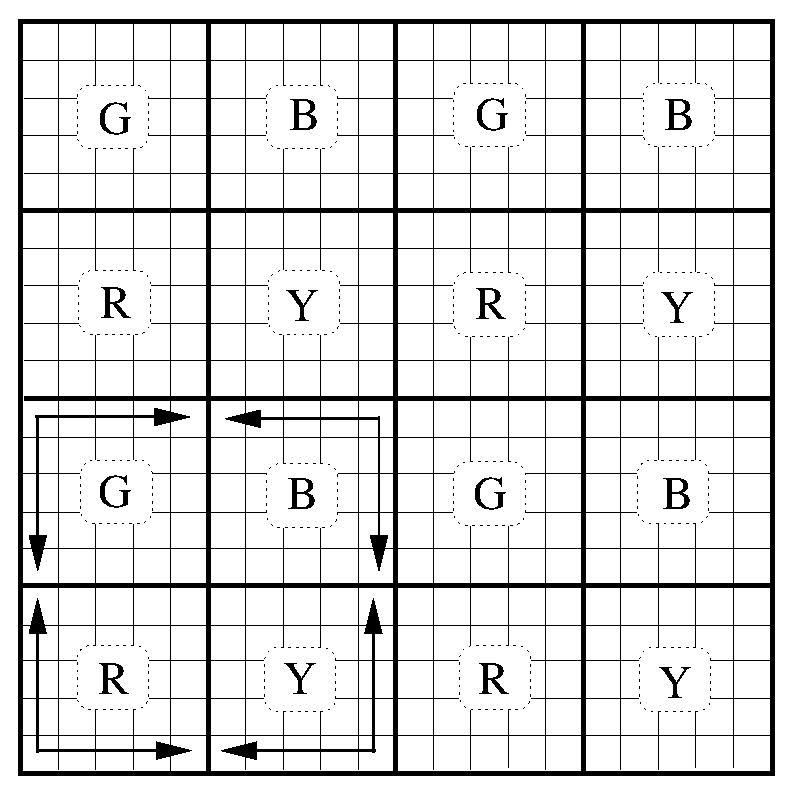
\epsfig{file=colblk.eps,height=7cm}
              }
      \caption{Four types of subblocks (red, yellow, green and black) treated differently
               with respect to the ordering of updates (indicated by arrows) per sweep.}
      \label{fig:colb}
\end{figure}
ordering of updates within the same sweep and thus reducing the number of synchronization
points. This multicolor ordering technique has been proposed earlier, e.g. in Meurant (1988)
and Van der Vorst (1989).

Another strategy is based on the ideas proposed by Bastian and Horton (1991) and is
referred here to as the block wavefront approach. It is demonstrated with the following
example. First, we decompose the computational domain into a number of strips. In this
example, we assume that these strips are parallel to $y-$axis. Next, we start with the
first sweep. The processor belonging to the first strip updates the unknowns $N(i,1,l,m)$
along the first row $j=1$. Thereafter, communication takes place between this processor and
processor for strip 2. The unknowns $N(i,2,l,m)$ along $j=2$ in strip 1 and $N(i,1,l,m)$ along
$j=1$ in strip 2 can be updated in parallel, and so on. After some start-up time all processors
are busy. This is depicted in Figure~\ref{fig:wfront}. Finally, this process is repeated
\begin{figure}[htb]
   \centerline{
      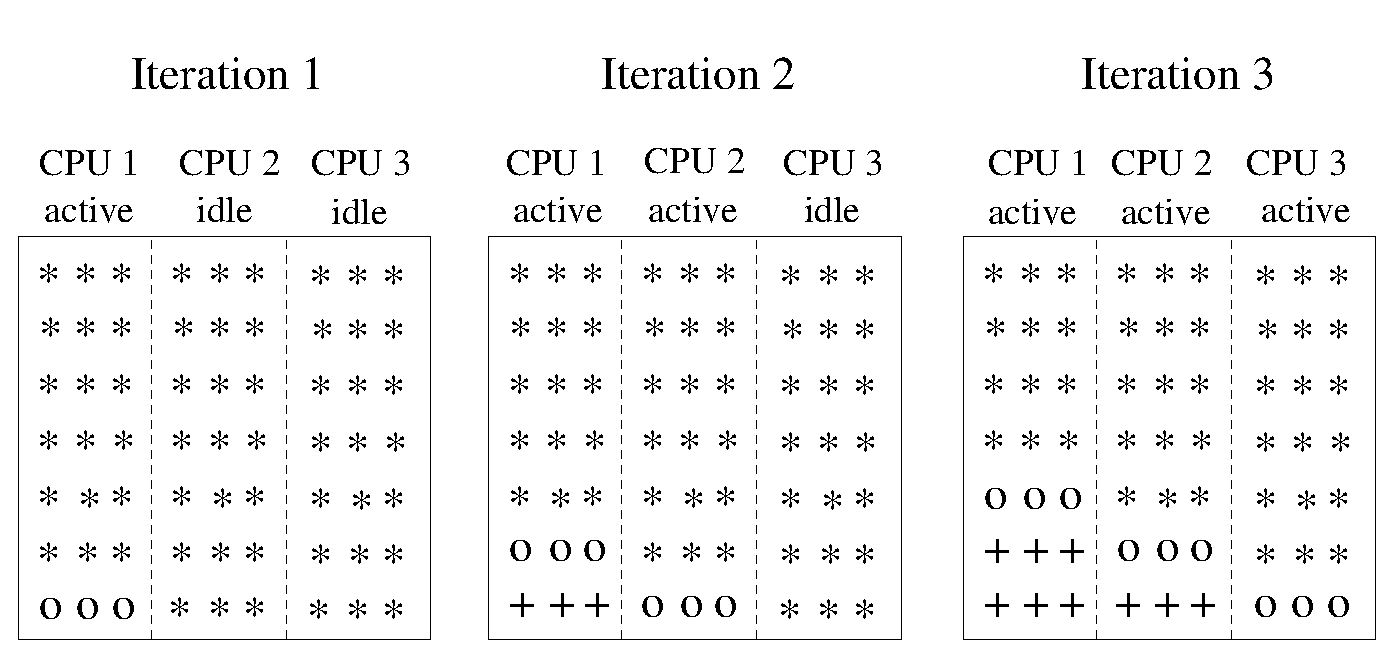
\epsfig{file=wavefront.eps,height=6cm}
              }
      \caption{Application of block wavefront approach for the first 3 iterations during the
               first sweep. Domain is divided into 3 vertical strips. Stars represent unknowns
               to be updated, circles mean that unknowns are currently updated and the plus
               signs indicate unknowns that have been updated.}
      \label{fig:wfront}
\end{figure}
for the other three sweeps. Details can be found in the source code of SWAN 40.20. The block
wavefront approach does not alter the order of computing operations of the sequential algorithm
and thus preserving the convergence properties, but reduces parallel efficiency to a lesser
extent because of the serial start-up and shut-down phases (Amdahl's law). This technique
resembles much to the standard wavefront technique applied in a pointwise manner (unknowns on
a diagonal are mutually independent and thus can be updated in parallel; for details, see
Templates (1994), which has also been employed by Campbell~{\it et~al}. (2002) for
parallelizing SWAN using OpenMP.
\nocite{Templates94,Cam02R}

The performance of the two discussed parallelization methods applied in the SWAN model has been
discussed in (Zijlema, 2005).
Numerical experiments have been run on a dedicated Beowulf cluster with a real-life application.
They show that good speedups have been achieved with the
block wavefront approach, as long as the computational domain is not divided into too thin slices. Moreover,
it appears that this technique is sufficiently scalable. Concerning the block Jacobi method, a considerable
decline in performance has been observed which is attributable to the numerical overhead arising from doubling
the number of iterations. Furthermore, it may result in a solution that is computed to an accuracy that may not
be realistic. In conclusion, parallelization with the block wavefront technique has been favoured and has been
implemented in the current operational version of SWAN.

A survey of other alternatives to the parallelization of the implicit schemes is given in Templates (1994).

\chap{Unstructured mesh implementation} \label{ch:unswan}

Since, the characteristic spatial scales of the wind waves propagating from deep to shallow waters are very
diverse, a flexible grid would be required to allow local refinement of the mesh
in areas of interest  e.g.,
regions of strong bathymetry variations in estuaries and fjords,
without incurring
overhead associated with grid adaptation at some distance offshore. Traditionally, this can be achieved by employing
a nesting technique.
Although, this practise is very common for SWAN, it is generally recognized that
this may lead to complicated programming with the corresponding significant increase in computational effort.

The use of unstructured grids, however, offers a good alternative to nested models not only because of the
ease of local grid refinement, either adaptive or fixed, but also the high flexibility to generate
grids along coastline and around islands.
The variable mesh is especially useful in coastal regions where the water depth varies greatly.
Thus, the variable grid gives the highest resolution where it is most needed.
Moreover, this can be automated to a large extent.
Although, the CPU cost per grid point is often relative higher than cases with structured grids,
this effect is probably more than offset by the reduction in the number of grid points.

This chapter presents an unstructured grid procedure for SWAN. Details can also be found in (Zijlema, 2009, 2010).
The numerical propagation scheme for structured grids is based on
a four-direction Gauss-Seidel iteration technique and is accompanied by a fully implicit temporal discretization; see Section~\ref{sec:sol}.
Hence, SWAN is stable for any time step.
Because of this nice property, this solution technique is tailored to unstructured grids.
\nocite{Zij09,Zij10}

\section{Description of an unstructured grid}
\label{sec:defunstr}

\subsection{Definitions}

We distinguish between two types of grids, namely structured and unstructured grids. A two-dimensional structured grid may contain quadrilaterals. These
can be recti-linear or curvi-linear. The number
of cells that meet each other in an internal vertex is always 4. In unstructured meshes this restriction is abandoned. Moreover, 2D unstructured grids usually
consist of triangles or a combination of triangles and quadrilaterals, a so-called hybrid grid. The unstructured meshes that we consider in SWAN consist solely
of triangles, also called cells. The edges of the triangles are called faces.

\subsection{Relations between number of cells, vertices and faces}

For a two-dimensional triangular mesh, the number of cells $C$, the number of boundary faces $E_b$ and internal faces $E_i$ are related according to:
\begin{equation}
  E_b + 2 E_i = 3C
\end{equation}
The total number of faces $E = E_i + E_b$. With $V$ the number of vertices and $H$ the number of holes ('islands'), we have the following Euler's relation
for a triangulation:
\begin{equation}
  C + V  - E = 1 - H
\end{equation}
Usually, $E_b << E_i$ and the number of holes $H$ is negligibly small, so
\begin{equation}
  C \approx 2V\, , \quad E \approx 3V
\end{equation}
There are approximately twice as many cells as vertices
in a triangular mesh.
Therefore, it is an optimal choice to locate the action density in vertices
as the number of unknowns is minimal on a given grid.
Concerning the
time-consuming evaluation of the physical processes representing the wave energy generation,
dissipation and redistribution, this allows SWAN to save a considerable amount of computing time.

\subsection{Conditions imposed to the grid}

In order to avoid badly shaped grids, the grids must satisfy the following
properties:
\begin{itemize}
  \item The number of cells that meet at each vertex in the interior of the mesh must be at least 4 and at most 10.
  \item The angles inside each triangle must be smaller than a certain value. Let $\vec{a}$ and $\vec{b}$ be the tangential vectors of two faces of a
        triangle, then the angle $\phi$ between these two faces equals
        \begin{equation}
           \cos \phi = \frac{\vec{a} \cdot \vec{b}}{|\vec{a}||\vec{b}|}
        \end{equation}
        For safety, we do not allow for angles with $\cos \phi < -0.8$ or, equivalently, $\phi > 143^o$.
\end{itemize}

\section{Some notes on grid generation}

We briefly outline some issues related to grid generation from a practical point of view.
The process of grid generation can be difficult and time consuming. A common approach is proceeding from coarse to fine grid through refinement in various ways.
Generally, one would like to have an optimal grid in which areas where the bathymetry or evolution of the waves change
rapidly require a higher resolution than areas where the physics or depth changes less.
This goes around by having an indication how to determine the refinement based on
bathymetry or geometric variations through preliminary evaluations.
To facilitate this procedure,
a mesh generation package BatTri (Bilgili and Smith, 2003) is used.
This grid generator is a public-domain, graphical Matlab interface to Triangle (Shewchuk, 1996).
Triangle is a freely-distributed, two-dimensional Delaunay triangulator.
\nocite{Bil03S,She96}

An important key ingredient for the preparation of the grid for the model domain is bathymetry data.
Boundary nodes, segments and holes
can be created from this data with the
use of the mesh editing options of BatTri.
After checking and improving grid quality, the final information on nodes and segments is forced into the
triangulation of the domain. Triangle is called within BatTri to generate
the actual grid. This triangulation includes only acute triangles.

BatTri provides many pre-defined depth-dependent contraints for further mesh refinement.
From a numerical point of view, mesh refinement is often directly related to properly resolve the shape of the wave,
i.e. to keep the wavelength to grid size ratio relatively large.
When wavelength decreases in shallower water, the grid size must decrease as well. Therefore, this criterion, called the $h$-refinement,
has the effect of using smaller cells in shallow water and larger
cells in deeper water. Here, $h$ refers to the water depth. Another useful criterion is known as the topographic length scale constraint,
when one try to keep the ratio $\Delta h/h$ less than one. Here, $\Delta h$ equals the difference between the maximum depth of a triangle and the minimum depth and
$h$ is the average depth. This
criterion addresses the bathymetric slope and cells with a high value of $\Delta h/h$ indicate areas of steep bottom topography that will need to be
more finely resolved.
When refining the grid, one must balance the need to fully meet the refinement criteria with the desire to keep the triangle sizes from becoming too small.
Thus, these criteria
are generally imposed along with a minimum area constraint.
The refinement process is repeated iteratively until a final grid with the appropriate resolution is obtained.

\section{Numerical method}
\label{sec:nummeth}

\subsection{Discretization procedure}

For the sake of clarity of the algorithm description below, we put all the terms but the time derivative and propagation term in the geographical space of Eq. (\ref{eq:actbal1})
in one term $F(\vec{x},\sigma,\theta)$:
\begin{equation}
  \frac{\partial N}{\partial t} + \nabla_{\vec{x}} \cdot [\vec{c}_{\vec{x}} N] = F
  \label{eq:waveeq}
\end{equation}
with $\vec{c}_{\vec{x}} = {\vec{c}}_g + \vec{U}$ the geographic velocity vector.

For the time being, we restrict ourselves to triangular meshes. However, other
type of meshes can be employed as well, e.g. hybrid grids (consisting of both triangles and quadrilaterals). We consider a triangulation of a geographical domain in which
Eq. (\ref{eq:waveeq}) is solved; see Fig~\ref{fig:triangul}.
\begin{figure}[htb]
   \centerline{
      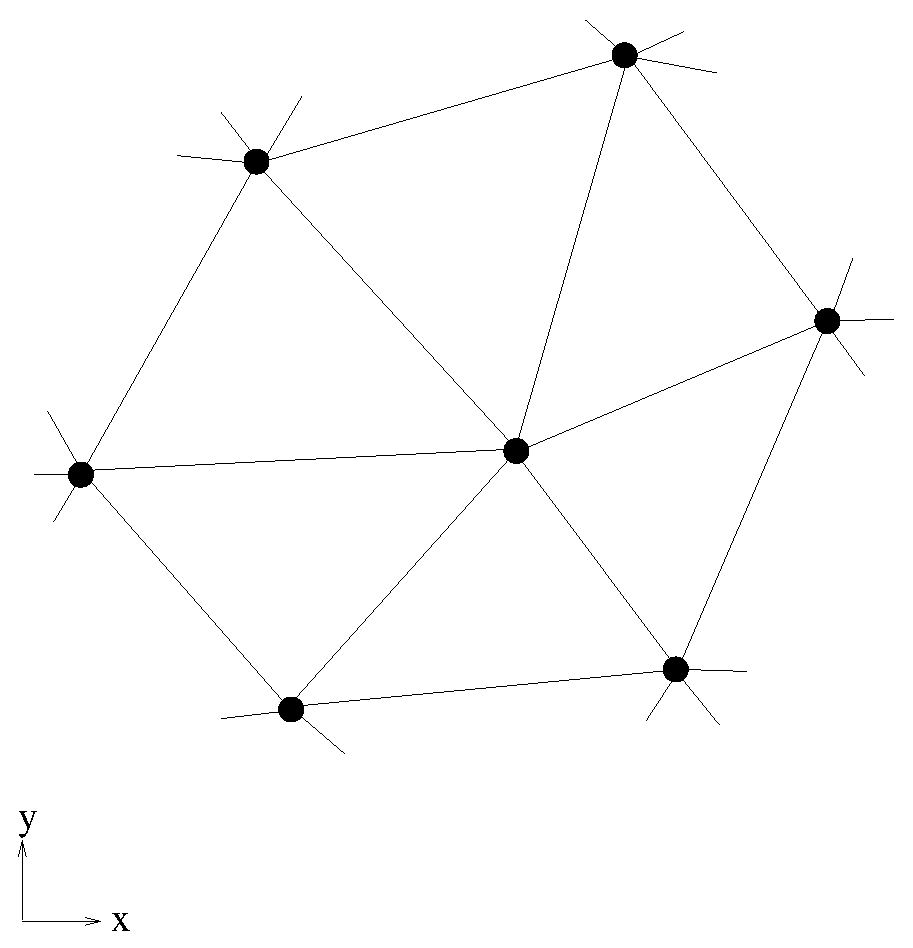
\epsfig{file=triangul.eps,height=7cm}
              }
      \caption{An example of triangulation.}
      \label{fig:triangul}
\end{figure}
Every vertex and all the triangles around this vertex are taken into account.
Observe that the number of cells around a vertex can be different for all vertices.
A vertex-based scheme is used in which the wave action $N$ is stored at the vertices and Eq. (\ref{eq:waveeq}) is solved in each vertex.
We note that the values at boundary vertices are fixed during the computation.

For the time integration, we adopt the first order implicit Euler scheme, as follows
\begin{equation}
  \frac{N^n - N^{n-1}}{\Delta t} + \nabla_{\vec{x}} \cdot [\vec{c}_{\vec{x}} N^n] = F^n
  \label{eq:waveeq2}
\end{equation}
where $\Delta t$ is the time step and $n$ is the time step counter. The main property of this approximation is that it does not suffer from the stability restriction
imposed by the CFL condition inherent in the explicit methods as employed in most spectral models. In principle, the time step is limited only by
the desired temporal accuracy. This procedure, however, involves the solution of a large system of equations.

A point-by-point multi-directional Gauss-Seidel iteration technique is employed for updating all grid vertices.
A key feature of this technique is that it takes advantage of the newly acquired vertex values during an iteration.
It is locally implicit but globally explicit. In other words, it circumvents the need to build or store large matrices and remains stable at any time steps.
This means that this numerical procedure can converge to steady state much more rapidly than
explicit methods without requiring too much computational work and memory as do implicit methods.

We consider the update of a vertex as labeled 1 in Figure~\ref{fig:gsunstruc}. This involves looping over each cell of this vertex.
\begin{figure}[htb]
   \centerline{
      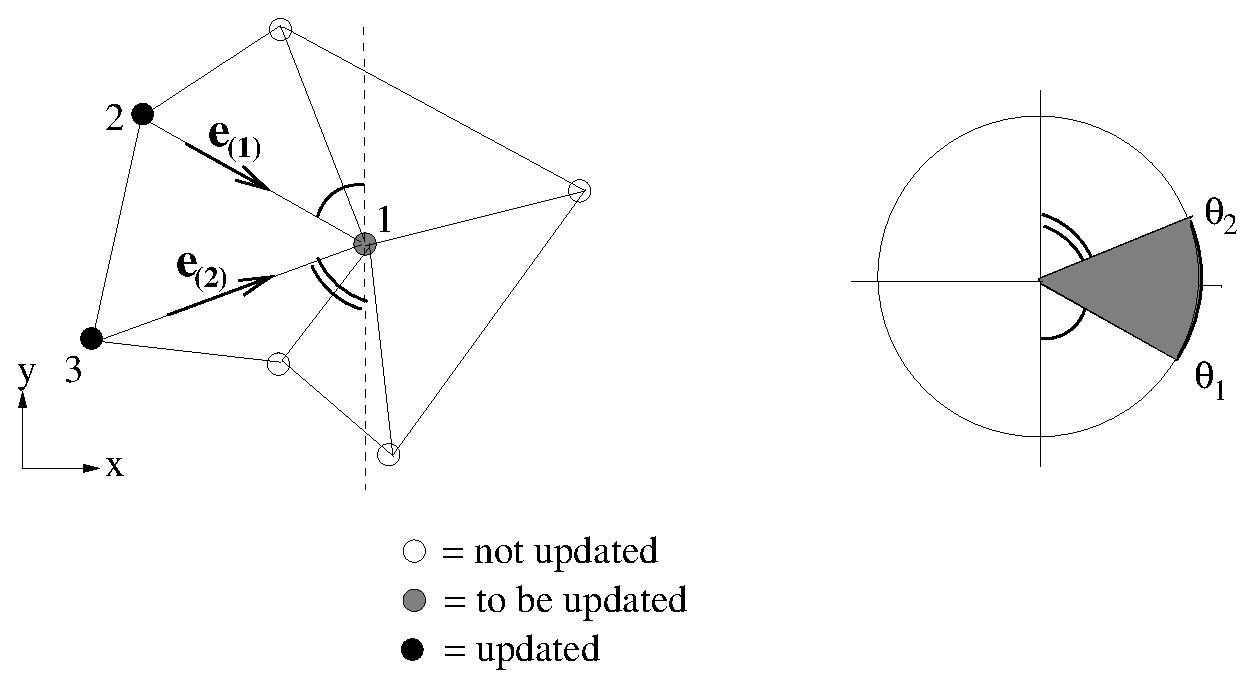
\epsfig{file=gsunstruc.eps,height=7cm}
              }
      \caption{Update of the wave action at vertex 1 in a triangle $\triangle$123 and the shaded directional sector
               in spectral space for which the waves are propagated.}
      \label{fig:gsunstruc}
\end{figure}
We want to find an approximation for the propagation term of Eq. (\ref{eq:waveeq2}). To this end, we employ some vector calculus.
We consider a triangular cell as depicted in Figure~\ref{fig:celldisc}.
\begin{figure}[htb]
   \centerline{
      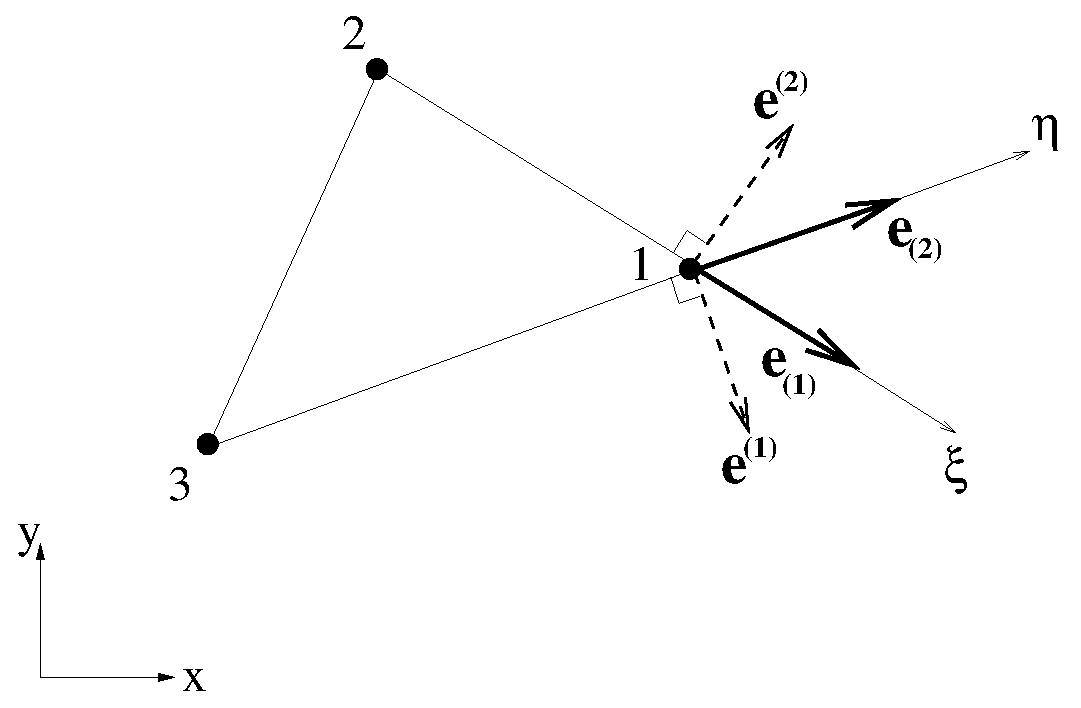
\epsfig{file=celldisc2.eps,height=8cm}
              }
      \caption{A triangular cell with geometrical quantities used for discretization in geographical space. Definitions of these quantities are provided in the text.}
      \label{fig:celldisc}
\end{figure}
In vertex 1, we apply a mapping from a local coordinate system $\vec{\xi}$ = ($\xi$,$\eta$) to the
Cartesian one $\vec{x}$ = ($x$,$y$).
Based on this transformation $\vec{x}(\vec{\xi})$, we have the following base vectors that are tangential to the coordinate lines $\xi$ and $\eta$, respectively,
\begin{equation}
  {\vec{e}}_{(1)}  = \frac{\partial \vec{x}}{\partial \xi} \, , \quad {\vec{e}}_{(2)}  = \frac{\partial \vec{x}}{\partial \eta} \, .
\end{equation}
The vectors
\begin{equation}
  {\vec{e}}^{(1)}  = \mbox{grad} \, \xi \, , \quad {\vec{e}}^{(2)}  = \mbox{grad} \, \eta
\end{equation}
are normal to the coordinate surface of constant $\xi$ and $\eta$, respectively (see Figure~\ref{fig:celldisc}). Moreover, they are reciprocal to the base vectors, i.e.
\begin{equation}
  {\vec{e}}_{(\alpha)} \cdot {\vec{e}}^{(\beta)} = \delta_{\alpha}^{\beta} \, , \quad \alpha, \beta = \{1,2\} \, ,
\end{equation}
where $\delta_{\alpha}^{\beta}$ is Kronecker delta (which is unity if $\alpha$ = $\beta$, and zero otherwise). Using Cramer's rule, one can find
\begin{equation}
  \vec{e}^{(1)} = \frac{1}{D} ( e^2_{(2)},-e^1_{(2)} )^{\top}\, ,\, \, \vec{e}^{(2)} = \frac{1}{D} (-e^2_{(1)}, e^1_{(1)} )^{\top}\, , \, \,
  D = e^2_{(2)} e^1_{(1)} - e^2_{(1)} e^1_{(2)} \, .
  \label{eq:contravar}
\end{equation}

Next, we expand the propagation term of Eq. (\ref{eq:waveeq2}):
\begin{equation}
  \nabla_{\vec{x}} \cdot [\vec{c}_{\vec{x}} N] = \frac{\partial c_x N}{\partial x} + \frac{\partial c_y N}{\partial y} \, ,
\end{equation}
where $c_x$ and $c_y$ are the $x-$ and $y-$components of the wave propagation vector $\vec{c}_{\vec{x}}$, respectively.
Using the chain rule, we obtain
\begin{equation}
  \nabla_{\vec{x}} \cdot [\vec{c}_{\vec{x}} N] = e^{(1)}_1 \frac{\partial c_x N}{\partial \xi} + e^{(2)}_1 \frac{\partial c_x N}{\partial \eta}
  + e^{(1)}_2 \frac{\partial c_y N}{\partial \xi} + e^{(2)}_2 \frac{\partial c_y N}{\partial \eta} \, .
  \label{eq:propterm}
\end{equation}
Further, we approximate the derivatives in Eq. (\ref{eq:propterm}). The most simplest one is a one-sided first order difference scheme, as follows
\begin{eqnarray}
  && \frac{\partial c_x N}{\partial \xi} \approx \frac{c_x N_1 - c_x N_2 }{\Delta \xi} \, , \quad
  \frac{\partial c_x N}{\partial \eta} \approx \frac{c_x N_1 - c_x N_3 }{\Delta \eta} \, , \nonumber \\
  && \nonumber \\
  &&\frac{\partial c_y N}{\partial \xi} \approx \frac{c_y N_1 - c_y N_2 }{\Delta \xi} \, , \quad
  \frac{\partial c_y N}{\partial \eta} \approx \frac{c_y N_1 - c_y N_3 }{\Delta \eta} \, ,
  \label{eq:onedif}
\end{eqnarray}
where the action densities at vertices 1, 2 and 3 are denoted by $N_1$, $N_2$ and $N_3$, respectively.
Here, we choose the mapping $\vec{x}(\vec{\xi})$ such that $\Delta \xi$ = $\Delta \eta$ = 1.
The approximation is completed by substituting (\ref{eq:onedif}) in (\ref{eq:propterm}):
\begin{equation}
  \nabla_{\vec{x}} \cdot [\vec{c}_{\vec{x}} N] \approx c_x N|_2^1 e^{(1)}_1 + c_x N|_3^1 e^{(2)}_1 + c_y N|_2^1 e^{(1)}_2 + c_y N|_3^1 e^{(2)}_2 \, .
  \label{eq:spacedisc}
\end{equation}
Note that the components of the vectors ${\vec{e}}^{(1)}$ and ${\vec{e}}^{(2)}$ in Eq. (\ref{eq:spacedisc}) are given by Eqs. (\ref{eq:contravar}), while
the base vectors are calculated according to
\begin{equation}
  {\vec{e}}_{(1)}  = {\vec{x}}_1 - {\vec{x}}_2 \, , \quad {\vec{e}}_{(2)}  = {\vec{x}}_1 - {\vec{x}}_3
  \label{eq:basevec}
\end{equation}
with ${\vec{x}}_i = (x_i, y_i)$ the position vector of vertex $i$ in a Cartesian coordinate system.

This space discretization is of lowest order accurate and conserves action. The upwind difference scheme (\ref{eq:spacedisc}) is employed for two reasons.
First, it enforces the propagation of wave action to follow the characteristics.
Second, it is monotone (i.e. guaranteeing $N > 0$ everywhere) and compact (i.e. operating on one triangle only), while sufficiently accurate for nearshore applications.
Given the action densities $N^n_2$ and $N^n_3$ at vertices 2 and 3 of triangle $\triangle$123,
the wave action in vertex 1 is readily determined according to
\begin{eqnarray}
  &&\left[ \frac{1}{\Delta t} + c_{x,1} \left( e^{(1)}_1 + e^{(2)}_1 \right) + c_{y,1} \left( e^{(1)}_2 + e^{(2)}_2 \right) \right] N_1^n = \nonumber \\
  &&\frac{N_1^{n-1}}{\Delta t}+\left( c_{x,2} e^{(1)}_1 + c_{y,2} e^{(1)}_2 \right) N^n_2 + \left( c_{x,3} e^{(2)}_1 + c_{y,3} e^{(2)}_2 \right) N^n_3 + F^n \, .
  \label{eq:waveeq3}
\end{eqnarray}

The wave directions between faces $\vec{e}_{(1)}$ and $\vec{e}_{(2)}$ enclose all wave energy propagation in between the corresponding directions $\theta_1$ and $\theta_2$ as
indicated as a shaded sector in Figure~\ref{fig:gsunstruc}.
This sector is the domain of dependence of Eq. (\ref{eq:waveeq3}) in vertex 1.
Since, the wave characteristics lie within this directional sector, this ensures that the CFL number
used will properly capture the propagation of wave action towards vertex 1. So, propagation is not subjected to a CFL stability criterion.
Next, the term $F^n$ in Eq. (\ref{eq:waveeq3}) is discretized implicitly in the sector considered.
Since, the approximation in the spectral space and the linearization of the source terms are well explained in Section~\ref{sec:sol}, we shall not pursue them any further.
Eq. (\ref{eq:waveeq3}) constitute a coupled set of linear, algebraic equations for all spectral bins within the sector considered at vertex 1. The solution is found by means
of an iterative solver; see Section~\ref{sec:sol} for details.

The update of vertex 1 is completed when all surrounding cells have been treated. This allows waves to transmit from all directions.
Due to refraction and nonlinear interactions, wave energy shifts in the spectral space from one directional sector to another. This is taken into account properly
by repeating the whole procedure with
converging results.

\subsection{The sweeping algorithm}

The solution of each vertex must be updated geographically before proceeding to the next one. For example, referring to Figure~\ref{fig:gsunstruc},
the value in vertex 1 is determined by its two upwave vertices 2 and 3 only if they are already updated.
For regular grids, the four-sweep scheme based on a four-direction Gauss-Seidel relaxation is employed as outlined in Section~\ref{sec:sol}.
The grid points are ordered in a natural manner, e.g. left to right and bottom to top during the first sweep, right to left and bottom to top during the second
sweep, and so on.
Hence, the updated values will be used immediately for updating the next unknown.
However,
in an unstructured mesh there are no distinct directions. Thus the vertices are ordered by their numbering which for
an unstructured grid are quite random. As a consequence, the latest obtained solution will be not necessarily used for updating surrounding vertices.

An ordering is proposed such that
the solution of each vertex will tend to ensure that updated values from the surrounding vertices are used as soon as they are available.
We introduce a reference point on the boundary where the incoming wave energy is imposed
and order all the vertices according to their distances to the reference point in ascending order.
The updates along this ordering of vertices can be interpreted as propagation of spherical wave fronts with a center
on the upwave boundary through the domain as illustrated in Figure~\ref{fig:wavefronts}.
\begin{figure}[htb]
   \centerline{
      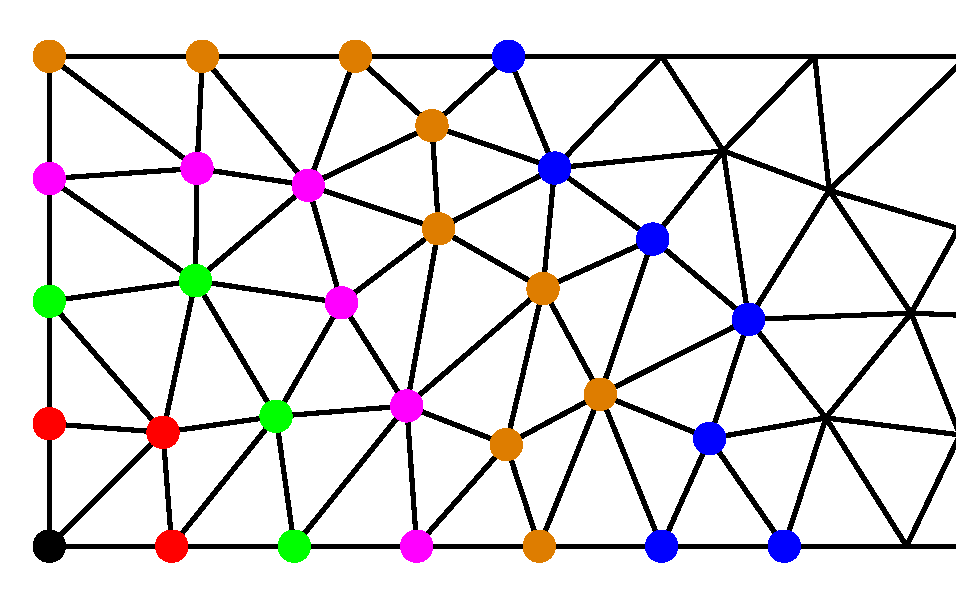
\epsfig{file=wavefronts.eps,height=6cm}
              }
      \caption{Ordering of vertices along spherical wave fronts indicated by different color points. The black point in left-bottom corner is chosen as reference point.}
      \label{fig:wavefronts}
\end{figure}
It is expected that this specific ordering should result in a faster convergence than a random ordering of vertices.

An algorithm is employed that consists of simply proceeding through a list of vertices that remain to be updated. This list is sorted according to the ascending distances
of vertices to the chosen reference point. For a given vertex to be updated,
we first check if its upwave neighbours has already been
updated. If this is the case, this vertex is updated and tagged in the list. Otherwise, the considered vertex is placed untagged and the process continues with the next vertex in the list
of non-updated vertices.
These updates are swept in two cycles. The first cycle involves a forward sweep from the first vertex in the list to the last. The second cycle moves backward from the last to the first.
As such, all directions of characteristics can be covered efficiently.
An iteration is completed when all vertices are updated in both geographic and spectral spaces so that wave energy from all directions has been propagated through geographical space.
This numerical process is iterated until an {\em a priori} convergence condition is satisfied. Here, the curvature-based stopping criteria
as outlined in Section~\ref{sec:stop} will be applied.

\section{Interpolation at user-defined locations}

All the quantities deals with in SWAN are located at the vertices. Hence, due to the user-defined locations of the wave parameters, interpolations are required.
Let parameter $\varphi_j = \varphi(\vec{x}_j)$ and Cartesian coordinates $\vec{x}_j = (x_j, y_j)$, with $j \in \{1,2,3\}$ indicating the vertices of cell $i$, be given.
The vertices 1, 2 and 3 are ordered in a counterclockwise direction, see Figure~\ref{fig:gsunstruc}. The associated 3 edges are denoted as 12, 23 and 31.

Linear interpolation, with $\vec{x}_0$ inside cell $i$ and $\varphi_0 = \varphi(\vec{x}_0)$, is given by
\begin{equation}
  \varphi(\vec{x}) = \varphi_0 + \nabla \varphi \cdot (\vec{x} - \vec{x}_0)
\end{equation}
where $\nabla \varphi$ is a constant vector inside cell $i$. We apply Green-Gauss reconstruction, i.e.,
\begin{equation}
  \nabla \varphi \approx \frac{1}{A_i} \int_{\triangle i} \nabla \varphi d\Omega = \frac{1}{A_i} \oint_{\partial \triangle i}
  \varphi \vec{n} d\Gamma \approx \frac{1}{A_i} \sum_e \varphi_e \vec{n}_e
\end{equation}
where $A_i$ is the area of cell $i$ and the summation runs over the 3 edges $e \in \{12,23,31\}$ of cell $i$.
The values $\varphi_e$ at edges are taken as averages:
\begin{equation}
   \varphi_{12} = \frac{1}{2} (\varphi_1+\varphi_2)\, , \quad
   \varphi_{23} = \frac{1}{2} (\varphi_2+\varphi_3)\, , \quad
   \varphi_{31} = \frac{1}{2} (\varphi_3+\varphi_1)\
\end{equation}
Furthermore, $\vec{n}_e$ is the outward pointing normal
at edge $e$ and is obtained by rotating the edge over 90$^o$ in the clockwise
direction. Hence,
\begin{equation}
  \vec{n}_{12} = R\vec{t}_{12}\, , \quad  R = \left( \begin{array}{ll} 0 & 1 \\ -1 & 0 \end{array} \right) \, , \quad \vec{t}_{12} = \vec{x}_2 - \vec{x}_1
\end{equation}
We also need the following identity
\begin{equation}
   \vec{n}_{12} + \vec{n}_{23} + \vec{n}_{31} = 0
\end{equation}
It is not difficult to show that
\begin{eqnarray}
  \nabla \varphi &=& \frac{1}{2A_i} \left [ \vec{n}_{12} (\varphi_1 - \varphi_3) + \vec{n}_{31} (\varphi_1 - \varphi_2) \right ] \nonumber \\
                 &=& -\frac{1}{2A_i} \left [ \varphi_1 \vec{n}_{23} + \varphi_2 \vec{n}_{31} + \varphi_3 \vec{n}_{12} \right ]
  \label{eq:gradcell}
\end{eqnarray}
or
\begin{equation}
  \frac{\partial \varphi}{\partial x} = \frac{1}{2A_i} \left [ \varphi_1 (y_2 - y_3) + \varphi_2 (y_3 - y_1) + \varphi_3 (y_1 - y_2) \right]
  \label{eq:xgradcell}
\end{equation}
and
\begin{equation}
  \frac{\partial \varphi}{\partial y} = \frac{1}{2A_i} \left [ \varphi_1 (x_3 - x_2) + \varphi_2 (x_1 - x_3) + \varphi_3 (x_2 - x_1) \right]
  \label{eq:ygradcell}
\end{equation}
The area $A_i$ of cell $i$ is given by $|\vec{t}_{12} \cdot \vec{n}_{13}|/2$. Hence, with
\begin{equation}
  \vec{n}_{13} = R\vec{t}_{13} = \left( \begin{array}{l} y_3 - y_1 \\ x_1 - x_3 \end{array} \right)
\end{equation}
we have
\begin{equation}
  A_i = \frac{1}{2} | (x_2 - x_1)(y_3 - y_1) - (x_3 - x_1)(y_2 - y_1) |
\end{equation}
\\[2ex]
\noindent
Alternatively, we may interpolate using the following relation
\begin{equation}
  \varphi(\vec{x}) = \sum_k \varphi_k \lambda_k(\vec{x}) = \varphi_1 \lambda_1 + \varphi_2 \lambda_2 +\varphi_3 \lambda_3
\end{equation}
where $\lambda_k$ is a linear shape function with the following properties:
\begin{enumerate}
  \item $\lambda_k$ is linear per cell and
  \item $\lambda_k(\vec{x}_j) = \delta_{kj}$ with $\delta_{kj}$ is the Kronecker delta.
\end{enumerate}
We choose the following shape function
\begin{equation}
  \lambda_k(\vec{x}) = a_0^k + a_x^k x + a_y^k y
\end{equation}
and the coefficients $a$ follow from solving
\begin{equation}
  \left(
     \begin{array}{lll}
        1 & x_1 & y_1 \\
        1 & x_2 & y_2 \\
        1 & x_3 & y_3
     \end{array}
  \right)
  \left(
     \begin{array}{lll}
        a_0^1 & a_0^2 & a_0^3 \\
        a_x^1 & a_x^2 & a_x^3 \\
        a_y^1 & a_y^2 & a_y^3
     \end{array}
  \right)
  =
  \left(
     \begin{array}{lll}
        1 & 0 & 0 \\
        0 & 1 & 0 \\
        0 & 0 & 1
     \end{array}
  \right)
\end{equation}

\section{Computation of wave-induced force}

{\tt FORCE} is the wave-driven stress, i.e. the force per unit surface driving the wave-driven current, expressed in N/m$^2$, is defined
as the gradient of the radiation stresses:
\begin{equation}
  S_{xx} = \rho g \int \lfloor n \cos^2\theta + n - \frac{1}{2} \rfloor E d\sigma d\theta
\end{equation}
\begin{equation}
  S_{xy} = S_{yx} = \rho g \int n \sin\theta \cos\theta E d\sigma d\theta
\end{equation}
\begin{equation}
  S_{yy} = \rho g \int \lfloor n \sin^2\theta + n - \frac{1}{2} \rfloor E d\sigma d\theta
\end{equation}
with $n$ the ratio of group velocity and phase velocity.
The force is then
\begin{equation}
  F_x = -\frac{\partial S_{xx}}{\partial x} - \frac{\partial S_{xy}}{\partial y}
\end{equation}
and
\begin{equation}
  F_y = -\frac{\partial S_{yx}}{\partial x} - \frac{\partial S_{yy}}{\partial y}
\end{equation}
\\[2ex]
\noindent
In order to compute the force in all internal vertices of the unstructured mesh, we consider a control volume (CV) as depicted in Figure~\ref{fig:cv}.
\begin{figure}[htb]
   \centerline{
      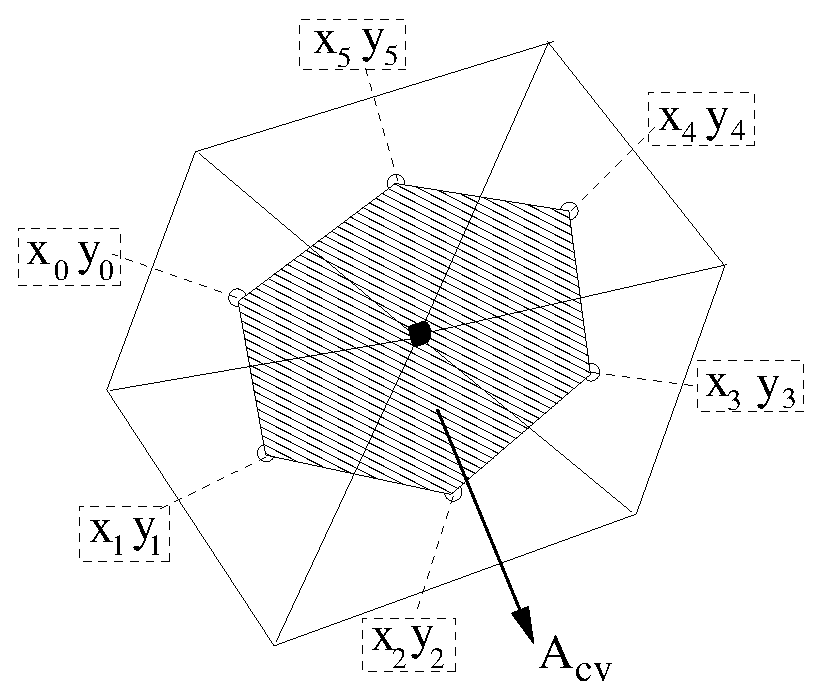
\epsfig{file=CV.eps,height=7cm}
              }
      \caption{Control volume (centroid dual) of vertex is shaded. Some notation is introduced.}
      \label{fig:cv}
\end{figure}
This CV is called centroid dual and is constructed by joining the centroids neighbouring the vertex under consideration. The set of CVs must fill
the whole computational domain and must also be non-overlapping.
In the following we use the numbering from Figure~\ref{fig:cv}.
Let $\varphi$ be one of the
radiation stresses $S_{xx}$, $S_{xy}$ and $S_{yy}$. The gradient of $\varphi$ is computed as follows:
\begin{equation}
  \nabla \varphi \approx \frac{1}{A_{\rm CV}} \sum_e \varphi_e \vec{n}_e
\end{equation}
where $A_{\rm CV}$ is the area of the CV and the summation runs over the associated edges $e$ of this CV.
The values $\varphi_e$ at edges of the centroid dual are taken as averages, i.e. $(\varphi_0+\varphi_1)/2$, $(\varphi_1+\varphi_2)/2$, etc.
Moreover, the value of the radiation stresses
inside each triangle is simply the average of the radiation stresses in the associated vertices of the cell. Now, the derivatives of $\varphi$ inside
CV are
\begin{equation}
  \frac{\partial \varphi}{\partial x} = \frac{1}{2A_{\rm CV}} \sum_{i=0}^{n-1} (\varphi_i+\varphi_{i+1})\,(y_{i+1}-y_i)
  \label{eq:xgradcv}
\end{equation}
and
\begin{equation}
  \frac{\partial \varphi}{\partial y} = \frac{1}{2A_{\rm CV}} \sum_{i=0}^{n-1} (\varphi_i+\varphi_{i+1})\,(x_i-x_{i+1})
  \label{eq:ygradcv}
\end{equation}
with $n$ the number of surrounding cells of the considered vertex and $\varphi_n = \varphi_0$, $x_n = x_0$ and $y_n = y_0$.
The area of the CV is given by
\begin{equation}
  A_{\rm CV} = \frac{1}{2} \sum_{i=0}^{n-1} (x_i\,y_{i+1} - x_{i+1}\,y_i)
\end{equation}

\section{Calculation of diffusion-like terms}

There are situations in which the following diffusion-like term need to be computed on unstructured meshes:
\begin{equation}
  \nabla \cdot \left ( \kappa \nabla \varphi \right )
\end{equation}
in vertices with $\kappa$ a space-varying diffusion coefficient (a tensor) and $\varphi$  a scalar defined in vertices. In SWAN, these are
\begin{itemize}
  \item the alleviation of the garden-sprinkler effect; see Eq. (\ref{eq:gsediff}), and
  \item the computation of the diffraction parameter; see Eq. (\ref{eq3-44}).
\end{itemize}
We consider the centroid dual as shown in Figure~\ref{fig:cv}. The calculation consists of 3 steps. First, we compute the gradient of $\varphi$ inside
each surrounding cell using expressions (\ref{eq:xgradcell}) and (\ref{eq:ygradcell}). Next, this gradient is multiplied with the appropriate diffusion
coefficient $\kappa$ as given in the centroid. Finally, we compute the gradient of $\kappa \nabla \varphi$ inside the CV according to
Eqs. (\ref{eq:xgradcv}) and (\ref{eq:ygradcv}).

\chap{The overall solution algorithm} \label{ch:concl}
This chapter is under preparation.

\newpage
\markboth{}{}
\begin{thebibliography}{10}
\addcontentsline{toc}{chapter}{Bibliography}

\bibitem{Abr92LT}
Abreu, M., A. Larraza and E. Thornton, 1992: Nonlinear transformation of directional wave spectra in
shallow water, {\it J. Geophys. Res}., {\bf 97}, 15579-15589

\bibitem{Alv03B}
Alves, J.H.G.M. and M.L. Banner, 2003: Performance of a saturation-based dissipation-rate source term
in modelling the fetch-limited evolution of wind waves, {\it J. Phys. Oceanogr}., {\bf 33}, 1274-1298

\bibitem{Arc90L}
Arcilla, A.S. and C.M. Lemos, 1990: {\it Surf-Zone Hydrodynamics}, Centro Internacional de M\'{e}todos
Num\'{e}ricos en Ingenieria, Barcelona, 310 p.

\bibitem{Arc94RC}
Arcilla, A.S., J.A. Roelvink, B.A. O'Connor, A.J.H.M. Reniers and J.A. Jimenez, 1994: The Delta flume '93
experiment, {\it Proc. Coastal Dynamics Conf. '94}, 488-502

\bibitem{Ban94Y}
Banner, M.L. and I.R. Young, 1994: Modelling spectral dissipation in the evolution of wind waves. Part I:
Assessment of existing model performance, {\it J. Phys. Oceanogr}., {\bf 24}, No. 7, 1550-1571

\bibitem{Templates94}
R.~Barrett, M.~Berry, T.F.~Chan, J.~Demmel, J.~Donato, J.~Dongarra, V.~Eijkhout,
  R.~Pozo, C.~Romine, H.~van~der Vorst, Templates for the solution of linear
  systems: {B}uilding blocks for iterative methods, SIAM, Philadelphia, PA,
  1994, accessible from \hl{http://www.netlib.org/templates/Templates.html}.

\bibitem{Bas91H}
P.~Bastian, G.~Horton, Parallelization of robust multi-grid methods: {ILU}
  factorization and frequency decomposition method, SIAM J. Sci. Stat. Comput.
  12 (1991) 1457--1470.

\bibitem{Bat78J}
Battjes, J.A. and J.P.F.M. Janssen, 1978: Energy loss and set-up due to breaking of random waves, {\it Proc.
16$^{{\rm th}}$ Int. Conf. Coastal Engineering}, ASCE, 569-587

\bibitem{Bat84V}
Battjes, J.A. and G.Ph. van Vledder, 1984, Verification of Kimura's theory for wave group statistics, {\it Proc.
19$^{{\rm th}}$ Int. Conf. Coastal Engineering}, ASCE, Houston, 642-648

\bibitem{Bat85S}
Battjes, J.A. and M.J.F. Stive, 1985: Calibration and verification of a dissipation model for random breaking
waves, {\it J. Geophys. Res}., {\bf 90}, No. C5, 9159-9167

\bibitem{Bat92B}
Battjes, J.A. and S. Beji, 1992: Breaking waves propagating over a shoal, {\it Proc. 23$^{{\rm rd}}$ Int. Conf. Coastal
Engineering}, ASCE, 42-50

\bibitem{Bat94}
Battjes, J.A., 1994: Shallow water wave modelling, M. Isaacson and M. Quick (Eds.), {\it Proc. Waves-Physical
and Numerical Modelling}, University of British Columbia, Vancouver, 1-24

\bibitem{Bej93B}
Beji, S. and J.A. Battjes 1993: Experimental investigation of wave propagation over a bar, {\it Coastal
Engineering}, {\bf 19}, 151-162

\bibitem{Ben96}
Bender, L.C., 1996, Modification of the physics and numerics in a third-generation ocean wave model, {\it J.
Atm. and Ocean. Techn}., 13, 3, 726-750

\bibitem{Bid96HJ}
Bidlot, J.-R., B. Hansen and P.A.E.M. Janssen, 1996: Wave modelling and operational forecasting at
ECMWF, {\it 1$^{{\rm st}}$ International Conference on EuroGOOS}, 7-11 October, 1996, The Hague, 206-213

\bibitem{Ben96MB}
Benoit, M., F. Marcos and F. Becq, 1996: Development of a third-generation shallow-water wave model
with unstructured spatial meshing. {\it Proc. 25$^{{\rm th}}$ Int. Conf. Coastal Engineering}, ASCE, Orlando,
465-478

\bibitem{Ben05}
Benoit, M., 2005: Evaluation of methods to compute the non-linear quadruplet interactions for deep-water wave spectra,
{\it Proc. 5th Int. Symp. WAVES 2005}, Madrid, Spain

\bibitem{Ber72}
Berkhoff, J.C.W., 1972: Computation of combined refraction-diffraction, {\it Proc. 13$^{{\rm th}}$ Int. Conf. Coastal
Engineering}, ASCE, 471-490

\bibitem{Ber94C}
Bertotti, L and L. Cavaleri, 1994: Accuracy of wind and wave evaluation in coastal regions, {\it Proc. 24$^{{\rm th}}$ Int.
Conf. Coastal Engineering}, ASCE, 57-67

\bibitem{Bil03S}
Bilgili, A. and Smith, K.W., 2003.
BatTri: a 2-D finite element grid generator, version 11.11.03.
Available from: \hl{http://www-nml.dartmouth.edu/Publications/internal\_reports/NML-03-15/}.

\bibitem{Boo87H}
Booij, N., and L.H. Holthuijsen, 1987, Propagation of ocean waves in discrete spectral wave m{\it odels,
Journal of Computational Physics}, vol. 68, 307-326.

\bibitem{Boo92HL}
Booij, N., L.H. Holthuijsen and P.H.M. de Lange, 1992, The penetration of short-crested waves through
a gap, {\it Proc. 23rd Int. Conf. Coastal Eng}, Venice 4-9 Oct., 1992, New York, 1993, 1044-1052

\bibitem{Boo96HR}
Booij, N., L.H. Holthuijsen and R.C. Ris, 1996: The "SWAN" wave model for shallow water, {\it Proc. 25th Int.
Conf. Coastal Engng.}, Orlando, 668-676

\bibitem{Boo97HPa}
Booij, N., L.H. Holthuijsen and R. Padilla-Hernandez, 1997: A nonstationary, parametric coastal wave
model, {\it Conf. Coastal Dynamics '97}, Plymouth, 99-107

\bibitem{Boo97HPb}
Booij, N., L.H. Holthuijsen and R. Padilla-Hernandez, 1997: Numerical wave propagation on a curvi-linear
grid, {\it Proceedings 3rd International Symposium on Ocean Wave Measurement and Analysis, WAVES '97}, ASCE, 286-294

\bibitem{Boo98HR}
Booij, N., L.H. Holthuijsen and R.C. Ris, 1998: Shallow water wave modelling, {\it Oceanology International
98, The Global Ocean, Brighton, Conference Proceedings}, 3, 483-491

\bibitem{Boo98HH}
Booij, N., L.H. Holthuijsen and IJ.G. Haagsma, 1998: Comparing the second-generation HISWA wave
model with the third-generation SWAN wave model, {\it 5th International Workshop on Wave
Hindcasting and Forecasting}, Melbourne, Florida, 215-222

\bibitem{Boo99RH}
Booij, N., R.C. Ris and L.H. Holthuijsen, 1999, A third-generation wave model for coastal regions, Part I,
Model description and validation, {\it J.Geoph.Research}, 104, C4, 7649-7666

\bibitem{Boo01HB}
Booij, N., L.H. Holthuijsen and J.A. Battjes, 2001: Ocean to near-shore wave modelling with SWAN,
{\it 4th International Conference on Coastal Dynamics 2001}, Lund, Sweden, 335-344

\bibitem{Boo01HH}
Booij, N., L.H. Holthuijsen and IJ.G. Haagsma, 2001: The effect of swell on the generation and dissipation
of waves, {\it 4th International Symposium on Ocean Wave Measurements and Analysis WAVES 2001},
San Francisco, 501-506

\bibitem{Bot85E}
Botta, E.F.F. and M.H.M. Ellenbroek, 1985: A modified SOR method for the Poisson equation in unsteady free-surface
flow calculations, {\it J. Comput. Phys.}, {\bf 60}, 119-134

\bibitem{Bou82B}
Bouws, E. and J.A. Battjes, 1982: A Monte-Carlo approach to the computation of refraction  of water waves,
{\it J. Geophys. Res}., {\bf 87}, 5718-5722

\bibitem{Bou83K}
Bouws, E. and G.J. Komen, 1983: On the balance between growth and dissipation in an extreme, depth-limited
wind-sea in the southern North Sea, {\it J. Phys. Oceanogr}., {\bf 13}, 1653$-$1658

\bibitem{Cam02CR}
Campbell, T., J.~Cazes, E.~Rogers, Implementation of an important wave model on
  parallel architectures, in: Oceans 2002 MTS/IEEE Conference, IEEE, 2002, pp.
  1509--1514, available from
  \hl{http://www7320.nrlssc.navy.mil/mts2002/PDF/campbell-paper.pdf}.

\bibitem{Car76PW}
Cardone, V.J., W.J. Pierson and E.G. Ward, 1976: Hindcasting the directional spectra of hurricane-generated waves,
{\it J. Petr. Techn}., {\bf 28}, 385-394

\bibitem{Cav81M}
Cavaleri, L. and P. Malanotte-Rizzoli, 1981: Wind wave prediction in shallow water: Theory and
applications. {\it J. Geophys. Res}., {\bf 86}, No. C11, 10,961-10,973

\bibitem{Cav98H}
Cavaleri, L. and L.H. Holthuijsen, 1998: Wave modelling in the WISE group, {\it Proc. 26th Int. Conf. Coastal
Engng}., Copenhagen, 498-508

\bibitem{CER73}
CERC, 1973: Shore Protection Manual, U.S. Army Corps of Engineers, Techn. Rep. No. 4, Vol. I

\bibitem{Che83W}
Chen, Y. and H. Wang, 1983: Numerical model for nonstationary shallow water wave spectral
transformations, {\it J. Geophys. Res}., {\bf 88}, 9851-9863

\bibitem{Che97GE}
Chen, Y., R.T. Guza, and S. Elgar, 1997: Modelling of breaking surface waves in shallow water, {\it J. Geophys. Res}.,
102, C11, 25035-25046

\bibitem{Chr94HR}
Chrisochoides, N.P., E.N.~Houstis, J.R.~Rice, Mapping algorithms and software
  environment for data parallel {PDE} iterative solvers, J. Parallel and Distr.
  Comput. 21 (1994) 75--95.

\bibitem{Col72}
Collins, J.I., 1972: Prediction of shallow water spectra, {\it J. Geophys. Res}., {\bf 77}, No. 15, 2693-2707

\bibitem{Dal84KH}
Dalrymple, R.A., J.T. Kirby and P.A. Hwang, 1984: Wave diffraction due to areas of energy dissipation,
{\it Journal of Waterways, Ports, Harbours and Coastal Engineering}, {\bf 110}, 67-79

\bibitem{Dan96MJ}
d'Angremond, K., J.W.~van der Meer and R.J. de Jong, 1996: Wave transmission at low-crested structures,
{\it Proc. 25$^{{\rm th}}$ Int. Conf. Coastal Engng.}, ASCE, Orlando, 2418-2427

\bibitem{Din78RV}
Dingemans, M.W., A.C. Radder and H.J. de Vriend, 1978: Computations of the driving forces of wave-induced
currents, {\it Coastal Engng}., 11, 539-563

\bibitem{DeW01}
{De Waal}, J.P., 2001. Wave growth limit in shallow water. Proc. 4th Int. Symp. Waves 2001, pp. 560--569.

\bibitem{Din97}
Dingemans, M.W., 1997: Water wave propagation over uneven bottoms. Part 1 -linear wave propagation,
{\it Advanced Series on Ocean Engineering}, 13, World Scientific, 471 p.

\bibitem{Eld96}
Eldeberky, Y., 1996: Nonlinear transformation of wave spectra in the nearshore zone, {\it Ph.D. thesis}, Delft
University of Technology, Department of Civil Engineering, The Netherlands

\bibitem{Eld95B}
Eldeberky, Y. and J.A. Battjes, 1995: Parameterization of triad interactions in wave energy models, {\it Proc.
Coastal Dynamics Conf. '95}, Gdansk, Poland, 140-148

\bibitem{Eld96B}
Eldeberky, Y. and J.A. Battjes, 1996: Spectral modelling of wave breaking: Application to Boussinesq
equations, {\it J. Geophys. Res}., {\bf 101}, No. C1, 1253-1264

\bibitem{ELg86G}
Elgar, S. and R.T. Guza, 1986: Nonlinear model predictions of bispectra of shoaling surface gravity waves,
{\it J. Fluid Mech.}, 167, 1-18

\bibitem{Elg97GRHG}
Elgar, S., R.T. Guza, B. Raubenheimer, T.H.C. Herbers and E.L. Gallagher, 1997: Spectral evolution of
shoaling and breaking waves on a barred beach, {\it J. Geophys. Res}., 102,C7, 15797-15805

\bibitem{Ewi71}
Ewing, J.A., 1971: A numerical wave prediction method for the North Atlantic Ocean, {\it Deutsch. Hydrogr. Z}.,
{\bf 24}, No. 6, 241$-$261

\bibitem{Ewi93H}
Ewing, J.A. and R.C. Hague, 1993: A second-generation wave model for coastal wave prediction, {\it Proc.
of 2$^{{\rm nd}}$ Int. Symposium on Ocean Wave Measurement and Analysis}, New Orleans, 576-589

\bibitem{Fle88}
Fletcher, C.A.J., 1988: {\it Computational Techniques for Fluid Dynamics, Parts I and II,} Springer, 409+484
p.

\bibitem{Fer99P}
Ferziger, J.H. and Peri\'{c}, M., 1999. Computational methods for fluid dynamics (2nd edition).
  Springer-Verlag, Berlin.

\bibitem{Fox88}
G.C.~Fox, A review of automatic load balancing and decomposition methods for the
  hypercube, in: M.~Schulz (Ed.), Numerical Algorithms for Modern Parallel
  Computer Architectures, Springer, Verlag, 1988, pp. 63--76, IMA volume 13.

\bibitem{Fre84G}
Freilich, M.H. and R.T. Guza, 1984: nonlinear effects on shoaling surface gravity waves, {\it Phil. Trans. R.
Soc. London, }A 311, 1-41

\bibitem{Gal72}
Galvin, C.J., 1972: Wave breaking in shallow water, {\it Waves on beaches and resulting sediment transport},
Academic Press Inc., 413-455

\bibitem{Gel56CV}
Gelci, R., H. Cazal\'{e} and J. Vassal, 1956: Utilization des diagrammes de propagation \`{a} la pr\'{e}vision
\'{e}nerg\'{e}tique de la houle, {\it Bulletin d'information du Comit\'{e} Central d'oc\'{e}anographie et d'\'{e}tudes
des c\^{o}tes}, {\bf 8}, No. 4, 160-197 (in French)

\bibitem{God67TM}
Goda, Y., H. Takeda and Y. Moriya, 1967: Laboratory investigation of wave transmission over breakwaters{\it ,
Rep. port and Harbour Res. Inst}., 13 (from Seelig, 1979)

\bibitem{Gol83}
Golding, B.W., 1983: A wave prediction system for real-time sea state forecasting, {\it J. R. Met. Soc}., {\bf 109},
393-416

\bibitem{Gol86L}
Golub, G.H. and C.F. van Loan, 1986: Matrix Computations, North Oxford Academic, London, 476 p.

\bibitem{Gor99N}
Gorman, R.M. and C.G. Neilson, 1999: Modelling shallow water wave generation and transformation in
an intertidal estuary, {\it Coastal Engineering}, 36, 197-217

\bibitem{Gro99LS}
W.~Gropp, E.~Lusk, A.~Skjellum, Using {MPI}: {P}ortable parallel programming
  with the {M}essing {P}assing {I}nterface, MIT Press, Cambridge, MA, 1999.

\bibitem{Gun92HJ}
G\"{u}nther, H., S. Hasselmann and P.A.E.M. Janssen, 1992: The WAM model Cycle 4 (revised version),
{\it Deutsch. Klim. Rechenzentrum, Techn. Rep. No. 4}, Hamburg, Germany

\bibitem{Har01A}
Hargreaves, J.C. and Annan, J.D., 2001. Comments on ``{I}mprovement of the short-fetch behavior
  in the wave ocean model ({WAM})''. J. Atmos. Oceanic Techn., 18: 711--715.

\bibitem{Has02HH}
Hashimoto, N., IJ.G. Haagsma and L.H. Holthuijsen, 2002: Four-wave interactions in SWAN, {\it Proc. 28$^{{\rm th}}$
Int. Conf. Coastal Engng.}, ASCE, Cardiff, 392-404

\bibitem{Has60}
Hasselmann, K., 1960: Grundgleichungen der Seegangsvoraussage, {\it Schiffstechnik}, 1,  191$-$195

\bibitem{Has62}
Hasselmann, K., 1962: On the non-linear transfer in a gravity wave spectrum, part 1. {G}eneral theory,
{\it J. Fluid Mech.}, {\bf 12}, 481-500

\bibitem{Has63a}
Hasselmann, K., 1963a: On the non-linear transfer in a gravity wave spectrum, part 2. {C}onservation theory,
wave-particle correspondence, irreversibility,
{\it J. Fluid Mech.}, {\bf 15}, 273-281

\bibitem{Has63b}
Hasselmann, K., 1963b: On the non-linear transfer in a gravity wave spectrum, part 3. {E}valuation of energy
flux and sea-swell interactions for a {N}euman spectrum,
{\it J. Fluid Mech.}, {\bf 15}, 385-398

\bibitem{Has68C}
Hasselmann, K. and J.I. Collins, 1968: Spectral dissipation of finite-depth gravity waves due to turbulent
bottom friction, {\it J. Mar. Res}., {\bf 26}, 1-12

\bibitem{JON73}
Hasselmann, K., T.P. Barnett, E. Bouws, H. Carlson, D.E. Cartwright, K. Enke, J.A. Ewing, H. Gienapp,
D.E. Hasselmann, P. Kruseman, A. Meerburg, P. M\"{u}ller, D.J. Olbers, K. Richter, W. Sell and H.
Walden, 1973: Measurements of wind$-$wave growth and swell decay during the Joint North Sea
Wave Project (JONSWAP), {\it Dtsch. Hydrogr. Z}. Suppl., {\bf 12}, A8

\bibitem{Has74}
Hasselmann, K., 1974: On the spectral dissipation of ocean waves due to whitecapping, {\it Bound.-layer
Meteor}., {\bf 6}, 1-2, 107-127

\bibitem{Has76RMS}
Hasselmann, K., D.B. Ross, P. M\"{u}ller and W. Sell, 1976: A parametric wave prediction  model, {\it J. Phys.
Oceanogr.}, {\bf 6}, 200$-$228

\bibitem{Has81H}
Hasselmann, S. and K. Hasselmann, 1981: A symmetrical method of computing the non-linear transfer
in a gravity-wave spectrum, {\it Hamburger Geophys. Einzelschr}., Serie A., 52, 8

\bibitem{Has85HAB}
Hasselmann, S., K. Hasselmann, J.H. Allender and T.P. Barnett, 1985: Computations and
parameterizations of the nonlinear energy transfer in a gravity wave spectrum. Part II:
Parameterizations of the nonlinear transfer for application in wave models, {\it J. Phys. Oceanogr}.,
{\bf 15}, 11, 1378-1391

\bibitem{Hed87}
Hedges, T.S., 1987: Combination of waves and currents: an introduction, {\it Proc. Instn. Civ. Engrs}., Part 1,
{\bf 82}, 567-585

\bibitem{Her99J}
Hersbach, H. and Janssen, P.A.E.M., 1999. Improvement of the short-fetch behavior in the wave ocean
model ({WAM}). J. Atmos. Oceanic Techn., 16: 884--892.

\bibitem{Her80H}
Herterich, K. and K. Hasselmann, 1980: A similarity relation for the nonlinear energy transfer in a
finite-depth gravity-wave spectrum, {\it J. Fluid Mech.}, {\bf 97}, 215-224

\bibitem{Hol80}
Holthuijsen, L.H., 1980: Methods of wave prediction, part I and II (Methoden voor golfvoorspelling, deel I
en II, in Dutch), Technical Advisory Commission against Inundation (Technische
Adviescommissie voor de Waterkeringen, in Dutch), Den Haag, The Netherlands

\bibitem{Hol88B}
Holthuijsen, L.H. and S. De Boer, 1988: Wave forecasting for moving and stationary targets, {\it Computer
modelling in Ocean Engineering}, Eds. B.Y. Schrefler and O.C. Zienkiewicz, Balkema, Rotterdam,
The Netherlands, 231-234

\bibitem{Hol89BH}
Holthuijsen, L.H., Booij, N. and T.H.C. Herbers, 1989: A prediction model for stationary, short-crested
waves in shallow water with ambient currents, {\it Coastal Engineering}, {\bf 13}, 23-54

\bibitem{Hol93BR}
Holthuijsen, L.H., N. Booij and R.C. Ris, 1993: A spectral wave model for the coastal zone, {\it Proceedings
2nd International Symposium on Ocean Wave Measurement and Analysis}, New Orleans,
Louisiana, July 25$-$28, 1993: New York, pp. 630$-$641

\bibitem{Hol96BB}
Holthuijsen, L.H., N. Booij and L. Bertotti, 1996: The propagation of wind errors through
ocean wave hindcasts, {\it J. Offshore Mech. And Arctic Eng.}, {\bf 118}, 184-189

\bibitem{Hol97BP}
Holthuijsen, L.H., N. Booij and R. Padilla-Hernandez, 1997: A curvi-linear, third-generation coastal wave
model, {\it Conf. Coastal Dynamics '97}, Plymouth, 128-136

\bibitem{Hol97BRAJ}
Holthuijsen, L.H., N. Booij, R. Ris, J.H. Andorka Gal and J.C.M. de Jong, 1997: A verification of the third-generation
wave model "SWAN" along the southern North Sea coast,  {\it Proceedings 3rd
International Symposium on Ocean Wave Measurement and Analysis, WAVES '97}, ASCE, 49-63

\bibitem{Hol98a}
Holthuijsen, L.H., 1998: The concept and features of the ocean wave spectrum,
Provision and engineering/operational application of ocean wave spectra,
{\it COST Conference}, UNESCO, 21-25 sept., Paris, keynote address, 11-20

\bibitem{Hol98b}
Holthuijsen, L.H., 1998: Waves in shallow water,
{\it World Meteorological Organization Guide to wave analysis and forecasting},
WMO-N0. 702, Chapter 7, 81-88

\bibitem{Hol98RB}
Holthuijsen, L.H., R.C. Ris and N. Booij, 1998: A verification of the third-generation wave model SWAN,
{\it 5th International Workshop on Wave Hindcasting and Forecasting}, Melbourne, Florida, 223-230

\bibitem{Hol98BH}
Holthuijsen, L.H., N. Booij and IJ.G. Haagsma, 1998: Comparing 1$^{{\rm st}}$-, 2$^{{\rm nd}}$ - and 3$^{{\rm rd}}$-generation
coastal wave modelling,  {\it 26th Int. Conf. Coastal Engng}., Copenhagen, 140-149

\bibitem{Hol00B}
Holthuijsen, L.H. and N. Booij, 2000: Oceanic and near-shore whitecapping effects in SWAN, 6$^{{\rm th}}$ Int.
Workshop on Wave Hindcasting and Forecasting, Monterey, 362-368

\bibitem{Hol00RBC}
Holthuijsen, L.H, R.C. Ris, N. Booij and E.Cecchi, 2000: Swell and whitecapping, a numerical experiment,
{\t Proc. 27th Int. Conf. Coastal Engng.}, Sydney, 346-354

\bibitem{Hol03HB}
Holthuijsen, L.H., Herman, A. and Booij, N., 2003: Phase-decoupled refraction-diffraction for
spectral wave models, {\it Coastal Engineering}, {\bf 49}, 291-305

\bibitem{Hol07}
Holthuijsen, L.H., 2007: {\it Waves in oceanic and coastal waters},
Cambridge University Press.

\bibitem{Hsu05OL}
Hsu, T.-W., S.-H. Ou and J.-M. Liau, 2005: Hindcasting nearshore wind waves using a FEM code for SWAN,
{\it Coastal Engineering}, {\bf 52}, 177-195

\bibitem{Jan89}
Janssen, P.A.E.M., 1989: Wave induced stress and the drag of air flow over sea waves, {\it J. Phys.
Oceanogr}., {\bf 19}, 745-754

\bibitem{Jan91a}
Janssen, P.A.E.M., 1991a: Quasi-linear theory of wind-wave generation applied to wave forecasting, {\it J.
Phys. Oceanogr}., {\bf 21}, 1631-1642

\bibitem{Jan91b}
Janssen, P.A.E.M., 1991b: Consequences of the effect of surface gravity waves on the mean air flow, {\it Int.
Union of Theor. and Appl. Mech}. (IUTAM), Sydney, Australia, 193-198

\bibitem{Jon66}
Jonsson, I.G. 1966: Wave boundary layers and friction factors, {\it Proc. 10$^{{\rm th}}$ Int. Conf. Coastal Engineering},
ASCE, 127-148

\bibitem{Jon80}
Jonsson, I.G., 1980: A new approach to rough turbulent boundary layers, {\it Ocean Engineering}, {\bf 7}, 109-152

\bibitem{Jon93}
Jonsson, I.G., 1993: {\it The Sea}, Ocean Engineering Science, {\bf 9}, Part A

\bibitem{Jon76C}
Jonsson, I.G. and N.A. Carlsen, 1976: Experimental and theoretical investigations in an oscillatory
turbulent boundary layer, {\it J. Hydraulic Research}, {\bf 14}, 45-60

\bibitem{Kah92C}
Kahma, K.K. and C.J. Calkoen, 1992: Reconciling discrepancies in the observed growth of
wind$-$generated waves, {\it J. Phys. Oceanogr}., {\bf 22}, 1389$-$1405

\bibitem{Kam93K}
Kaminsky, G.M. and N.C. Kraus, 1993: Evaluation of depth-limited wave breaking criteria, {\it Proc.
of 2$^{{\rm nd}}$ Int. Symposium on Ocean Wave Measurement and Analysis}, New Orleans, 180-193

\bibitem{Kar69}
Karlson, T, 1969: Refraction of continuous ocean wave spectra, {\it Journal of Waterways, Ports, Harbours
and Coastal Engineering}, {\bf 95}, 275-287

\bibitem{Kir86}
Kirby, J.T., 1986: Higher-order approximation in the parabolic equation method for water waves, {\it J.
Geophys. Res.}, {\bf 91}, C1, 933-952

\bibitem{Kom84HH}
Komen, G.J., S. Hasselmann, and K. Hasselmann, 1984: On the existence of a fully developed wind-sea
spectrum, {\it J. Phys. Oceanogr}., {\bf 14}, 1271-1285

\bibitem{Kom94CDHHJ}
Komen, G.J., Cavaleri, L., Donelan, M., Hasselmann, K., Hasselmann, S. and P.A.E.M. Janssen, 1994:
{\it Dynamics and Modelling of Ocean Waves}, Cambridge University Press, 532 p.

\bibitem{Kui88VH}
Kuik, A.J., G.Ph. van Vledder and L.H. Holthuijsen, 1988: A method for the routine  analysis of
pitch-and-roll buoy wave data, {\it J. Phys. Oceanogr}., {\bf 18}, 1020-1034

\bibitem{Li92M}
Li, C.W. and M. Mao, 1992: Spectral modelling of typhoon-generated waves in shallow waters, {\it J.
Hydraulic Research}, {\bf 30}, 5, 611-622

\bibitem{Lin96H}
Lin, R.Q. and N.E. Huang, 1996: the Goddard coastal wave model. Part I: Numerical method, {\it J. Phys.
Oceanogr}., {\bf 26}, 833-847

\bibitem{Liu85YK}
Liu, P.L., S.B. Yoon and J.T. Kirby, 1985: Nonlinear refraction-diffraction of waves in shallow water, {\it J. Fluid
Mech.}, 153, 185-201

\bibitem{Luo94M}
Luo, W. and J. Monbaliu, 1994: Effects of the bottom friction formulation on the energy balance for gravity
waves in shallow water, {\it J. Geophys. Res}., {\bf 99}, C9, 18,501-18,511

\bibitem{Mad88PG}
Madsen, O.S., Y.-K. Poon and H.C. Graber, 1988: Spectral wave attenuation by bottom friction: Theory,
{\it Proc. 21$^{{\rm th}}$ Int. Conf. Coastal Engineering}, ASCE, 492-504

\bibitem{Mad92S}
Madsen, P.A. and O.R. S{\o}rensen, 1992: A new form of the Boussinesq equations with improved linear
dispersion characteristics. Part 2: A slowly-varying bathymetry, {\it Coastal Engineering}, {\bf 18}, 183-205

\bibitem{Mad93S}
Madsen, P.A. and O.R. S{\o}rensen, 1993: Bound waves and triad interactions in shallow water, {\it Ocean
Engineering,} {\bf 20}, 4, 359-388

\bibitem{Mas92K}
Mase, H. and J.T. Kirby, 1992: Hybrid frequency-domain KdV equation for random wave transformation,
{\it Proc. 23$^{{\rm th}}$ Int. Conf. Coastal Engineering}, ASCE, 474-487

\bibitem{Mas93BJ}
Mastenbroek, C., G. Burgers, and P.A.E.M. Janssen, 1993: The dynamical coupling of a wave model in
a storm surge model through the atmospheric boundary layer, {\it J. Phys. Oceanogr}., {\bf 23}, 1856-1866

\bibitem{Mee05BZW}
Van der Meer, J.W., R. Briganti, B. Zanuttigh and B. Wang, 2005: Wave transmission and reflection at
low-crested structures: design formulae, oblique wave attack and spectral change,
{\it Coast. Engng}., {\bf 52}, 915-929

\bibitem{Men04L}
Mendez, F.J. and I.J. Losada, 2004: An empirical model to estimate the propagation of random breaking and
nonbreaking waves over vegeation fields, {\it Coast. Engng}., {\bf 51}, 103-118

\bibitem{Mei83}
Mei, C.C., 1983: {\it The applied dynamics of ocean surface waves}, Wiley, New York, 740 p.

\bibitem{Meu88}
G.~Meurant, Domain decomposition methods for partial-differential equations on
  parallel computers, Int. J. Supercomputer Appl. and High Perform. Comput. 2
  (4) (1988) 5--12.

\bibitem{Mil57}
Miles, J.W., 1957: On the generation of surface waves by shear flows, {\it J. Fluid Mech}., {\bf 3}, 185$-$204

\bibitem{Mil81}
Miles, J.W., 1981: Hamiltonian formulations for surface waves, {\it Applied Scientific Research}, {\bf 37}, 103-110

\bibitem{Nel87}
Nelson, R.C., 1987: Design wave heights on very mild slopes: An experimental study, {\it Civil. Eng. Trans.,
Inst. Eng. Aust}., {\bf 29}, 157-161

\bibitem{Nel94}
Nelson, R.C., 1994: Depth limited design wave heights in very flat regions, {\it Coastal Engineering}, {\bf 23}, 43-59

\bibitem{Nel97}
Nelson, R.C., 1997: Height limits in top down and bottom up wave environments, {\it Coastal Engineering},
{\bf 32}, 247-254

\bibitem{Nwo94}
Nwogu, O., 1994: Nonlinear evolution of directional wave spectra in shallow water, {\it Proc. 24$^{{\rm th}}$ Int. Conf.
Coastal Engineering}, ASCE, 467-481

\bibitem{Omp}
OpenMP~ARB, {OpenMP}, \hl{http://www.openmp.org}.

\bibitem{Pad98OMH}
Padilla-Hernandez, R., P. Osuna, J. Monbaliu and L. Holthuijsen, 1998: Intercomparing third-generation
wave model nesting, {\it 5th International Workshop on Wave Hindcasting and Forecasting}, Melbourne, Florida, 102-112

\bibitem{Per66}
Peregrine, D.H., 1966: Long waves on a beach, {\it J. Fluid Mech}., {\bf 27}, 4, 815-827

\bibitem{Phi57}
Phillips, O.M., 1957: On the generation of waves by turbulent wind, {\it J. Fluid Mech}., {\bf 2}, 417$-$445

\bibitem{Phi60}
Phillips, O.M., 1960: On the dynamics of unsteady gravity waves of finite amplitude. Part 1, {\it J. Fluid Mech}.,
{\bf 9}, 193-217

\bibitem{Phi77}
Phillips, O.M., 1977: {\it The dynamics of the upper ocean}, Cambridge University Press, 336 p.

\bibitem{Phi85}
Phillips, O.M., 1985: Spectral and statistical properties of the equilibrium range in wind-generated gravity
waves, {\it J. Fluid Mech}., {\bf 156}, 505-531

\bibitem{Pie64M}
Pierson, W.J. and L. Moskowitz, 1964: A proposed spectral form for fully developed wind seas based on
the similarity theory of S.A. Kitaigorodskii, {\it J. Geophys. Res}., {\bf 69}, 24, 5181-5190

\bibitem{Pie65}
Piest, J., 1965: Seegangsbestimmung und Seegangsrefraktion in einem Meer mit nicht- ebenem Boden;
eine theoretische Untersuchung, {\it Deutsch. Hydrogr. Z}., {\bf 18}: 67-74 (in German)

\bibitem{Pre93FTV}
Press, W.H., Flannery, B.P., Teukolsky, S.A. and Vetterling, W.T., 1993. Numerical recipes in Fortran~77.
The art of scientific computing (2nd edition). Cambridge University Press, New York (available from
\hl{http://www.nr.com}).

\bibitem{Put49J}
Putnam, J.A. and J.W. Johnson, 1949: The dissipation of wave energy by bottom friction, {\it Trans. Am.
Geoph. Union}, {\bf 30}, 67-74

\bibitem{Rad79}
Radder, A.C., 1979: On the parabolic equation method for water-wave propagation, {\it J. Fluid Mech}., {\bf 95},
159-176

\bibitem{Rad92}
Radder, A.C., 1992: An explicit Hamiltonian formulation of surface waves in water of finite depth, {\it J. Fluid
Mech.}, {\bf 237}, 435-455

\bibitem{Rad96}
Radder, A.C., 1996: Hamiltonian dynamics of water waves, {\it Advances of Coastal and Ocean Engineering},
World Scientific, {\bf 4}, ??-??

\bibitem{Res91P}
Resio, D. and W. Perrie, 1991: A numerical study of nonlinear energy fluxes due to wave-wave
interactions. Part I: Methodology and basic results, {\it J. Fluid Mech}., {\bf 223}, 609-629

\bibitem{Res01PTV}
Resio, D.T., J.H. Pihl, B.A. Tracy and C.L. Vincent, 2001: Nonlinear energy fluxes and  the finite depth equilibrium
range wave spectra, {\it J. Geophys. Res.}, {\bf 106}, C4, 6985-7000.

\bibitem{Res04LV}
Resio, D.T., C.E. Long and C.L. Vincent, 2004: Equilibrium-range constant in wind-generated wave spectra,
{\it J. Geophys. Res.}, {\bf 109}, C01018.

\bibitem{Ris94HB}
Ris, R.C., L.H. Holthuijsen and N. Booij, 1994: A spectral model for waves in the near shore zone, {\it Proc.
24th Int. Conf. Coastal Engng}, Kobe, Japan, pp. 68-78

\bibitem{Ris96H}
Ris, R.C. and L.H. Holthuijsen, 1996: Spectral modelling of current wave-blocking.
{\it Proc. 25$^{{\rm th}}$ Int. Conf. Coastal Engng.}, ASCE, 1247-1254.

\bibitem{Ris97H}
Ris, R.C. and L.H. Holthuijsen, 1997: Modelling of current induced wave-blocking in a spectral wave
model, {\it 8$^{{\rm th}}$ International Biennal Conference on  Physics of Estuaries and Coastal Seas}, J.
Dronkers and M.B.A.M. Scheffers (eds.), The Hague, 139-144

\bibitem{Ris99}
Ris, R.C., 1999. Model convergence of SWAN in the Westerschelde estuary.
WL$\vert$Delft Hydraulics, Report H3496.

\bibitem{Ris99BH}
Ris, R.C., N. Booij and L.H. Holthuijsen, 1999: A third-generation wave model for coastal regions, Part II:
Verification,  {\it J. Geophys. Res}., 104, C4, 7667-7681

\bibitem{Ris02HSBD}
Ris, R., L.H. Holthuijsen, J.M. Smith, N. Booij and A.R. van Dongeren, 2002: The ONR virtual testbed
for coastal and oceanic wave models, {\it Proc. 28$^{{\rm th}}$ Int. Conf. Coastal Engng.}, ASCE, Cardiff, 380-391

\bibitem{Roa72}
Roache, P.J., 1972: {\it Computational Fluid Dynamics}, Hermosa Publishers, Albuquerque, 446 p.

\bibitem{Rog02KPBH}
Rogers, W.E., J.M. Kaihatu, H.A. H. Petit, N. Booij, and L.H. Holthuijsen, 2002: Diffusion reduction in a
arbitrary scale third generation wind wave model, {\it Ocean Engng}., {\bf 29}, 1357-1390.

\bibitem{Rog03HW}
Rogers, W.E., P.A. Hwang and D.W. Wang, 2003: Investigation of wave growth and decay in the SWAN model:
three regional-scale applications, {\it J. Phys. Oceanogr.}, {\bf 33}, 366-389.

\bibitem{Rog07KHJDH}
Rogers, W.E., J.M. Kaihatu, L. Hsu, R.E. Jensen, J.D. Dykes and K.T. Holland, 2007: Forecasting and hindcasting waves
with the SWAN model in the Southern California Bight, {\it Coastal Engineering}, {\bf 54}, 1-15.

\bibitem{Rue03WS}
Ruessink, B.G., D.J.R. Walstra and H.N. Southgate, 2003: Calibration and verification of a parametric wave model
on barred beaches, {\it Coastal Engineering}, {\bf 48}, 139-149

\bibitem{Sak83KI}
Sakai, T., M. Koseki and Y. Iwagaki, 1983: Irregular wave refraction due to current, {\it J. of Hydr. Eng.}, ASCE,
{\bf 109}, 9, 1203-1215

\bibitem{San76}
Sanders, J.W., 1976: A growth-stage scaling model for the wind-driven sea, {\it Deutsch. Hydrogr. Z}., {\bf 29}, 136-161

\bibitem{See79}
Seelig, W.N., 1979, Effects of breakwaters on waves: laboratory tests of wave transmission by
overtopping, {\it Proc. Conf. Coastal Structures}, 79, 2, 941-961

\bibitem{She78HHH}
Shemdin, P., K. Hasselmann, S.V. Hsiao and K. Herterich, 1978: Non$-$linear and linear  bottom interaction
effects in shallow water, in: Turbulent Fluxes through the Sea Surface, {\it Wave Dynamics and
Prediction, NATO Conf. Ser}., {\bf V}, 1, 347$-$372

\bibitem{She96}
Shewchuk, J.R., 1996.
Triangle: a two-dimensional quality mesh generator and Delaunay triangulator, version 1.3.
Available from: \hl{http://www-2.cs.cmu.edu/~quake/triangle.html}.

\bibitem{Sny81DEL}
Snyder, R.L., Dobson, F.W., Elliott, J.A. and R.B. Long, 1981: Array measurement of atmospheric pressure
fluctuations above surface gravity waves, {\it J. Fluid Mech}., {\bf 102}, 1-59

\bibitem{Ste92L}
Stelling, G.S. and J.J. Leendertse, 1992: Approximation of convective processes by cyclic AOI methods,
{\it Proceeding 2$^{{\rm nd}}$ international conference on estuarine and coastal modeling}, ASCE Tampa,
Florida, 771-782

\bibitem{Sto68}
Stone, H.L., 1968: Iterative solution of implicit approximations of multidimensional partial differential
equations, {\it SIAM J. of Numer. Anal.}, {\bf 5}, 530$-$558

\bibitem{SWA85}
SWAMP group, 1985: {\it Ocean wave modelling}, Plenum Press, New York and London

\bibitem{Tay84L}
Taylor, P.A. and R.J. Lee, 1984: Simple guidelines for estimating wind speed variations due to small-scale
topographic features, {\it Climatol. Bull}., 18, 3-32

\bibitem{Tho83G}
Thornton, E.B. and R.T. Guza, 1983: Transformation of wave height distribution, {\it J. Geophys. Res}., {\bf 88},
C10, 5925-5938

\bibitem{TOl90}
Tolman, H.L., 1990: Wind wave propagation in tidal seas, {\it Ph.D. thesis}, Delft University of Technology,
Department of Civil Engineering, The Netherlands

\bibitem{Tol91}
Tolman, H.L., 1991: A third-generation model for wind waves on slowly varying, unsteady and
inhomogeneous depths and currents, {\it J. Phys. Oceanogr}., {\bf 21}, 6, 782-797

\bibitem{Tol92a}
Tolman, H.J., 1992a: Effects of numerics on the physics in a third-generation wind-wave model, {\it J. Phys.
Oceanogr}., {\bf 22}, 10, 1095-1111

\bibitem{Tol92b}
Tolman, H.L., 1992b: An evaluation of expressions for the wave energy dissipation due to bottom friction
in the presence of currents, {\it Coastal Engineering}, {\bf 16}, 165-179

\bibitem{Tol95}
Tolman, H. L., 1995: On the selection of propagation schemes for a spectral wind$-$wave model.
{\it NWS/NCEP Office Note 411}, 30 pp. + figures.

\bibitem{Tol02}
Tolman, H.L., 2002: Distributed-memory concepts in the wave model {WAVEWATCH III},
{\it Parallel Comput}., {\bf 28}, 35-52.

\bibitem{Tra82R}
Tracy, B. and D.T. Resio, 1982: Theory and calculation of the nonlinear energy transfer between
sea waves in deep water. WES Report 11, US Army Corps of Engineers.

\bibitem{Vle94RS}
Van Vledder, G. Ph., J.G. de Ronde and M.J.F. Stive, 1994: Performance of a spectral wind-wave model
in shallow water, {\it Proc. 24$^{{\rm th}}$ Int. Conf. Coastal Engineering}, ASCE, 761-774

\bibitem{Vle00HJRT}
Van Vledder, G.Ph., T.H.C. Herbers, R.E. Jensen, D.T. Resio and B. Tracy, 2000: Modelling
of non-linear quadruplet wave-wave interactions in operational wave models. {\it Proc. 27th Int.
Conf. on Coastal Engineering}, Sydney, Australia.

\bibitem{Vle02H}
Van Vledder, G. Ph. and D.P. Hurdle, 2002: Performance of formulations for whitecapping in wave
prediction models, {\it Proc. OMAE 2002}

\bibitem{Vle03B}
Van Vledder, G. Ph. and M. Bottema, 2003: Improved modelling of nonlinear four-wave interactions
in shallow water, {\it Proc. 28$^{{\rm th}}$ Int. Conf. Coastal Engineering}, ASCE, 459-471

\bibitem{Vle06}
Van Vledder, G. Ph., 2006: The {WRT} method for the computation of non-linear four-wave interactions in
discrete spectral wave models, {\it Coast. Engng.}, {\bf 53}, 223-242

\bibitem{Vin94SD}
Vincent, C.L., J.M. Smith and J. Davis, 1994: Parameterization of wave breaking in  models, {\it Proc. of Int.
Symp.: Waves - Physical and Numerical Modelling}, Univ. of British Columbia, Vancouver,
Canada, M. Isaacson and M. Quick (Eds.), Vol. II, 753-762

\bibitem{Vor89}
H.A.~van~der Vorst, High performance preconditioning, SIAM J. Sci. Stat. Comput.
  10 (1989) 1174--1185.

\bibitem{WAM88}
WAMDI group, 1988: The WAM model $-$ a third generation ocean wave prediction model, {\it J. Phys.
Oceanogr}., {\bf 18}, 1775$-$1810

\bibitem{Web78}
Webb, D.J., 1978: Non-linear transfers between sea waves, {\it Deep-Sea Res.}, {\bf 25}, 279-298

\bibitem{Web89}
Weber, S.L., 1989: Surface gravity waves and turbulent bottom friction, {\it Ph.D. thesis}, University of Utrecht,
The Netherlands

\bibitem{Web91a}
Weber, S.L., 1991a: Bottom friction for wind sea and swell in extreme depth-limited situations, {\it J. Phys.
Oceanogr.}, {\bf 21}, 149-172

\bibitem{Web91b}
Weber, S.L., 1991b: Eddy-viscosity and drag-law models for random ocean wave dissipation, {\it J. Fluid
Mech}., {\bf 232}, 73-98

\bibitem{Wes92}
P.~Wesseling, An introduction to multigrid methods, John Wiley and Sons,
  Chichester, 1992.

\bibitem{Wes07}
Van der Westhuysen, A.J., 2007: Advances in the spectral modelling of wind waves in the nearshore, {\it Ph.D. thesis},
Delft University of Technology, Department of Civil Engineering, The Netherlands

\bibitem{Wes07ZB}
Van der Westhuysen, A.J., M. Zijlema and J.A. Battjes, 2007: Nonlinear saturation-based whitecapping dissipation
in SWAN for deep and shallow water, {\it Coast. Engng}., {\bf 54}, 151-170

\bibitem{Wil65}
Wilson, B.W., 1965: Numerical prediction of ocean waves in the North Atlantic for December 1959,
{\it Deutsch. Hydrogr. Z.}, {\bf 18}, 3, p. 114-130

\bibitem{WIS07}
WISE~Group, 2007. Wave modelling - The state of the art. Progr. Oceanogr., {\bf 75}, 603-674

\bibitem{Whi74}
Whitham, G.B., 1974: {\it Linear and nonlinear waves}, Wiley, New York, 636 p.

\bibitem{Wu82}
Wu, J., 1982: Wind-stress coefficients over sea surface from breeze to hurricane, {\it J. Geophys. Res}., {\bf 87},
C12, 9704-9706

\bibitem{Yan87}
Yan, L. 1987: An improved wind input source term for third generation ocean wave modelling, {\it Scientific
report} WR-No 87-8, De Bilt, The Netherlands

\bibitem{Yam86}
Yamaguchi, M., 1986: A numerical model of nearshore currents based on a finite amplitude wave theory,
{\it Proc. 20$^{{\rm th}}$ Int. Conf. Coastal Engineering}, ASCE, 849-863

\bibitem{Yam88}
Yamaguchi, M., 1988: A numerical model of nearshore currents due to irregular waves, {\it Proc. 21$^{{\rm th}}$ Int.
Conf. Coastal Engineering}, ASCE, 1113-1126

\bibitem{Yam90}
Yamaguchi, M., 1990: A numerical model for refraction computation of irregular waves due to time-varying
currents and water depth, {\it Proc. 22$^{{\rm th}}$ Int. Conf. Coastal Engineering}, ASCE, 205-217

\bibitem{You88}
Young, I.R., 1988: A shallow water spectral wave model, {\it J. Geophys. Res}., {\bf 93}, C5, 5113-5129

\bibitem{You99}
Young, I.R., 1999: Wind generated ocean waves, Eds. R. Bhattacharyya and M.E. McCormick, Ocean Engineering Series,
Elsevier, Amsterdam, 288 p.

\bibitem{You92B}
Young, I.R., and M.L. Banner, 1992: Numerical Experiments on the evolution of fetch limited waves, {\it Int.
Union of Theor. and Appl. Mech. (IUTAM)}, Sydney, Australia, 267-275

\bibitem{You93V}
Young, I.R. and G. Ph. van Vledder, 1993: A review of the central role of nonlinear interactions in wind-wave evolution,
{\it Phil. trans. R. Soc. London}. A., {\bf 342}, 505-524

\bibitem{You96Va}
Young, I.R. and L.A. Verhagen, 1996a: The growth of fetch limited waves in water of finite depth. Part 1:
Total energy and peak frequency, {\it Coastal Engineering}, {\bf 29}, 47-78

\bibitem{You96Vb}
Young, I.R. and L.A. Verhagen, 1996b: The growth of fetch limited waves in water of finite depth. Part 2:
Spectral evolution, {\it Coastal Engineering}, {\bf 29}, 79-99

\bibitem{You96Vc}
Young, I.R. and L.A. Verhagen, 1996c: The growth of fetch limited waves in water of finite depth. Part 3:
Directional spectra, {\it Coastal Engineering}, {\bf 29}, 101-121

\bibitem{Zij98W}
Zijlema, M. and Wesseling, P., 1998. Higher-order flux-limiting schemes for the finite volume
  computation of incompressible flow. Int. J. Comput. Fluid Dyn., {\bf 9}, 89-109

\bibitem{Zij05}
Zijlema, M., 2005: Parallelization of a nearshore wind wave model for distributed memory architectures,
in {\it Parallel Computational Fluid Dynamics - {M}ultidisciplinary applications},
Eds. G. Winter and A. Ecer and J. Periaux and N. Satofuka and P. Fox,
Elsevier Science B.V., Amsterdam, The Netherlands, 207-214

\bibitem{Zij05W}
Zijlema, M. and A.J. van der Westhuysen, 2005: On convergence behaviour and numerical accuracy in stationary
SWAN simulation of nearshore wind wave spectra. {\it Coastal Engineering}, {\bf 52}, 237-256

\bibitem{Zij09}
Zijlema, M., 2009: Parallel, unstructured mesh implementation for SWAN,
{\it Proc. 31$^{{\rm th}}$ Int. Conf. Coastal Engineering}, ASCE, 470-482

\bibitem{Zij10}
Zijlema, M., 2010: Computation of wind-wave spectra in coastal waters with SWAN on unstructured grids.
{\it Coastal Engineering}, {\bf 57}, 267-277

\bibitem{Zij12VH}
Zijlema, M., G.Ph. van Vledder and L.H. Holthuijsen, 2012: Bottom friction and wind drag for wave models.
{\it Coastal Engineering}, {\bf 65}, 19-26

\end{thebibliography}

\begin{theindex}
\addcontentsline{toc}{chapter}{Index}
  \item ambient, 2, 7, 11, 12, 35, 113

  \indexspace

  \item bathymetry, 24, 44, 70, 93, 95, 115
  \item bottom, 1--3, 13--15, 22--24, 36, 52, 53, 70, 71, 73, 95,
		99, 100, 110, 112, 115--120
  \item boundary, 3, 4, 13, 15, 50, 71, 75, 76, 78, 79, 81--85, 87, 94,
		96, 100, 114, 115
  \item breaking, 1, 3, 13--17, 21, 23--25, 49, 66, 107, 110, 111, 114,
		116, 120

  \indexspace

  \item Cartesian, 3, 10--12, 80, 97, 99, 100
  \item co-ordinate, 3, 7, 10--12, 28, 29, 58--60, 82, 84
  \item coastal, 1, 2, 15, 46, 55, 68, 89, 93, 108, 109, 111, 113--115,
		118, 119, 122
  \item convergence, 42, 43, 48, 50, 55--58, 87, 88, 91, 92, 100, 118,
		122
  \item Courant, 46, 70, 71
  \item current, 2, 3, 7, 10--13, 15, 35, 38, 39, 43, 44, 47, 50--53,
		60, 65, 70, 71, 73, 77, 90, 92, 102, 110, 112, 113,
		117--119, 121
  \item curvi-linear, 2, 3, 58--60, 62, 78, 84, 85, 93, 108, 113

  \indexspace

  \item dam, 16, 33, 35--37, 113, 121, 122
  \item diffraction, 3, 10, 36--39, 104, 108, 110, 114, 115
  \item diffusion, 44--47, 104
  \item dissipation, 1, 3, 12, 14--16, 20--24, 33, 34, 66, 67, 94, 107,
		109, 110, 112, 117, 119, 120

  \indexspace

  \item filter, 13, 18, 38
  \item flow, 7, 77, 109, 114, 116, 121
  \item force, 33, 39, 60, 77--79, 84, 85, 95, 99, 102, 110
  \item frequency, 7--9, 11, 13, 14, 16, 18--23, 25--27, 29, 31, 34, 35,
		41--43, 47, 48, 50, 52--56, 63--66, 71, 75, 76, 107,
		115, 121
  \item friction, 1, 3, 13--15, 17, 18, 22, 23, 33, 112, 114, 115, 117,
		119, 120, 122

  \indexspace

  \item garden-sprinkler, 45, 46, 104

  \indexspace

  \item harbour, 3, 39

  \indexspace

  \item initial, 13, 15, 30, 51, 75, 76, 88
  \item island, 93, 94

  \indexspace

  \item Jonswap, 75, 76

  \indexspace

  \item latitude, 11, 12
  \item limiter, 42, 55, 56, 58
  \item longitude, 11, 12

  \indexspace

  \item obstacle, 3, 35--37, 39, 44, 45, 61--63
  \item ocean, 1, 7, 8, 11, 35, 39, 46, 108, 112--118, 120, 121

  \indexspace

  \item plant, 33, 34
  \item propagation, 1--4, 10--12, 38, 43, 45--49, 51--53, 59, 62,
		68--71, 89, 90, 93, 95, 97--100, 108, 110, 111, 113,
		116, 117, 119

  \indexspace

  \item quadruplets, 16, 54

  \indexspace

  \item recti-linear, 85, 93
  \item reflection, 3, 4, 35, 37, 39, 41, 62, 63, 116
  \item refraction, 1, 3, 11, 37, 44, 50, 52, 68, 70--73, 75, 99,
		108, 109, 114, 115, 118, 121
  \item regular, 2, 4, 7, 15, 33, 36, 99, 118, 121

  \indexspace

  \item set-up, 3, 4, 24, 39, 77, 85, 107
  \item shoaling, 1, 3, 15, 110, 111
  \item SORDUP, 44, 46, 89
  \item spherical, 3, 11, 12, 100
  \item stability, 41, 42, 46, 50, 56, 67, 68, 71--73, 96, 99
  \item stationary, 2, 3, 7, 42--44, 46, 54, 59, 71, 76, 77, 108, 110,
		113, 122
  \item steepness, 14, 19, 20, 24, 35
  \item swell, 14, 15, 20, 22, 46, 47, 109, 112, 120

  \indexspace

  \item triads, 16
  \item triangular, 88, 94, 96--98

  \indexspace

  \item unstructured, 4, 73, 93, 94, 99, 102, 104, 108, 122

  \indexspace

  \item vegetation, 33--35

  \indexspace

  \item WAM, 1, 13, 14, 17--20, 27, 41, 42, 55, 65, 75, 111--113,
		119, 120
  \item WAVEWATCH, 1, 75, 119
  \item whitecapping, 3, 12, 14, 16, 19--22, 35, 112, 114, 120
  \item wind, 1--3, 7, 12--15, 17--22, 31--33, 35, 41, 43--47, 49, 51,
		54, 55, 61, 68, 69, 76, 84, 93, 99, 107--109, 112--122

\end{theindex}

\end{document}
